% Chapter 8: Advanced volatility modelling: realised measures, HAR and multivariate GARCH
% Advanced Time Series Analysis and Forecasting -- Master's programme Applied Statistics and Data Science, year 1, semester 2, Bucharest University of Economic Studies
% GENERATED by latex/build_chapter8.py -- edit the generator, not this file.

\newcommand{\coursename}{Advanced Time Series Analysis and Forecasting}
% Preambul comun ATS -- Analiza avansată a seriilor de timp și previziune / Advanced Time Series Analysis and Forecasting
% (Beamer, 16:9). Același design ca MFM, SFM și TSA (copiat din TSA, 5 octombrie 2026). Înainte de % Preambul comun ATS -- Analiza avansată a seriilor de timp și previziune / Advanced Time Series Analysis and Forecasting
% (Beamer, 16:9). Același design ca MFM, SFM și TSA (copiat din TSA, 5 octombrie 2026). Înainte de % Preambul comun ATS -- Analiza avansată a seriilor de timp și previziune / Advanced Time Series Analysis and Forecasting
% (Beamer, 16:9). Același design ca MFM, SFM și TSA (copiat din TSA, 5 octombrie 2026). Înainte de \input{../../latex/preamble} se definește
%   \newcommand{\coursename}{Advanced Time Series Analysis and Forecasting}          (EN)
%   \newcommand{\coursename}{Analiza avansată a seriilor de timp și previziune}       (RO)  și  \def\atslang{ro}
% Fișierele .tex se află în EN/Courses, EN/Seminars, RO/Cursuri, RO/Seminarii (două niveluri sub rădăcină).
% Deck-urile sînt generate de latex/build_chapterN.py / build_seminarN.py (vezi latex/ats_build.py).

\documentclass[9pt, aspectratio=169, t]{beamer}
\providecommand{\coursename}{Advanced Time Series Analysis and Forecasting}

% Ensure content fits on slides
\setbeamersize{text margin left=8mm, text margin right=8mm}
% Smaller institute font (title page)
\setbeamerfont{institute}{size=\footnotesize}

%=============================================================================
% THEME AND STYLE CONFIGURATION
%=============================================================================
\usetheme{default}
% Using default theme for clean header/footer control

% Color Palette (matching Redispatch PDF)
\definecolor{MainBlue}{RGB}{26, 58, 110}
\definecolor{AccentBlue}{RGB}{26, 58, 110}
\definecolor{IDAred}{RGB}{205, 0, 0}
\definecolor{DarkGray}{RGB}{51, 51, 51}
\definecolor{MediumGray}{RGB}{128, 128, 128}
\definecolor{LightGray}{RGB}{248, 248, 248}
\definecolor{VeryLightGray}{RGB}{235, 235, 235}
\definecolor{KeynoteGray}{RGB}{218, 218, 218}
\definecolor{SectionGray}{RGB}{120, 120, 120}
\definecolor{FooterGray}{RGB}{100, 100, 100}
\definecolor{Crimson}{RGB}{220, 53, 69}
\definecolor{Forest}{RGB}{46, 125, 50}
\definecolor{Amber}{RGB}{181, 133, 63}
\definecolor{Orange}{RGB}{230, 126, 34}
\definecolor{Purple}{RGB}{142, 68, 173}

% Gradient background (exact Keynote 315° gradient: white to RGB 218,218,218)
\setbeamertemplate{background}{%
    \begin{tikzpicture}[remember picture, overlay]
        \shade[shading=axis, shading angle=315,
        top color=white, bottom color=KeynoteGray]
        (current page.south west) rectangle (current page.north east);
    \end{tikzpicture}%
}
% Fallback solid color for compatibility
\setbeamercolor{background canvas}{bg=}

\setbeamercolor{palette primary}{bg=MainBlue, fg=white}
\setbeamercolor{palette secondary}{bg=MainBlue!85, fg=white}
\setbeamercolor{palette tertiary}{bg=MainBlue!70, fg=white}
\setbeamercolor{structure}{fg=MainBlue}
\setbeamercolor{title}{fg=IDAred}
\setbeamercolor{frametitle}{fg=IDAred, bg=}
\setbeamercolor{block title}{bg=MainBlue, fg=white}
\setbeamercolor{block body}{bg=VeryLightGray, fg=DarkGray}
\setbeamercolor{block title alerted}{bg=Crimson, fg=white}
\setbeamercolor{block body alerted}{bg=Crimson!8, fg=DarkGray}
\setbeamercolor{block title example}{bg=Forest, fg=white}
\setbeamercolor{block body example}{bg=Forest!8, fg=DarkGray}
\setbeamercolor{item}{fg=MainBlue}

% Footer colors (override Madrid theme blue)
\setbeamercolor{author in head/foot}{fg=FooterGray, bg=}
\setbeamercolor{title in head/foot}{fg=FooterGray, bg=}
\setbeamercolor{date in head/foot}{fg=FooterGray, bg=}
\setbeamercolor{section in head/foot}{fg=FooterGray, bg=}
\setbeamercolor{subsection in head/foot}{fg=FooterGray, bg=}

% Bullet styles (apply everywhere including blocks)
\setbeamertemplate{itemize item}{\color{MainBlue}$\boxdot$}
\setbeamertemplate{itemize subitem}{\color{MainBlue}$\blacktriangleright$}
\setbeamertemplate{itemize subsubitem}{\color{MainBlue}\tiny$\bullet$}
\setbeamertemplate{itemize/enumerate body begin}{\normalsize}
\setbeamertemplate{itemize/enumerate subbody begin}{\normalsize}

% Item spacing - compact style
\setlength{\leftmargini}{10pt}       % Level 1: minimal indent
\setlength{\leftmarginii}{10pt}      % Level 2: minimal additional indent
% Compact list spacing (zero extra space before/after lists in blocks)
\makeatletter
\def\@listi{\leftmargin\leftmargini \topsep 0pt \parsep 0pt \itemsep 0pt}
\def\@listii{\leftmargin\leftmarginii \topsep 0pt \parsep 0pt \itemsep 0pt}
\makeatother

\setbeamertemplate{navigation symbols}{}

%=============================================================================
% CUSTOM HEADLINE
%=============================================================================
\setbeamertemplate{headline}{%
    \vskip10pt%
    \hbox to \paperwidth{%
        \hskip0.5cm%
        {\small\color{FooterGray}\renewcommand{\hyperlink}[2]{##2}\insertsectionhead}%
        \hfill%
        \textcolor{FooterGray}{\small\insertframenumber}%
        \hskip0.5cm%
    }%
    \vskip4pt%
    {\color{FooterGray}\hrule height 0.4pt}%
}

%=============================================================================
% CUSTOM FOOTER
%=============================================================================
\usepackage{fontawesome5}

\setbeamertemplate{footline}{%
    {\color{FooterGray}\hrule height 0.4pt}%
    \vskip4pt%
    \hbox to \paperwidth{%
        \hskip0.5cm%
        \textcolor{FooterGray}{\small\coursename}%
        \hfill%
        \raisebox{-0.1em}{%
            \begin{tikzpicture}[x=0.08em, y=0.08em, line width=0.4pt]
                \draw[FooterGray] (0,3) -- (1,4) -- (2,3.5) -- (3,5) -- (4,4) -- (5,6) -- (6,5.5) -- (7,4) -- (8,5) -- (9,7) -- (10,6) -- (11,5) -- (12,6.5) -- (13,8) -- (14,7) -- (15,6) -- (16,7.5) -- (17,9) -- (18,8) -- (19,7) -- (20,8.5) -- (21,10) -- (22,9) -- (23,8) -- (24,9.5);
            \end{tikzpicture}%
        }%
        \hskip0.5cm%
    }%
    \vskip6pt%
}

%=============================================================================
% PACKAGES
%=============================================================================
\usepackage[utf8]{inputenc}
\DeclareUnicodeCharacter{03B1}{\ensuremath{\alpha}}
\usepackage[T1]{fontenc}
\usepackage{amsmath, amssymb, amsthm}
\usepackage{mathtools}
\usepackage{bm}
\usepackage{tikz}
\usetikzlibrary{arrows.meta, positioning, shapes, calc, decorations.pathreplacing, shadings}
\usepackage{booktabs}
\usepackage{multirow}
\usepackage{array}
\usepackage{graphicx}
\usepackage{animate}
\usepackage{hyperref}
\usepackage{colortbl}
\usepackage{listings}
\lstset{language=Python, basicstyle=\ttfamily\scriptsize, keywordstyle=\color{MainBlue}\bfseries,
  commentstyle=\color{Forest}, stringstyle=\color{Crimson}, breaklines=true,
  frame=none, backgroundcolor=\color{VeryLightGray}, xleftmargin=2mm}
\hypersetup{colorlinks=true, linkcolor=MainBlue, urlcolor=MainBlue}
\graphicspath{{../../logos/}{../../charts/}{../../photos/}}
\usepackage{xcolor}
\hfuzz=2pt  % Suppress tiny overfull warnings (<2pt)
\vfuzz=2pt  % Suppress tiny vertical overfull warnings (<2pt)

%=============================================================================
% QUANTLET COMMANDS
%   \quantlet{<displayed name>}{<url>}       (generic)
%   \atsquantlet{Ch_05}{ATS_ch5_garch}       -> https://github.com/danpele/Advanced-Time-Series/tree/main/Quantlets/Ch_05/ATS_ch5_garch
%   \qlurl{<folder>} is defined per chapter by the generator (Quantlets/Ch_NN/<folder>)
%=============================================================================
\newcommand{\atsrepo}{https://github.com/danpele/Advanced-Time-Series}
\newcommand{\atsqlbase}{https://github.com/danpele/Advanced-Time-Series/tree/main/Quantlets}
\newcommand{\quantlet}[2]{%
    \hfill\href{#2}{%
        \raisebox{-0.15em}{
\includegraphics[height=0.7em]{ql_logo.png}}%
        \textcolor{MainBlue}{\tiny\ #1}%
    }%
}
\newcommand{\atsquantlet}[2]{\quantlet{\detokenize{#2}}{\atsqlbase/#1/#2}}

%=============================================================================
% NOTEBOOKS (Google Colab)
%   \colaburl{notebooks/EN/chapter5_seminar_notebook.ipynb} -> the Colab link of a file in the ATS repo
%   \nb: the chapter notebook (each seminar deck redefines it with \renewcommand)
%=============================================================================
\newcommand{\colaburl}[1]{https://colab.research.google.com/github/danpele/Advanced-Time-Series/blob/main/#1}
\newcommand{\nb}{https://colab.research.google.com/github/danpele/Advanced-Time-Series/tree/main/notebooks/EN}
\newcommand{\nbname}{notebooks/EN}

%=============================================================================
% SLIDE HELPERS (used by the generators; the same as in MFM)
%=============================================================================
% local font size for list bodies (the preamble forces \normalsize)
\newcommand{\itemsize}[1]{\setbeamertemplate{itemize/enumerate body begin}{#1}\setbeamertemplate{itemize/enumerate subbody begin}{#1}}
\newcommand{\intitle}[1]{{\hypersetup{urlcolor=white}#1}}   % white links inside coloured title bars
\newcommand{\imgcap}[1]{{\scriptsize #1}\\[0.5mm]}          % caption under a photo
\newcommand{\imgcredit}[2]{{\tiny\color{FooterGray}\href{#1}{#2}}}   % image credit: source URL, author/licence
\newcommand{\aiprompt}[1]{{\ttfamily\color{MainBlue}#1}}     % a prompt to an AI assistant

%=============================================================================
% SEMINARS: student version by default; the instructor wrapper *_solutions.tex sets \solutionstrue
%=============================================================================
\makeatletter\@ifundefined{ifsolutions}{\expandafter\newif\csname ifsolutions\endcsname}{}\makeatother
\newcommand{\solonly}[1]{\ifsolutions #1\fi}
\newcommand{\propsub}{\ifsolutions\else\framesubtitle{\ifdefined\atslang Rezolvarea se discută la seminar\else Solution discussed in class\fi}\fi}

%=============================================================================
% APPENDIX AND CHAPTER LINKS (latex/appendix_links.py writes the calls; it also re-declares these
% macros before \begin{document}, so the decks compile with or without this preamble block)
%=============================================================================
\providecommand{\atsapplink}[3]{\hypertarget{#2}{}\hyperlink{#1}{\beamergotobutton{#3}}}
\providecommand{\atsappback}[2]{\begin{tikzpicture}[remember picture,overlay]\node[anchor=south east] at ([xshift=-3mm,yshift=7mm]current page.south east){\hyperlink{#1}{\beamerreturnbutton{#2}}};\end{tikzpicture}}
\providecommand{\atschlink}[2]{\href{#1}{#2}}
\providecommand{\atschlinkt}[2]{\href{#1}{\usebeamercolor[fg]{frametitle}#2}}

%=============================================================================
% QUANTINAR COMMAND: link către un curs Quantinar (subiecte avansate)
%=============================================================================
\newcommand{\quantinar}[2]{%
    \href{#2}{%
        \raisebox{-0.15em}{
\includegraphics[height=0.8em]{qr_logo.png}}%
        \textcolor{MainBlue}{\scriptsize\ #1}%
    }%
}

%=============================================================================
% CUSTOM TITLE PAGE
%=============================================================================
\defbeamertemplate*{title page}{hybrid}[1][]
{
    \vspace{0.2cm}
    % Logos row - top header (with clickable links)
    \begin{center}
        \href{https://www.ase.ro}{
\includegraphics[height=1.0cm]{ase_logo.png}}\hspace{0.3cm}%
        \href{https://theida.net}{
\includegraphics[height=1.0cm]{ida_logo.png}}\hspace{0.3cm}%
        \href{https://blockchain-research-center.com}{
\includegraphics[height=1.0cm]{brc_logo.png}}\hspace{0.3cm}%
        \href{https://www.ai4efin.ase.ro}{
\includegraphics[height=1.0cm]{ai4efin_logo.png}}\hspace{0.3cm}%
        \href{https://ipe.ro/new}{
\includegraphics[height=1.0cm]{acad_logo.png}}\hspace{0.3cm}%
        \href{https://www.digital-finance-msca.com}{
\includegraphics[height=1.0cm]{msca_logo.png}}%
    \end{center}

    \vspace{0.6cm}

    % Main title with Q logos on sides (with clickable links)
    \begin{center}
        \begin{minipage}{0.1\textwidth}
            \centering
            \href{https://quantlet.com}{
\includegraphics[height=1.1cm]{ql_logo.png}}
        \end{minipage}%
        \begin{minipage}{0.78\textwidth}
            \centering
            {\LARGE\bfseries\usebeamercolor[fg]{title}\inserttitle}

            \vspace{0.3cm}

            {\usebeamerfont{subtitle}\usebeamercolor[fg]{title}\insertsubtitle}
        \end{minipage}%
        \begin{minipage}{0.1\textwidth}
            \centering
            \href{https://quantinar.com}{
\includegraphics[height=1.1cm]{qr_logo.png}}
        \end{minipage}
    \end{center}

    \vspace{0.6cm}

    % Authors (left aligned)
    \hspace{0.5cm}{\usebeamerfont{author}\insertauthor}

    \vspace{0.3cm}

    % Institute/Affiliations (left aligned)
    \hspace{0.5cm}\begin{minipage}[t]{0.9\textwidth}
        \raggedright\small\insertinstitute
    \end{minipage}
}

%=============================================================================
% THEOREM ENVIRONMENTS
%=============================================================================
\theoremstyle{definition}
\setbeamertemplate{theorems}[numbered]
\ifdefined\atslang
\newtheorem{defn}{Definiție}
\newtheorem{thm}{Teoremă}
\newtheorem{prop}{Propoziție}
\newtheorem{rmk}{Observație}
\else
\newtheorem{defn}{Definition}
\newtheorem{thm}{Theorem}
\newtheorem{prop}{Proposition}
\newtheorem{rmk}{Remark}
\fi

%=============================================================================
% CENTRED MINIPAGE (no extra vertical space)
%=============================================================================
\newenvironment{cminipage}[1]{%
    \par\noindent\hfill\begin{minipage}{#1}\ignorespaces
}{%
    \end{minipage}\hfill\null\par
}

%=============================================================================
% CUSTOM COMMANDS
%=============================================================================
\newcommand{\E}{\mathbb{E}}
\newcommand{\Var}{\text{Var}}
\newcommand{\Cov}{\text{Cov}}
\newcommand{\Corr}{\text{Corr}}
\newcommand{\R}{\mathbb{R}}
\newcommand{\N}{\mathbb{N}}
\newcommand{\Z}{\mathbb{Z}}
\newcommand{\B}{\mathbf{B}}
\newcommand{\imark}{\textcolor{MainBlue}{\textbullet}}
\newcommand{\RMSE}{\text{RMSE}}
\newcommand{\MAE}{\text{MAE}}
\newcommand{\MAPE}{\text{MAPE}}

% Boldface vector/matrix commands (VAR, VECM, state space)
\newcommand{\bY}{\mathbf{Y}}
\newcommand{\bX}{\mathbf{X}}
\newcommand{\bA}{\mathbf{A}}
\newcommand{\bB}{\mathbf{B}}
\newcommand{\bepsilon}{\boldsymbol{\varepsilon}}
\newcommand{\bSigma}{\boldsymbol{\Sigma}}
\newcommand{\bPhi}{\boldsymbol{\Phi}}
\newcommand{\bGamma}{\boldsymbol{\Gamma}}
\newcommand{\bPi}{\boldsymbol{\Pi}}
\newcommand{\bc}{\mathbf{c}}
\newcommand{\balpha}{\boldsymbol{\alpha}}
\newcommand{\bbeta}{\boldsymbol{\beta}}
\newcommand{\bvarepsilon}{\boldsymbol{\varepsilon}}

% Seminar marks
\newcommand{\correct}{\textcolor{Forest}{\checkmark}}
\newcommand{\incorrect}{\textcolor{Crimson}{\texttimes}}
 se definește
%   \newcommand{\coursename}{Advanced Time Series Analysis and Forecasting}          (EN)
%   \newcommand{\coursename}{Analiza avansată a seriilor de timp și previziune}       (RO)  și  \def\atslang{ro}
% Fișierele .tex se află în EN/Courses, EN/Seminars, RO/Cursuri, RO/Seminarii (două niveluri sub rădăcină).
% Deck-urile sînt generate de latex/build_chapterN.py / build_seminarN.py (vezi latex/ats_build.py).

\documentclass[9pt, aspectratio=169, t]{beamer}
\providecommand{\coursename}{Advanced Time Series Analysis and Forecasting}

% Ensure content fits on slides
\setbeamersize{text margin left=8mm, text margin right=8mm}
% Smaller institute font (title page)
\setbeamerfont{institute}{size=\footnotesize}

%=============================================================================
% THEME AND STYLE CONFIGURATION
%=============================================================================
\usetheme{default}
% Using default theme for clean header/footer control

% Color Palette (matching Redispatch PDF)
\definecolor{MainBlue}{RGB}{26, 58, 110}
\definecolor{AccentBlue}{RGB}{26, 58, 110}
\definecolor{IDAred}{RGB}{205, 0, 0}
\definecolor{DarkGray}{RGB}{51, 51, 51}
\definecolor{MediumGray}{RGB}{128, 128, 128}
\definecolor{LightGray}{RGB}{248, 248, 248}
\definecolor{VeryLightGray}{RGB}{235, 235, 235}
\definecolor{KeynoteGray}{RGB}{218, 218, 218}
\definecolor{SectionGray}{RGB}{120, 120, 120}
\definecolor{FooterGray}{RGB}{100, 100, 100}
\definecolor{Crimson}{RGB}{220, 53, 69}
\definecolor{Forest}{RGB}{46, 125, 50}
\definecolor{Amber}{RGB}{181, 133, 63}
\definecolor{Orange}{RGB}{230, 126, 34}
\definecolor{Purple}{RGB}{142, 68, 173}

% Gradient background (exact Keynote 315° gradient: white to RGB 218,218,218)
\setbeamertemplate{background}{%
    \begin{tikzpicture}[remember picture, overlay]
        \shade[shading=axis, shading angle=315,
        top color=white, bottom color=KeynoteGray]
        (current page.south west) rectangle (current page.north east);
    \end{tikzpicture}%
}
% Fallback solid color for compatibility
\setbeamercolor{background canvas}{bg=}

\setbeamercolor{palette primary}{bg=MainBlue, fg=white}
\setbeamercolor{palette secondary}{bg=MainBlue!85, fg=white}
\setbeamercolor{palette tertiary}{bg=MainBlue!70, fg=white}
\setbeamercolor{structure}{fg=MainBlue}
\setbeamercolor{title}{fg=IDAred}
\setbeamercolor{frametitle}{fg=IDAred, bg=}
\setbeamercolor{block title}{bg=MainBlue, fg=white}
\setbeamercolor{block body}{bg=VeryLightGray, fg=DarkGray}
\setbeamercolor{block title alerted}{bg=Crimson, fg=white}
\setbeamercolor{block body alerted}{bg=Crimson!8, fg=DarkGray}
\setbeamercolor{block title example}{bg=Forest, fg=white}
\setbeamercolor{block body example}{bg=Forest!8, fg=DarkGray}
\setbeamercolor{item}{fg=MainBlue}

% Footer colors (override Madrid theme blue)
\setbeamercolor{author in head/foot}{fg=FooterGray, bg=}
\setbeamercolor{title in head/foot}{fg=FooterGray, bg=}
\setbeamercolor{date in head/foot}{fg=FooterGray, bg=}
\setbeamercolor{section in head/foot}{fg=FooterGray, bg=}
\setbeamercolor{subsection in head/foot}{fg=FooterGray, bg=}

% Bullet styles (apply everywhere including blocks)
\setbeamertemplate{itemize item}{\color{MainBlue}$\boxdot$}
\setbeamertemplate{itemize subitem}{\color{MainBlue}$\blacktriangleright$}
\setbeamertemplate{itemize subsubitem}{\color{MainBlue}\tiny$\bullet$}
\setbeamertemplate{itemize/enumerate body begin}{\normalsize}
\setbeamertemplate{itemize/enumerate subbody begin}{\normalsize}

% Item spacing - compact style
\setlength{\leftmargini}{10pt}       % Level 1: minimal indent
\setlength{\leftmarginii}{10pt}      % Level 2: minimal additional indent
% Compact list spacing (zero extra space before/after lists in blocks)
\makeatletter
\def\@listi{\leftmargin\leftmargini \topsep 0pt \parsep 0pt \itemsep 0pt}
\def\@listii{\leftmargin\leftmarginii \topsep 0pt \parsep 0pt \itemsep 0pt}
\makeatother

\setbeamertemplate{navigation symbols}{}

%=============================================================================
% CUSTOM HEADLINE
%=============================================================================
\setbeamertemplate{headline}{%
    \vskip10pt%
    \hbox to \paperwidth{%
        \hskip0.5cm%
        {\small\color{FooterGray}\renewcommand{\hyperlink}[2]{##2}\insertsectionhead}%
        \hfill%
        \textcolor{FooterGray}{\small\insertframenumber}%
        \hskip0.5cm%
    }%
    \vskip4pt%
    {\color{FooterGray}\hrule height 0.4pt}%
}

%=============================================================================
% CUSTOM FOOTER
%=============================================================================
\usepackage{fontawesome5}

\setbeamertemplate{footline}{%
    {\color{FooterGray}\hrule height 0.4pt}%
    \vskip4pt%
    \hbox to \paperwidth{%
        \hskip0.5cm%
        \textcolor{FooterGray}{\small\coursename}%
        \hfill%
        \raisebox{-0.1em}{%
            \begin{tikzpicture}[x=0.08em, y=0.08em, line width=0.4pt]
                \draw[FooterGray] (0,3) -- (1,4) -- (2,3.5) -- (3,5) -- (4,4) -- (5,6) -- (6,5.5) -- (7,4) -- (8,5) -- (9,7) -- (10,6) -- (11,5) -- (12,6.5) -- (13,8) -- (14,7) -- (15,6) -- (16,7.5) -- (17,9) -- (18,8) -- (19,7) -- (20,8.5) -- (21,10) -- (22,9) -- (23,8) -- (24,9.5);
            \end{tikzpicture}%
        }%
        \hskip0.5cm%
    }%
    \vskip6pt%
}

%=============================================================================
% PACKAGES
%=============================================================================
\usepackage[utf8]{inputenc}
\DeclareUnicodeCharacter{03B1}{\ensuremath{\alpha}}
\usepackage[T1]{fontenc}
\usepackage{amsmath, amssymb, amsthm}
\usepackage{mathtools}
\usepackage{bm}
\usepackage{tikz}
\usetikzlibrary{arrows.meta, positioning, shapes, calc, decorations.pathreplacing, shadings}
\usepackage{booktabs}
\usepackage{multirow}
\usepackage{array}
\usepackage{graphicx}
\usepackage{animate}
\usepackage{hyperref}
\usepackage{colortbl}
\usepackage{listings}
\lstset{language=Python, basicstyle=\ttfamily\scriptsize, keywordstyle=\color{MainBlue}\bfseries,
  commentstyle=\color{Forest}, stringstyle=\color{Crimson}, breaklines=true,
  frame=none, backgroundcolor=\color{VeryLightGray}, xleftmargin=2mm}
\hypersetup{colorlinks=true, linkcolor=MainBlue, urlcolor=MainBlue}
\graphicspath{{../../logos/}{../../charts/}{../../photos/}}
\usepackage{xcolor}
\hfuzz=2pt  % Suppress tiny overfull warnings (<2pt)
\vfuzz=2pt  % Suppress tiny vertical overfull warnings (<2pt)

%=============================================================================
% QUANTLET COMMANDS
%   \quantlet{<displayed name>}{<url>}       (generic)
%   \atsquantlet{Ch_05}{ATS_ch5_garch}       -> https://github.com/danpele/Advanced-Time-Series/tree/main/Quantlets/Ch_05/ATS_ch5_garch
%   \qlurl{<folder>} is defined per chapter by the generator (Quantlets/Ch_NN/<folder>)
%=============================================================================
\newcommand{\atsrepo}{https://github.com/danpele/Advanced-Time-Series}
\newcommand{\atsqlbase}{https://github.com/danpele/Advanced-Time-Series/tree/main/Quantlets}
\newcommand{\quantlet}[2]{%
    \hfill\href{#2}{%
        \raisebox{-0.15em}{
\includegraphics[height=0.7em]{ql_logo.png}}%
        \textcolor{MainBlue}{\tiny\ #1}%
    }%
}
\newcommand{\atsquantlet}[2]{\quantlet{\detokenize{#2}}{\atsqlbase/#1/#2}}

%=============================================================================
% NOTEBOOKS (Google Colab)
%   \colaburl{notebooks/EN/chapter5_seminar_notebook.ipynb} -> the Colab link of a file in the ATS repo
%   \nb: the chapter notebook (each seminar deck redefines it with \renewcommand)
%=============================================================================
\newcommand{\colaburl}[1]{https://colab.research.google.com/github/danpele/Advanced-Time-Series/blob/main/#1}
\newcommand{\nb}{https://colab.research.google.com/github/danpele/Advanced-Time-Series/tree/main/notebooks/EN}
\newcommand{\nbname}{notebooks/EN}

%=============================================================================
% SLIDE HELPERS (used by the generators; the same as in MFM)
%=============================================================================
% local font size for list bodies (the preamble forces \normalsize)
\newcommand{\itemsize}[1]{\setbeamertemplate{itemize/enumerate body begin}{#1}\setbeamertemplate{itemize/enumerate subbody begin}{#1}}
\newcommand{\intitle}[1]{{\hypersetup{urlcolor=white}#1}}   % white links inside coloured title bars
\newcommand{\imgcap}[1]{{\scriptsize #1}\\[0.5mm]}          % caption under a photo
\newcommand{\imgcredit}[2]{{\tiny\color{FooterGray}\href{#1}{#2}}}   % image credit: source URL, author/licence
\newcommand{\aiprompt}[1]{{\ttfamily\color{MainBlue}#1}}     % a prompt to an AI assistant

%=============================================================================
% SEMINARS: student version by default; the instructor wrapper *_solutions.tex sets \solutionstrue
%=============================================================================
\makeatletter\@ifundefined{ifsolutions}{\expandafter\newif\csname ifsolutions\endcsname}{}\makeatother
\newcommand{\solonly}[1]{\ifsolutions #1\fi}
\newcommand{\propsub}{\ifsolutions\else\framesubtitle{\ifdefined\atslang Rezolvarea se discută la seminar\else Solution discussed in class\fi}\fi}

%=============================================================================
% APPENDIX AND CHAPTER LINKS (latex/appendix_links.py writes the calls; it also re-declares these
% macros before \begin{document}, so the decks compile with or without this preamble block)
%=============================================================================
\providecommand{\atsapplink}[3]{\hypertarget{#2}{}\hyperlink{#1}{\beamergotobutton{#3}}}
\providecommand{\atsappback}[2]{\begin{tikzpicture}[remember picture,overlay]\node[anchor=south east] at ([xshift=-3mm,yshift=7mm]current page.south east){\hyperlink{#1}{\beamerreturnbutton{#2}}};\end{tikzpicture}}
\providecommand{\atschlink}[2]{\href{#1}{#2}}
\providecommand{\atschlinkt}[2]{\href{#1}{\usebeamercolor[fg]{frametitle}#2}}

%=============================================================================
% QUANTINAR COMMAND: link către un curs Quantinar (subiecte avansate)
%=============================================================================
\newcommand{\quantinar}[2]{%
    \href{#2}{%
        \raisebox{-0.15em}{
\includegraphics[height=0.8em]{qr_logo.png}}%
        \textcolor{MainBlue}{\scriptsize\ #1}%
    }%
}

%=============================================================================
% CUSTOM TITLE PAGE
%=============================================================================
\defbeamertemplate*{title page}{hybrid}[1][]
{
    \vspace{0.2cm}
    % Logos row - top header (with clickable links)
    \begin{center}
        \href{https://www.ase.ro}{
\includegraphics[height=1.0cm]{ase_logo.png}}\hspace{0.3cm}%
        \href{https://theida.net}{
\includegraphics[height=1.0cm]{ida_logo.png}}\hspace{0.3cm}%
        \href{https://blockchain-research-center.com}{
\includegraphics[height=1.0cm]{brc_logo.png}}\hspace{0.3cm}%
        \href{https://www.ai4efin.ase.ro}{
\includegraphics[height=1.0cm]{ai4efin_logo.png}}\hspace{0.3cm}%
        \href{https://ipe.ro/new}{
\includegraphics[height=1.0cm]{acad_logo.png}}\hspace{0.3cm}%
        \href{https://www.digital-finance-msca.com}{
\includegraphics[height=1.0cm]{msca_logo.png}}%
    \end{center}

    \vspace{0.6cm}

    % Main title with Q logos on sides (with clickable links)
    \begin{center}
        \begin{minipage}{0.1\textwidth}
            \centering
            \href{https://quantlet.com}{
\includegraphics[height=1.1cm]{ql_logo.png}}
        \end{minipage}%
        \begin{minipage}{0.78\textwidth}
            \centering
            {\LARGE\bfseries\usebeamercolor[fg]{title}\inserttitle}

            \vspace{0.3cm}

            {\usebeamerfont{subtitle}\usebeamercolor[fg]{title}\insertsubtitle}
        \end{minipage}%
        \begin{minipage}{0.1\textwidth}
            \centering
            \href{https://quantinar.com}{
\includegraphics[height=1.1cm]{qr_logo.png}}
        \end{minipage}
    \end{center}

    \vspace{0.6cm}

    % Authors (left aligned)
    \hspace{0.5cm}{\usebeamerfont{author}\insertauthor}

    \vspace{0.3cm}

    % Institute/Affiliations (left aligned)
    \hspace{0.5cm}\begin{minipage}[t]{0.9\textwidth}
        \raggedright\small\insertinstitute
    \end{minipage}
}

%=============================================================================
% THEOREM ENVIRONMENTS
%=============================================================================
\theoremstyle{definition}
\setbeamertemplate{theorems}[numbered]
\ifdefined\atslang
\newtheorem{defn}{Definiție}
\newtheorem{thm}{Teoremă}
\newtheorem{prop}{Propoziție}
\newtheorem{rmk}{Observație}
\else
\newtheorem{defn}{Definition}
\newtheorem{thm}{Theorem}
\newtheorem{prop}{Proposition}
\newtheorem{rmk}{Remark}
\fi

%=============================================================================
% CENTRED MINIPAGE (no extra vertical space)
%=============================================================================
\newenvironment{cminipage}[1]{%
    \par\noindent\hfill\begin{minipage}{#1}\ignorespaces
}{%
    \end{minipage}\hfill\null\par
}

%=============================================================================
% CUSTOM COMMANDS
%=============================================================================
\newcommand{\E}{\mathbb{E}}
\newcommand{\Var}{\text{Var}}
\newcommand{\Cov}{\text{Cov}}
\newcommand{\Corr}{\text{Corr}}
\newcommand{\R}{\mathbb{R}}
\newcommand{\N}{\mathbb{N}}
\newcommand{\Z}{\mathbb{Z}}
\newcommand{\B}{\mathbf{B}}
\newcommand{\imark}{\textcolor{MainBlue}{\textbullet}}
\newcommand{\RMSE}{\text{RMSE}}
\newcommand{\MAE}{\text{MAE}}
\newcommand{\MAPE}{\text{MAPE}}

% Boldface vector/matrix commands (VAR, VECM, state space)
\newcommand{\bY}{\mathbf{Y}}
\newcommand{\bX}{\mathbf{X}}
\newcommand{\bA}{\mathbf{A}}
\newcommand{\bB}{\mathbf{B}}
\newcommand{\bepsilon}{\boldsymbol{\varepsilon}}
\newcommand{\bSigma}{\boldsymbol{\Sigma}}
\newcommand{\bPhi}{\boldsymbol{\Phi}}
\newcommand{\bGamma}{\boldsymbol{\Gamma}}
\newcommand{\bPi}{\boldsymbol{\Pi}}
\newcommand{\bc}{\mathbf{c}}
\newcommand{\balpha}{\boldsymbol{\alpha}}
\newcommand{\bbeta}{\boldsymbol{\beta}}
\newcommand{\bvarepsilon}{\boldsymbol{\varepsilon}}

% Seminar marks
\newcommand{\correct}{\textcolor{Forest}{\checkmark}}
\newcommand{\incorrect}{\textcolor{Crimson}{\texttimes}}
 se definește
%   \newcommand{\coursename}{Advanced Time Series Analysis and Forecasting}          (EN)
%   \newcommand{\coursename}{Analiza avansată a seriilor de timp și previziune}       (RO)  și  \def\atslang{ro}
% Fișierele .tex se află în EN/Courses, EN/Seminars, RO/Cursuri, RO/Seminarii (două niveluri sub rădăcină).
% Deck-urile sînt generate de latex/build_chapterN.py / build_seminarN.py (vezi latex/ats_build.py).

\documentclass[9pt, aspectratio=169, t]{beamer}
\providecommand{\coursename}{Advanced Time Series Analysis and Forecasting}

% Ensure content fits on slides
\setbeamersize{text margin left=8mm, text margin right=8mm}
% Smaller institute font (title page)
\setbeamerfont{institute}{size=\footnotesize}

%=============================================================================
% THEME AND STYLE CONFIGURATION
%=============================================================================
\usetheme{default}
% Using default theme for clean header/footer control

% Color Palette (matching Redispatch PDF)
\definecolor{MainBlue}{RGB}{26, 58, 110}
\definecolor{AccentBlue}{RGB}{26, 58, 110}
\definecolor{IDAred}{RGB}{205, 0, 0}
\definecolor{DarkGray}{RGB}{51, 51, 51}
\definecolor{MediumGray}{RGB}{128, 128, 128}
\definecolor{LightGray}{RGB}{248, 248, 248}
\definecolor{VeryLightGray}{RGB}{235, 235, 235}
\definecolor{KeynoteGray}{RGB}{218, 218, 218}
\definecolor{SectionGray}{RGB}{120, 120, 120}
\definecolor{FooterGray}{RGB}{100, 100, 100}
\definecolor{Crimson}{RGB}{220, 53, 69}
\definecolor{Forest}{RGB}{46, 125, 50}
\definecolor{Amber}{RGB}{181, 133, 63}
\definecolor{Orange}{RGB}{230, 126, 34}
\definecolor{Purple}{RGB}{142, 68, 173}

% Gradient background (exact Keynote 315° gradient: white to RGB 218,218,218)
\setbeamertemplate{background}{%
    \begin{tikzpicture}[remember picture, overlay]
        \shade[shading=axis, shading angle=315,
        top color=white, bottom color=KeynoteGray]
        (current page.south west) rectangle (current page.north east);
    \end{tikzpicture}%
}
% Fallback solid color for compatibility
\setbeamercolor{background canvas}{bg=}

\setbeamercolor{palette primary}{bg=MainBlue, fg=white}
\setbeamercolor{palette secondary}{bg=MainBlue!85, fg=white}
\setbeamercolor{palette tertiary}{bg=MainBlue!70, fg=white}
\setbeamercolor{structure}{fg=MainBlue}
\setbeamercolor{title}{fg=IDAred}
\setbeamercolor{frametitle}{fg=IDAred, bg=}
\setbeamercolor{block title}{bg=MainBlue, fg=white}
\setbeamercolor{block body}{bg=VeryLightGray, fg=DarkGray}
\setbeamercolor{block title alerted}{bg=Crimson, fg=white}
\setbeamercolor{block body alerted}{bg=Crimson!8, fg=DarkGray}
\setbeamercolor{block title example}{bg=Forest, fg=white}
\setbeamercolor{block body example}{bg=Forest!8, fg=DarkGray}
\setbeamercolor{item}{fg=MainBlue}

% Footer colors (override Madrid theme blue)
\setbeamercolor{author in head/foot}{fg=FooterGray, bg=}
\setbeamercolor{title in head/foot}{fg=FooterGray, bg=}
\setbeamercolor{date in head/foot}{fg=FooterGray, bg=}
\setbeamercolor{section in head/foot}{fg=FooterGray, bg=}
\setbeamercolor{subsection in head/foot}{fg=FooterGray, bg=}

% Bullet styles (apply everywhere including blocks)
\setbeamertemplate{itemize item}{\color{MainBlue}$\boxdot$}
\setbeamertemplate{itemize subitem}{\color{MainBlue}$\blacktriangleright$}
\setbeamertemplate{itemize subsubitem}{\color{MainBlue}\tiny$\bullet$}
\setbeamertemplate{itemize/enumerate body begin}{\normalsize}
\setbeamertemplate{itemize/enumerate subbody begin}{\normalsize}

% Item spacing - compact style
\setlength{\leftmargini}{10pt}       % Level 1: minimal indent
\setlength{\leftmarginii}{10pt}      % Level 2: minimal additional indent
% Compact list spacing (zero extra space before/after lists in blocks)
\makeatletter
\def\@listi{\leftmargin\leftmargini \topsep 0pt \parsep 0pt \itemsep 0pt}
\def\@listii{\leftmargin\leftmarginii \topsep 0pt \parsep 0pt \itemsep 0pt}
\makeatother

\setbeamertemplate{navigation symbols}{}

%=============================================================================
% CUSTOM HEADLINE
%=============================================================================
\setbeamertemplate{headline}{%
    \vskip10pt%
    \hbox to \paperwidth{%
        \hskip0.5cm%
        {\small\color{FooterGray}\renewcommand{\hyperlink}[2]{##2}\insertsectionhead}%
        \hfill%
        \textcolor{FooterGray}{\small\insertframenumber}%
        \hskip0.5cm%
    }%
    \vskip4pt%
    {\color{FooterGray}\hrule height 0.4pt}%
}

%=============================================================================
% CUSTOM FOOTER
%=============================================================================
\usepackage{fontawesome5}

\setbeamertemplate{footline}{%
    {\color{FooterGray}\hrule height 0.4pt}%
    \vskip4pt%
    \hbox to \paperwidth{%
        \hskip0.5cm%
        \textcolor{FooterGray}{\small\coursename}%
        \hfill%
        \raisebox{-0.1em}{%
            \begin{tikzpicture}[x=0.08em, y=0.08em, line width=0.4pt]
                \draw[FooterGray] (0,3) -- (1,4) -- (2,3.5) -- (3,5) -- (4,4) -- (5,6) -- (6,5.5) -- (7,4) -- (8,5) -- (9,7) -- (10,6) -- (11,5) -- (12,6.5) -- (13,8) -- (14,7) -- (15,6) -- (16,7.5) -- (17,9) -- (18,8) -- (19,7) -- (20,8.5) -- (21,10) -- (22,9) -- (23,8) -- (24,9.5);
            \end{tikzpicture}%
        }%
        \hskip0.5cm%
    }%
    \vskip6pt%
}

%=============================================================================
% PACKAGES
%=============================================================================
\usepackage[utf8]{inputenc}
\DeclareUnicodeCharacter{03B1}{\ensuremath{\alpha}}
\usepackage[T1]{fontenc}
\usepackage{amsmath, amssymb, amsthm}
\usepackage{mathtools}
\usepackage{bm}
\usepackage{tikz}
\usetikzlibrary{arrows.meta, positioning, shapes, calc, decorations.pathreplacing, shadings}
\usepackage{booktabs}
\usepackage{multirow}
\usepackage{array}
\usepackage{graphicx}
\usepackage{animate}
\usepackage{hyperref}
\usepackage{colortbl}
\usepackage{listings}
\lstset{language=Python, basicstyle=\ttfamily\scriptsize, keywordstyle=\color{MainBlue}\bfseries,
  commentstyle=\color{Forest}, stringstyle=\color{Crimson}, breaklines=true,
  frame=none, backgroundcolor=\color{VeryLightGray}, xleftmargin=2mm}
\hypersetup{colorlinks=true, linkcolor=MainBlue, urlcolor=MainBlue}
\graphicspath{{../../logos/}{../../charts/}{../../photos/}}
\usepackage{xcolor}
\hfuzz=2pt  % Suppress tiny overfull warnings (<2pt)
\vfuzz=2pt  % Suppress tiny vertical overfull warnings (<2pt)

%=============================================================================
% QUANTLET COMMANDS
%   \quantlet{<displayed name>}{<url>}       (generic)
%   \atsquantlet{Ch_05}{ATS_ch5_garch}       -> https://github.com/danpele/Advanced-Time-Series/tree/main/Quantlets/Ch_05/ATS_ch5_garch
%   \qlurl{<folder>} is defined per chapter by the generator (Quantlets/Ch_NN/<folder>)
%=============================================================================
\newcommand{\atsrepo}{https://github.com/danpele/Advanced-Time-Series}
\newcommand{\atsqlbase}{https://github.com/danpele/Advanced-Time-Series/tree/main/Quantlets}
\newcommand{\quantlet}[2]{%
    \hfill\href{#2}{%
        \raisebox{-0.15em}{
\includegraphics[height=0.7em]{ql_logo.png}}%
        \textcolor{MainBlue}{\tiny\ #1}%
    }%
}
\newcommand{\atsquantlet}[2]{\quantlet{\detokenize{#2}}{\atsqlbase/#1/#2}}

%=============================================================================
% NOTEBOOKS (Google Colab)
%   \colaburl{notebooks/EN/chapter5_seminar_notebook.ipynb} -> the Colab link of a file in the ATS repo
%   \nb: the chapter notebook (each seminar deck redefines it with \renewcommand)
%=============================================================================
\newcommand{\colaburl}[1]{https://colab.research.google.com/github/danpele/Advanced-Time-Series/blob/main/#1}
\newcommand{\nb}{https://colab.research.google.com/github/danpele/Advanced-Time-Series/tree/main/notebooks/EN}
\newcommand{\nbname}{notebooks/EN}

%=============================================================================
% SLIDE HELPERS (used by the generators; the same as in MFM)
%=============================================================================
% local font size for list bodies (the preamble forces \normalsize)
\newcommand{\itemsize}[1]{\setbeamertemplate{itemize/enumerate body begin}{#1}\setbeamertemplate{itemize/enumerate subbody begin}{#1}}
\newcommand{\intitle}[1]{{\hypersetup{urlcolor=white}#1}}   % white links inside coloured title bars
\newcommand{\imgcap}[1]{{\scriptsize #1}\\[0.5mm]}          % caption under a photo
\newcommand{\imgcredit}[2]{{\tiny\color{FooterGray}\href{#1}{#2}}}   % image credit: source URL, author/licence
\newcommand{\aiprompt}[1]{{\ttfamily\color{MainBlue}#1}}     % a prompt to an AI assistant

%=============================================================================
% SEMINARS: student version by default; the instructor wrapper *_solutions.tex sets \solutionstrue
%=============================================================================
\makeatletter\@ifundefined{ifsolutions}{\expandafter\newif\csname ifsolutions\endcsname}{}\makeatother
\newcommand{\solonly}[1]{\ifsolutions #1\fi}
\newcommand{\propsub}{\ifsolutions\else\framesubtitle{\ifdefined\atslang Rezolvarea se discută la seminar\else Solution discussed in class\fi}\fi}

%=============================================================================
% APPENDIX AND CHAPTER LINKS (latex/appendix_links.py writes the calls; it also re-declares these
% macros before \begin{document}, so the decks compile with or without this preamble block)
%=============================================================================
\providecommand{\atsapplink}[3]{\hypertarget{#2}{}\hyperlink{#1}{\beamergotobutton{#3}}}
\providecommand{\atsappback}[2]{\begin{tikzpicture}[remember picture,overlay]\node[anchor=south east] at ([xshift=-3mm,yshift=7mm]current page.south east){\hyperlink{#1}{\beamerreturnbutton{#2}}};\end{tikzpicture}}
\providecommand{\atschlink}[2]{\href{#1}{#2}}
\providecommand{\atschlinkt}[2]{\href{#1}{\usebeamercolor[fg]{frametitle}#2}}

%=============================================================================
% QUANTINAR COMMAND: link către un curs Quantinar (subiecte avansate)
%=============================================================================
\newcommand{\quantinar}[2]{%
    \href{#2}{%
        \raisebox{-0.15em}{
\includegraphics[height=0.8em]{qr_logo.png}}%
        \textcolor{MainBlue}{\scriptsize\ #1}%
    }%
}

%=============================================================================
% CUSTOM TITLE PAGE
%=============================================================================
\defbeamertemplate*{title page}{hybrid}[1][]
{
    \vspace{0.2cm}
    % Logos row - top header (with clickable links)
    \begin{center}
        \href{https://www.ase.ro}{
\includegraphics[height=1.0cm]{ase_logo.png}}\hspace{0.3cm}%
        \href{https://theida.net}{
\includegraphics[height=1.0cm]{ida_logo.png}}\hspace{0.3cm}%
        \href{https://blockchain-research-center.com}{
\includegraphics[height=1.0cm]{brc_logo.png}}\hspace{0.3cm}%
        \href{https://www.ai4efin.ase.ro}{
\includegraphics[height=1.0cm]{ai4efin_logo.png}}\hspace{0.3cm}%
        \href{https://ipe.ro/new}{
\includegraphics[height=1.0cm]{acad_logo.png}}\hspace{0.3cm}%
        \href{https://www.digital-finance-msca.com}{
\includegraphics[height=1.0cm]{msca_logo.png}}%
    \end{center}

    \vspace{0.6cm}

    % Main title with Q logos on sides (with clickable links)
    \begin{center}
        \begin{minipage}{0.1\textwidth}
            \centering
            \href{https://quantlet.com}{
\includegraphics[height=1.1cm]{ql_logo.png}}
        \end{minipage}%
        \begin{minipage}{0.78\textwidth}
            \centering
            {\LARGE\bfseries\usebeamercolor[fg]{title}\inserttitle}

            \vspace{0.3cm}

            {\usebeamerfont{subtitle}\usebeamercolor[fg]{title}\insertsubtitle}
        \end{minipage}%
        \begin{minipage}{0.1\textwidth}
            \centering
            \href{https://quantinar.com}{
\includegraphics[height=1.1cm]{qr_logo.png}}
        \end{minipage}
    \end{center}

    \vspace{0.6cm}

    % Authors (left aligned)
    \hspace{0.5cm}{\usebeamerfont{author}\insertauthor}

    \vspace{0.3cm}

    % Institute/Affiliations (left aligned)
    \hspace{0.5cm}\begin{minipage}[t]{0.9\textwidth}
        \raggedright\small\insertinstitute
    \end{minipage}
}

%=============================================================================
% THEOREM ENVIRONMENTS
%=============================================================================
\theoremstyle{definition}
\setbeamertemplate{theorems}[numbered]
\ifdefined\atslang
\newtheorem{defn}{Definiție}
\newtheorem{thm}{Teoremă}
\newtheorem{prop}{Propoziție}
\newtheorem{rmk}{Observație}
\else
\newtheorem{defn}{Definition}
\newtheorem{thm}{Theorem}
\newtheorem{prop}{Proposition}
\newtheorem{rmk}{Remark}
\fi

%=============================================================================
% CENTRED MINIPAGE (no extra vertical space)
%=============================================================================
\newenvironment{cminipage}[1]{%
    \par\noindent\hfill\begin{minipage}{#1}\ignorespaces
}{%
    \end{minipage}\hfill\null\par
}

%=============================================================================
% CUSTOM COMMANDS
%=============================================================================
\newcommand{\E}{\mathbb{E}}
\newcommand{\Var}{\text{Var}}
\newcommand{\Cov}{\text{Cov}}
\newcommand{\Corr}{\text{Corr}}
\newcommand{\R}{\mathbb{R}}
\newcommand{\N}{\mathbb{N}}
\newcommand{\Z}{\mathbb{Z}}
\newcommand{\B}{\mathbf{B}}
\newcommand{\imark}{\textcolor{MainBlue}{\textbullet}}
\newcommand{\RMSE}{\text{RMSE}}
\newcommand{\MAE}{\text{MAE}}
\newcommand{\MAPE}{\text{MAPE}}

% Boldface vector/matrix commands (VAR, VECM, state space)
\newcommand{\bY}{\mathbf{Y}}
\newcommand{\bX}{\mathbf{X}}
\newcommand{\bA}{\mathbf{A}}
\newcommand{\bB}{\mathbf{B}}
\newcommand{\bepsilon}{\boldsymbol{\varepsilon}}
\newcommand{\bSigma}{\boldsymbol{\Sigma}}
\newcommand{\bPhi}{\boldsymbol{\Phi}}
\newcommand{\bGamma}{\boldsymbol{\Gamma}}
\newcommand{\bPi}{\boldsymbol{\Pi}}
\newcommand{\bc}{\mathbf{c}}
\newcommand{\balpha}{\boldsymbol{\alpha}}
\newcommand{\bbeta}{\boldsymbol{\beta}}
\newcommand{\bvarepsilon}{\boldsymbol{\varepsilon}}

% Seminar marks
\newcommand{\correct}{\textcolor{Forest}{\checkmark}}
\newcommand{\incorrect}{\textcolor{Crimson}{\texttimes}}


\newcommand{\qlurl}[1]{https://github.com/danpele/Advanced-Time-Series/tree/main/Quantlets/Ch_08/#1}

% Clickable citations (DOIs verified via Crossref)
\newcommand{\refAie}{\href{https://doi.org/10.1080/07350015.2013.771027}{Aielli (2013)}}
\newcommand{\refABDL}{\href{https://doi.org/10.1111/1468-0262.00418}{Andersen, Bollerslev, Diebold and Labys (2003)}}
\newcommand{\refABD}{\href{https://doi.org/10.1162/rest.89.4.701}{Andersen, Bollerslev and Diebold (2007)}}
\newcommand{\refADS}{\href{https://doi.org/10.1016/j.jeconom.2012.01.011}{Andersen, Dobrev and Schaumburg (2012)}}
\newcommand{\refAB}{\href{https://doi.org/10.2307/2527343}{Andersen and Bollerslev (1998)}}
\newcommand{\refBR}{\href{https://doi.org/10.1111/j.1467-937X.2008.00474.x}{Bandi and Russell (2008)}}
\newcommand{\refBNSa}{\href{https://doi.org/10.1111/1467-9868.00336}{Barndorff-Nielsen and Shephard (2002)}}
\newcommand{\refBNSb}{\href{https://doi.org/10.1093/jjfinec/nbh001}{Barndorff-Nielsen and Shephard (2004)}}
\newcommand{\refBNSc}{\href{https://doi.org/10.1093/jjfinec/nbi022}{Barndorff-Nielsen and Shephard (2006)}}
\newcommand{\refBNHLSa}{\href{https://doi.org/10.3982/ECTA6495}{Barndorff-Nielsen, Hansen, Lunde and Shephard (2008)}}
\newcommand{\refBNHLSb}{\href{https://doi.org/10.1111/j.1368-423X.2008.00275.x}{Barndorff-Nielsen et al.\ (2009)}}
\newcommand{\refBNHLSc}{\href{https://doi.org/10.1016/j.jeconom.2010.07.009}{Barndorff-Nielsen et al.\ (2011)}}
\newcommand{\refBHK}{\href{https://doi.org/10.3150/bj/1068128975}{Berkes, Horváth and Kokoszka (2003)}}
\newcommand{\refBol}{\href{https://doi.org/10.1016/0304-4076(86)90063-1}{Bollerslev (1986)}}
\newcommand{\refBolC}{\href{https://doi.org/10.2307/2109358}{Bollerslev (1990)}}
\newcommand{\refBW}{\href{https://doi.org/10.1080/07474939208800229}{Bollerslev and Wooldridge (1992)}}
\newcommand{\refBPQ}{\href{https://doi.org/10.1016/j.jeconom.2015.10.007}{Bollerslev, Patton and Quaedvlieg (2016)}}
\newcommand{\refCV}{\href{https://doi.org/10.1002/jae.1152}{Chiriac and Voev (2011)}}
\newcommand{\refCL}{\href{https://doi.org/10.1016/S0047-259X(02)00009-X}{Comte and Lieberman (2003)}}
\newcommand{\refCK}{\href{https://doi.org/10.1002/jae.2742}{Conrad and Kleen (2020)}}
\newcommand{\refCor}{\href{https://doi.org/10.1093/jjfinec/nbp001}{Corsi (2009)}}
\newcommand{\refDM}{\href{https://doi.org/10.1080/07350015.1995.10524599}{Diebold and Mariano (1995)}}
\newcommand{\refEng}{\href{https://doi.org/10.2307/1912773}{Engle (1982)}}
\newcommand{\refEngD}{\href{https://doi.org/10.1198/073500102288618487}{Engle (2002)}}
\newcommand{\refEGS}{\href{https://doi.org/10.1162/REST_a_00300}{Engle, Ghysels and Sohn (2013)}}
\newcommand{\refEK}{\href{https://doi.org/10.1017/S0266466600009063}{Engle and Kroner (1995)}}
\newcommand{\refEL}{\href{https://doi.org/10.1093/oso/9780198296836.003.0020}{Engle and Lee (1999)}}
\newcommand{\refELW}{\href{https://doi.org/10.1080/07350015.2017.1345683}{Engle, Ledoit and Wolf (2019)}}
\newcommand{\refES}{\href{https://doi.org/10.3386/w8554}{Engle and Sheppard (2001)}}
\newcommand{\refEpp}{\href{https://doi.org/10.1080/01621459.1979.10482508}{Epps (1979)}}
\newcommand{\refFZa}{\href{https://doi.org/10.3150/bj/1093265632}{Francq and Zakoïan (2004)}}
\newcommand{\refFZ}{\href{https://doi.org/10.1002/9781119313472}{Francq and Zakoïan (2019)}}
\newcommand{\refGSV}{\href{https://doi.org/10.1016/j.jeconom.2005.01.004}{Ghysels, Santa-Clara and Valkanov (2006)}}
\newcommand{\refGJR}{\href{https://doi.org/10.1111/j.1540-6261.1993.tb05128.x}{Glosten, Jagannathan and Runkle (1993)}}
\newcommand{\refHP}{\href{https://doi.org/10.1016/j.jmva.2009.03.011}{Hafner and Preminger (2009)}}
\newcommand{\refHam}{\href{https://doi.org/10.2307/j.ctv14jx6sm}{Hamilton (1994)}}
\newcommand{\refHH}{\href{https://doi.org/10.1080/07350015.2015.1038543}{Hansen and Huang (2016)}}
\newcommand{\refHHS}{\href{https://doi.org/10.1002/jae.1234}{Hansen, Huang and Shek (2012)}}
\newcommand{\refHLa}{\href{https://doi.org/10.1002/jae.800}{Hansen and Lunde (2005)}}
\newcommand{\refHLb}{\href{https://doi.org/10.1016/j.jeconom.2005.01.005}{Hansen and Lunde (2006a)}}
\newcommand{\refHLc}{\href{https://doi.org/10.1198/073500106000000071}{Hansen and Lunde (2006b)}}
\newcommand{\refHLN}{\href{https://doi.org/10.3982/ECTA5771}{Hansen, Lunde and Nason (2011)}}
\newcommand{\refOMI}{\href{https://web.archive.org/web/2021/https://realized.oxford-man.ox.ac.uk/terms-and-conditions}{Heber, Lunde, Shephard and Sheppard (2009)}}
\newcommand{\refHT}{\href{https://doi.org/10.1093/jjfinec/nbi025}{Huang and Tauchen (2005)}}
\newcommand{\refJLMPV}{\href{https://doi.org/10.1016/j.spa.2008.11.004}{Jacod et al.\ (2009)}}
\newcommand{\refJR}{\href{https://doi.org/10.1017/S0266466604206065}{Jensen and Rahbek (2004)}}
\newcommand{\refLRV}{\href{https://doi.org/10.1002/jae.1248}{Laurent, Rombouts and Violante (2012)}}
\newcommand{\refLWa}{\href{https://doi.org/10.1016/S0047-259X(03)00096-4}{Ledoit and Wolf (2004)}}
\newcommand{\refLWb}{\href{https://doi.org/10.1214/19-AOS1921}{Ledoit and Wolf (2020)}}
\newcommand{\refLH}{\href{https://doi.org/10.1017/S0266466600008215}{Lee and Hansen (1994)}}
\newcommand{\refLM}{\href{https://doi.org/10.1093/rfs/hhm056}{Lee and Mykland (2008)}}
\newcommand{\refLMc}{\href{https://doi.org/10.1017/S0266466603192092}{Ling and McAleer (2003)}}
\newcommand{\refLum}{\href{https://doi.org/10.2307/2171862}{Lumsdaine (1996)}}
\newcommand{\refNW}{\href{https://doi.org/10.2307/1913610}{Newey and West (1987)}}
\newcommand{\refPSSE}{\href{https://doi.org/10.1080/07350015.2020.1713795}{Pakel, Shephard, Sheppard and Engle (2021)}}
\newcommand{\refPat}{\href{https://doi.org/10.1016/j.jeconom.2010.03.034}{Patton (2011)}}
\newcommand{\refPS}{\href{https://doi.org/10.1162/REST_a_00503}{Patton and Sheppard (2015)}}
\newcommand{\refPet}{\href{https://doi.org/10.1016/j.ijforecast.2021.11.001}{Petropoulos et al.\ (2022)}}
\newcommand{\refSS}{\href{https://doi.org/10.1002/jae.1158}{Shephard and Sheppard (2010)}}
\newcommand{\refZMA}{\href{https://doi.org/10.1198/016214505000000169}{Zhang, Mykland and Aït-Sahalia (2005)}}

\title[Advanced Time Series Analysis and Forecasting]{Advanced Time Series Analysis and Forecasting}
\subtitle{Chapter 8: Advanced volatility modelling: realised measures, HAR and multivariate GARCH}
\author[D.T. Pele]{Daniel Traian PELE}
\institute{Bucharest University of Economic Studies\\
IDA Institute Digital Assets\\
Blockchain Research Center\\
AI4EFin Artificial Intelligence for Energy Finance\\
Romanian Academy, Institute for Economic Forecasting\\
MSCA Digital Finance}
\date{}

%=============================================================================
\providecommand{\atsapplink}[3]{\hypertarget{#2}{}\hyperlink{#1}{\beamergotobutton{#3}}}  % APPLINKS-MACROS
\providecommand{\atsappback}[2]{\begin{tikzpicture}[remember picture,overlay]\node[anchor=south east] at ([xshift=-3mm,yshift=7mm]current page.south east){\hyperlink{#1}{\beamerreturnbutton{#2}}};\end{tikzpicture}}  % APPLINKS-MACROS
\providecommand{\atschlink}[2]{\href{#1}{#2}}  % APPLINKS-MACROS
\providecommand{\atschlinkt}[2]{\href{#1}{\usebeamercolor[fg]{frametitle}#2}}  % APPLINKS-MACROS
\begin{document}
%=============================================================================

{
\setbeamertemplate{headline}{}
\setbeamertemplate{footline}{}
\begin{frame}[noframenumbering]
    \titlepage
\end{frame}
}
% BEGIN-ACRONYMS (generat de latex/acronyms.py; nu editati manual)
\begin{frame}{Acronyms used in this material (1/3)}
\setbeamertemplate{itemize/enumerate body begin}{\tiny}
\begin{columns}[T]
\begin{column}{0.49\textwidth}
\begin{itemize}\setlength{\itemsep}{0pt}
    \item \textbf{AI}: Artificial Intelligence
    \item \textbf{AR}: AutoRegressive (model); in event studies: Abnormal Return
    \item \textbf{ARCH}: AutoRegressive Conditional Heteroskedasticity
    \item \textbf{ARMA}: AutoRegressive Moving Average (model)
    \item \textbf{BEKK}: Baba–Engle–Kraft–Kroner (multivariate GARCH model)
    \item \textbf{BET}: Bucharest Exchange Trading (index)
    \item \textbf{BIC}: Bayesian Information Criterion
    \item \textbf{BNHLS}: Barndorff-Nielsen–Hansen–Lunde–Shephard
    \item \textbf{BNR}: Banca Națională a României (the National Bank of Romania)
    \item \textbf{BV}: Bipower Variation
    \item \textbf{CAC}: Cotation Assistée en Continu (CAC 40 index, Paris) — the CAC 40 index of the Paris bourse
    \item \textbf{CCC}: Constant Conditional Correlation (model)
    \item \textbf{CLT}: Central Limit Theorem
\end{itemize}
\end{column}
\begin{column}{0.49\textwidth}
\begin{itemize}\setlength{\itemsep}{0pt}
    \item \textbf{DCC}: Dynamic Conditional Correlation
    \item \textbf{DCC-NL}: DCC with Nonlinear shrinkage of the target (Engle–Ledoit–Wolf 2019)
    \item \textbf{DM}: Diebold–Mariano (test)
    \item \textbf{EGARCH}: Exponential GARCH
    \item \textbf{EODHD}: EOD Historical Data (market-data provider)
    \item \textbf{ES}: Expected Shortfall
    \item \textbf{FDR}: False Discovery Rate
    \item \textbf{FRED}: Federal Reserve Economic Data
    \item \textbf{FTSE}: Financial Times Stock Exchange (FTSE Russell, index provider)
    \item \textbf{FWER}: Family-Wise Error Rate
    \item \textbf{GARCH}: Generalised AutoRegressive Conditional Heteroskedasticity
    \item \textbf{GARCH-MIDAS}: GARCH with a MIxed DAta Sampling long-run component (Engle–Ghysels–Sohn 2013)
    \item \textbf{GARCH-X}: GARCH with eXogenous variables
\end{itemize}
\end{column}
\end{columns}
\end{frame}
\begin{frame}{Acronyms used in this material (2/3)}
\setbeamertemplate{itemize/enumerate body begin}{\tiny}
\begin{columns}[T]
\begin{column}{0.49\textwidth}
\begin{itemize}\setlength{\itemsep}{0pt}
    \item \textbf{GJR}: Glosten–Jagannathan–Runkle (asymmetric GARCH)
    \item \textbf{GMM}: Generalized Method of Moments
    \item \textbf{GMV}: Global Minimum-Variance (portfolio)
    \item \textbf{HAC}: Heteroskedasticity and Autocorrelation Consistent (standard errors)
    \item \textbf{HAR}: Heterogeneous AutoRegressive (model)
    \item \textbf{HAR-CJ}: HAR with Continuous and Jump components
    \item \textbf{HARQ}: HAR with realised Quarticity
    \item \textbf{HEAVY}: High-frEquency-bAsed VolatilitY (models)
    \item \textbf{IGARCH}: Integrated GARCH
    \item \textbf{INDPRO}: Industrial production index (FRED series code)
    \item \textbf{IQ}: Integrated Quarticity
    \item \textbf{LLM}: Large Language Model
    \item \textbf{MAE}: Mean Absolute Error
\end{itemize}
\end{column}
\begin{column}{0.49\textwidth}
\begin{itemize}\setlength{\itemsep}{0pt}
    \item \textbf{MCS}: Model Confidence Set
    \item \textbf{MFM}: Modelling Financial Markets
    \item \textbf{MIDAS}: MIxed DAta Sampling (regression)
    \item \textbf{ML}: Machine Learning
    \item \textbf{MSE}: Mean Squared Error
    \item \textbf{MSTR}: MicroStrategy (Strategy Inc.), NASDAQ ticker
    \item \textbf{OLS}: Ordinary Least Squares
    \item \textbf{OPG}: Outer Product of the Gradient (scores)
    \item \textbf{PPI}: Producer Price Index
    \item \textbf{QLIKE}: Quasi-LIKElihood loss
    \item \textbf{QML}: Quasi-Maximum Likelihood
    \item \textbf{QMLE}: Quasi-Maximum Likelihood Estimator
    \item \textbf{QV}: Quadratic Variation
\end{itemize}
\end{column}
\end{columns}
\end{frame}
\begin{frame}{Acronyms used in this material (3/3)}
\setbeamertemplate{itemize/enumerate body begin}{\tiny}
\begin{columns}[T]
\begin{column}{0.49\textwidth}
\begin{itemize}\setlength{\itemsep}{0pt}
    \item \textbf{RGARCH}: Realized GARCH
    \item \textbf{RK}: Realised Kernel
    \item \textbf{RMSE}: Root Mean Squared Error
    \item \textbf{RQ}: Realised Quarticity
    \item \textbf{RV}: Realised Variance
    \item \textbf{SV}: Stochastic Volatility
    \item \textbf{TQ}: Tripower Quarticity
    \item \textbf{TSA}: Time Series Analysis
    \item \textbf{TSLA}: Tesla Inc., NASDAQ ticker
    \item \textbf{TSRV}: Two-Scales Realised Variance
    \item \textbf{US}: United States
    \item \textbf{UTC}: Coordinated Universal Time (Temps Universel Coordonné)
    \item \textbf{VEC}: VEC multivariate GARCH (half-vectorised covariance)
\end{itemize}
\end{column}
\begin{column}{0.49\textwidth}
\begin{itemize}\setlength{\itemsep}{0pt}
    \item \textbf{VIX}: CBOE Volatility IndeX
    \item \textbf{VR}: Variance Ratio
    \item \textbf{WPSFD49207}: PPI by commodity: final demand, finished goods (FRED series code)
\end{itemize}
\end{column}
\end{columns}
\end{frame}
% END-ACRONYMS

\begin{frame}{Today's question and route}
\itemsize{\small}
\begin{itemize}
    \item \textbf{Question}: how precisely can we measure, model and forecast a variance that is never observed?
    \begin{itemize}
        \item and which of our tools still work when the data are noisy, jumpy or high-dimensional?
        \item two routes to volatility: a parametric filter of daily returns (GARCH) and a nonparametric measurement from intraday prices (realised measures); the frontier combines them
    \end{itemize}
    \item \textbf{Route} of the chapter
    \begin{itemize}
        \item quasi-maximum likelihood for GARCH and robust inference; long-run components: component GARCH and GARCH-MIDAS with macroeconomic drivers
        \item realised measures: asymptotics of realised variance, microstructure noise, realised kernels, bipower variation and jump tests
        \item forecasting with realised measures: HAR, HARQ, Realized GARCH, HEAVY; robust loss functions
        \item multivariate: BEKK, DCC and cDCC, the curse of dimensionality and DCC-NL, realised covariance
    \end{itemize}
    \item We build on \atschlink{https://danpele.github.io/Time-Series-Analysis/EN/Courses/chapter5_conditional_volatility_garch.pdf}{TSA, Chapter 5} (GARCH, GJR, EGARCH, news impact, QLIKE) and \atschlink{https://danpele.github.io/Time-Series-Analysis/EN/Courses/chapter14_multivariate_garch_models.pdf}{TSA, Chapter 14} (DCC basics)
    \begin{itemize}
        \item MFM, Chapters 5--9 apply these tools to market risk; Seminar 8 comes before this lecture
    \end{itemize}
\end{itemize}
\end{frame}

\begin{frame}{Learning outcomes}
\itemsize{\small}
\begin{itemize}
    \item State the conditions under which Gaussian QML for GARCH is consistent and asymptotically normal, and compute Bollerslev--Wooldridge standard errors
    \item Separate short-run from long-run volatility with component GARCH and GARCH-MIDAS, and judge whether a macroeconomic driver matters
    \item Derive the limit theory of realised variance, explain the effect of noise and jumps, and choose among RV, realised kernels and bipower variation
    \item Forecast volatility with HAR, HARQ and Realized GARCH, and compare forecasts with losses that are robust to a noisy proxy
    \item Estimate DCC and cDCC models, explain why large covariance matrices need shrinkage, and measure correlation from intraday data
\end{itemize}
\end{frame}

\begin{frame}{Reading, data and tools}
\itemsize{\small}
\begin{itemize}
    \item Backbone: \refFZ; \refABDL; \refBNSa; \refBNHLSa
    \begin{itemize}
        \item forecasting and the multivariate case: \refCor; \refHHS; \refEngD; \refPat
        \item case studies: \refEGS\ (GARCH-MIDAS), \refBPQ\ (HARQ), \refHHS\ (Realized GARCH), \refELW\ (DCC-NL)
    \end{itemize}
    \item Python Quantlets of this chapter: \href{https://github.com/danpele/Advanced-Time-Series/tree/main/Quantlets/Ch_08}{Quantlets/Ch\_08}
    \begin{itemize}
        \item QML with sandwich standard errors, component GARCH, GARCH-MIDAS, realised kernels, jump tests, HAR/HARQ, Realized GARCH, DCC/cDCC and nonlinear shrinkage written out in \texttt{numpy}
    \end{itemize}
    \item Lecture notebook: \href{\colaburl{notebooks/EN/chapter8_lecture_notebook.ipynb}}{open in Google Colab}
\end{itemize}
\end{frame}

\begin{frame}{Data used in this chapter}
\itemsize{\footnotesize}
\begin{center}
\scriptsize
\begin{tabular}{>{\raggedright\arraybackslash}p{4.6cm}>{\raggedright\arraybackslash}p{4.9cm}>{\raggedright\arraybackslash}p{2.4cm}}
\toprule
\textbf{Series} & \textbf{Source} & \textbf{Use} \\
\midrule
Daily realised measures of six equity indices (5-minute RV, BV, realised kernel, open-to-close return), 2000--2022 & \refOMI, v0.3 & HAR, RGARCH \\
Bitcoin and Ether: one-minute prices 2018--2026, one-second prices August 2026 & Binance public data (\href{https://data.binance.vision}{data.binance.vision}); measures computed by us & noise, jumps, HARQ \\
S\&P 500, DAX, BET, Bitcoin, 14 US stocks and 3 equity ETFs, daily & EODHD & QML, MIDAS, DCC \\
EUR/RON reference rate & BNR & QML \\
US industrial production, PPI finished goods (monthly) & FRED (INDPRO, WPSFD49207) & GARCH-MIDAS \\
\bottomrule
\end{tabular}
\end{center}
\begin{itemize}
    \item The Oxford-Man library ended in February 2022 (archived copy, cited as its terms require); Binance one-minute data extend the realised measures to 18 September 2026; a calibrated simulation gives the theory a known truth
    \item RV: realised variance; BV: bipower variation; PPI: producer price index
\end{itemize}
\end{frame}

\begin{frame}{From the trading floor to the tick}
\itemsize{\footnotesize}
\begin{columns}[T]
\begin{column}{0.42\textwidth}
\centering
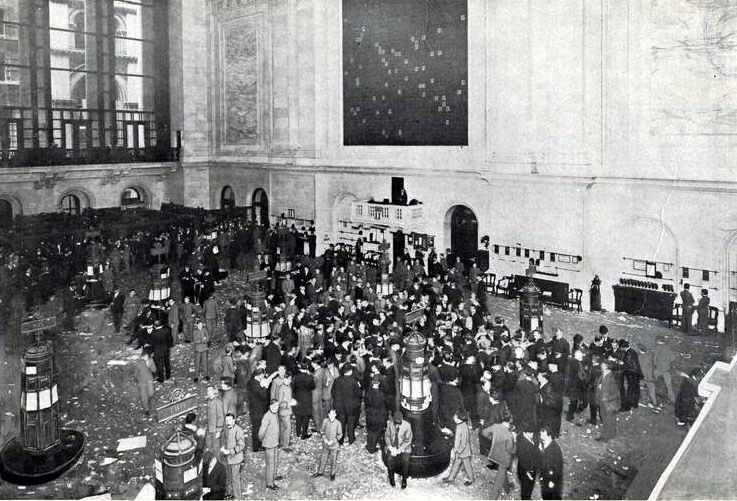
\includegraphics[height=0.34\textheight]{ch8_nyse_floor_1908.jpg}\\[1mm]
\imgcap{New York Stock Exchange, 1908}
\imgcredit{https://commons.wikimedia.org/wiki/File:Stockexchange.jpg}{Photo: Helen D. Van Eaton, Leslie's Monthly Magazine (1908); public domain; Wikimedia Commons}
\end{column}
\begin{column}{0.56\textwidth}
\begin{itemize}
    \item 1982--1986: ARCH and GARCH \refEng, \refBol: volatility as a filtered conditional variance of daily returns
    \item 1992--2004: QML theory \refBW, \refLH, \refLum, \refFZa; components \refEL; DCC \refEngD
    \item 1998--2008: realised variance \refAB, \refABDL, \refBNSa; bipower variation \refBNSb; noise and kernels \refZMA, \refBNHLSa
    \item 2009--2019: HAR \refCor, Realized GARCH \refHHS, GARCH-MIDAS \refEGS, HARQ \refBPQ, DCC-NL \refELW
    \item Today: high-frequency data are cheap; the questions are statistical (noise, jumps, dimension, evaluation)
\end{itemize}
\end{column}
\end{columns}
\end{frame}


%=============================================================================
\section{Quasi-maximum likelihood for GARCH}
%=============================================================================

\begin{frame}{From TSA to this chapter}
\itemsize{\small}
\begin{itemize}
    \item Known (\atschlink{https://danpele.github.io/Time-Series-Analysis/EN/Courses/chapter5_conditional_volatility_garch.pdf}{TSA, Chapter 5}): GARCH(1,1), GJR, EGARCH, the news impact curve, ML with Gaussian and Student-$t$ errors, QLIKE; (\atschlink{https://danpele.github.io/Time-Series-Analysis/EN/Courses/chapter14_multivariate_garch_models.pdf}{TSA, Chapter 14}): CCC and DCC
    \item New here
    \begin{itemize}
        \item why Gaussian ML still works when returns are not Gaussian, and which standard errors are then valid
        \item volatility with a slow, macro-driven component; volatility measured from intraday prices, with its own sampling error
        \item models that use realised measures; evaluation against a noisy target; covariance matrices with many assets
    \end{itemize}
    \item Stochastic volatility (a latent log-variance with its own shock): \atschlink{https://danpele.github.io/Advanced-Time-Series/EN/Courses/chapter6_state_space_models_bayesian_filtering.pdf}{Chapter 6}; Markov-switching GARCH: \atschlink{https://danpele.github.io/Advanced-Time-Series/EN/Courses/chapter7_regime_switching_models.pdf}{Chapter 7}; VaR and ES backtesting: \atschlink{https://danpele.github.io/Advanced-Time-Series/EN/Courses/chapter9_var_es_backtesting.pdf}{Chapter 9}; rough volatility: \atschlink{https://danpele.github.io/Advanced-Time-Series/EN/Courses/chapter10_long_memory_rough_volatility.pdf}{Chapter 10}
\end{itemize}
\end{frame}

\begin{frame}{The Gaussian quasi-likelihood (1/2): the model}
\itemsize{\small}
\begin{itemize}
    \item The return shock is a volatility times a standardised shock; the variance follows a GARCH(1,1) recursion
    \[ \varepsilon_t = \sigma_t(\theta_0)\,\eta_t, \qquad \sigma^2_t(\theta) = \omega + \alpha\varepsilon^2_{t-1} + \beta\sigma^2_{t-1}(\theta) \]
    \item Notation
    \begin{itemize}
        \item $\varepsilon_t$: the demeaned return of day $t$; $\sigma^2_t(\theta)$: its variance conditional on the past $\mathcal F_{t-1}$ (the information up to day $t-1$)
        \item $\eta_t$: i.i.d. standardised shock, $\E\eta_t = 0$, $\E\eta_t^2 = 1$; its law (Normal, Student-$t$, skewed) is unknown
        \item $\theta = (\omega, \alpha, \beta)$, true value $\theta_0$: $\omega > 0$ sets the level, $\alpha \ge 0$ the reaction to yesterday's squared shock, $\beta \ge 0$ the persistence of yesterday's variance
    \end{itemize}
    \item The recursion starts from an arbitrary $\sigma^2_1$; the effect of the start vanishes geometrically when $\beta < 1$
\end{itemize}
\end{frame}

\begin{frame}{The Gaussian quasi-likelihood (2/2): estimator and score}
\itemsize{\small}
\begin{itemize}
    \item QMLE: maximise the Gaussian log-likelihood, used as an estimating equation even if $\eta_t$ is not Gaussian
    \[ \hat\theta = \arg\max_\theta \sum_{t=1}^T \ell_t(\theta), \qquad \ell_t(\theta) = -\frac12\Big(\ln\sigma^2_t(\theta) + \frac{\varepsilon_t^2}{\sigma^2_t(\theta)}\Big) \]
    \begin{itemize}
        \item $\ell_t$: the Gaussian log-density of day $t$ without its constant; $T$: number of days; $\hat\theta$: the estimate
    \end{itemize}
    \item The score, the gradient of $\ell_t$, has conditional mean zero at the true value
    \[ s_t(\theta) = \frac{\partial\ell_t}{\partial\theta} = \frac12\Big(\frac{\varepsilon_t^2}{\sigma_t^2} - 1\Big)\frac{1}{\sigma^2_t}\frac{\partial\sigma^2_t}{\partial\theta} \]
    \begin{itemize}
        \item at $\theta_0$, $\varepsilon_t^2/\sigma_t^2 = \eta_t^2$, hence $\E(s_t | \mathcal F_{t-1}) = 0$ because $\E\eta_t^2 = 1$
        \item only the conditional variance must be right; the shape of the law of $\eta_t$ is never used
    \end{itemize}
    \item The score is a martingale difference (conditional mean zero given the past)
    \begin{itemize}
        \item a CLT for martingales gives asymptotic normality without independence of $\varepsilon_t$
    \end{itemize}
\end{itemize}
\end{frame}

\begin{frame}{Consistency and asymptotic normality (1/2): stationarity and consistency}
\itemsize{\small}
\begin{itemize}
    \item GARCH(1,1) is strictly stationary if and only if the log of the daily variance multiplier has a negative mean
    \[ \E\ln(\alpha_0\eta_t^2 + \beta_0) < 0 \]
    \begin{itemize}
        \item $\alpha_0\eta_t^2 + \beta_0$: the factor by which a shock to the variance is carried from one day to the next; $\alpha_0, \beta_0$: true values
        \item by Jensen's inequality, weaker than $\alpha_0 + \beta_0 < 1$ (finite variance): IGARCH ($\alpha_0 + \beta_0 = 1$) is strictly stationary, and $\E\varepsilon_t^2$ may be infinite
        \item \refLH, \refLum: GARCH(1,1), including IGARCH; \refBHK, \refFZa: GARCH($p,q$) under strict stationarity
    \end{itemize}
    \item Consistency of $\hat\theta$ \refFZa
    \begin{itemize}
        \item conditions: strict stationarity, $\theta_0$ in a compact parameter set, identifiability ($\eta_t^2$ is not a constant)
        \item no moment of $\varepsilon_t$ is needed
    \end{itemize}
    \item Even explosive GARCH ($\E\ln(\alpha_0\eta^2 + \beta_0) > 0$): $(\hat\alpha, \hat\beta)$ remain consistent and asymptotically normal, $\omega$ is not identified \refJR
\end{itemize}
\end{frame}

\begin{frame}{Consistency and asymptotic normality (2/2): the limit law}
\itemsize{\small}
\begin{itemize}
    \item With $\theta_0$ interior to the parameter set and a finite fourth moment of $\eta_t$, the estimator is asymptotically normal
    \[ \sqrt T(\hat\theta - \theta_0) \to N\big(0, (\kappa_\eta - 1)J^{-1}\big), \qquad J = \E\Big[\frac{1}{\sigma^4_t}\frac{\partial\sigma^2_t}{\partial\theta}\frac{\partial\sigma^2_t}{\partial\theta'}\Big] \]
    \begin{itemize}
        \item $\kappa_\eta = \E\eta_t^4$: kurtosis of the shock ($3$ for the Normal distribution); $\kappa_\eta - 1 = \Var(\eta_t^2)$
        \item $J$: a $3 \times 3$ matrix, the mean outer product of the relative sensitivities $\sigma_t^{-2}\partial\sigma^2_t/\partial\theta$; $\to$: convergence in distribution as $T \to \infty$
        \item reading: the sampling variance of $\hat\theta$ grows linearly with the kurtosis of the shocks
    \end{itemize}
    \item Boundary: if $\alpha_0 = 0$, $\theta_0$ is not interior and the limit is the projection of a normal vector on a cone
    \begin{itemize}
        \item this is why \atschlink{https://danpele.github.io/Time-Series-Analysis/EN/Courses/chapter5_conditional_volatility_garch.pdf}{TSA, Chapter 5} tests ARCH effects one-sided
    \end{itemize}
\end{itemize}
\end{frame}

\begin{frame}{The sandwich and the Bollerslev--Wooldridge standard errors (1/2)}
\itemsize{\small}
\begin{itemize}
    \item General QML result: the asymptotic variance is a ``sandwich'' of two matrices
    \[ \sqrt T(\hat\theta - \theta_0) \to N(0, A^{-1}B\,A^{-1}), \qquad A = -\E\frac{\partial^2\ell_t}{\partial\theta\,\partial\theta'}, \qquad B = \E\,s_ts_t' \]
    \begin{itemize}
        \item $A$: the expected negative Hessian (curvature of the log-likelihood); $B$: the variance of the score $s_t$
        \item if the likelihood is the true one, $A = B$ (information equality) and the variance reduces to $A^{-1}$; under QML, $A \ne B$
    \end{itemize}
    \item For GARCH both matrices are proportional to $J$ (\atsapplink{atsapp1}{atssrc1}{Appendix})
    \[ A = \tfrac12J, \qquad B = \tfrac{\kappa_\eta - 1}{4}J, \qquad A^{-1}B\,A^{-1} = (\kappa_\eta - 1)J^{-1} \]
    \begin{itemize}
        \item the sandwich recovers the limit law of the previous slide, for any law of $\eta_t$ with $\kappa_\eta < \infty$
    \end{itemize}
\end{itemize}
\end{frame}

\begin{frame}{The sandwich and the Bollerslev--Wooldridge standard errors (2/2)}
\itemsize{\small}
\begin{itemize}
    \item Three ways to compute standard errors (s.e.)
    \begin{itemize}
        \item Hessian only: $A^{-1} = 2J^{-1}$, correct only if $\kappa_\eta = 3$; too small by the factor $\sqrt{(\kappa_\eta - 1)/2}$ when $\kappa_\eta > 3$
        \item outer product of the scores (OPG): $B^{-1} = \frac{4}{\kappa_\eta - 1}J^{-1}$, even smaller when $\kappa_\eta > 3$
        \item sandwich \refBW: $\hat A^{-1}\hat B\hat A^{-1}$, valid whatever the law of $\eta_t$ (with $\kappa_\eta < \infty$)
    \end{itemize}
    \item Estimates used by Bollerslev and Wooldridge
    \begin{itemize}
        \item $\hat A$: the observed Hessian of $-\frac1T\sum_t\ell_t$ at $\hat\theta$; $\hat B = \frac1T\sum_t\hat s_t\hat s_t'$, with $\hat s_t = s_t(\hat\theta)$ the estimated score
    \end{itemize}
    \item Robust Wald and score tests use the sandwich
    \begin{itemize}
        \item the quasi-likelihood-ratio (quasi-LR) statistic is no longer $\chi^2$, but a weighted sum of $\chi^2_1$ variables (chi-square with one degree of freedom)
    \end{itemize}
\end{itemize}
\end{frame}

\begin{frame}{Hessian against sandwich: a Monte Carlo}
\itemsize{\footnotesize}
\begin{center}
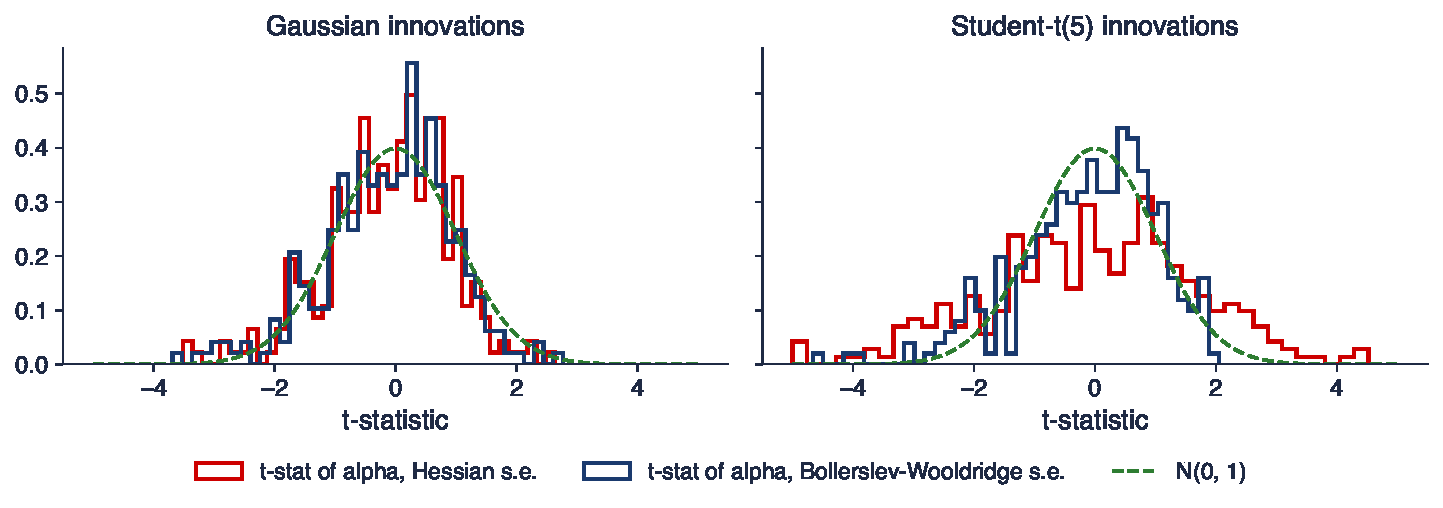
\includegraphics[width=0.97\textwidth,height=0.6\textheight,keepaspectratio]{ats_ch8_qmle_sim.pdf}
\end{center}
\vspace{-0.25cm}
\begin{itemize}
    \item GARCH(1,1) with $(\omega, \alpha, \beta) = (0.05, 0.08, 0.90)$, $T = 2\,000$, 300 replications; Gaussian QML in each; histogram of $(\hat\alpha - \alpha_0)/\widehat{\mathrm{se}}$
\end{itemize}
\quantlet{ATS\_ch8\_qmle}{\qlurl{ATS_ch8_qmle}}
\end{frame}

\begin{frame}{Interpreting the Monte Carlo}
\itemsize{\small}
\begin{itemize}
    \item Gaussian $\eta$: coverage of nominal 95\% intervals for $\alpha$ is 95.0\% (Hessian) and 94.3\% (sandwich): both fine
    \item Student-$t(5)$, $\kappa_\eta = 9$: Hessian intervals cover 73.0\% for $\alpha$ and 74.7\% for $\beta$; sandwich intervals 91.7\% and 92.3\%
    \item The theory predicts the factor $\sqrt{(9 - 1)/2} = 2$ between the two standard errors; the point estimates are the same
    \item With fat tails, a Hessian-based $t$-test of $\alpha$ rejects far too often: report sandwich standard errors by default
\end{itemize}
\end{frame}

\begin{frame}{Robust and naive standard errors in five markets}
\itemsize{\footnotesize}
\begin{center}
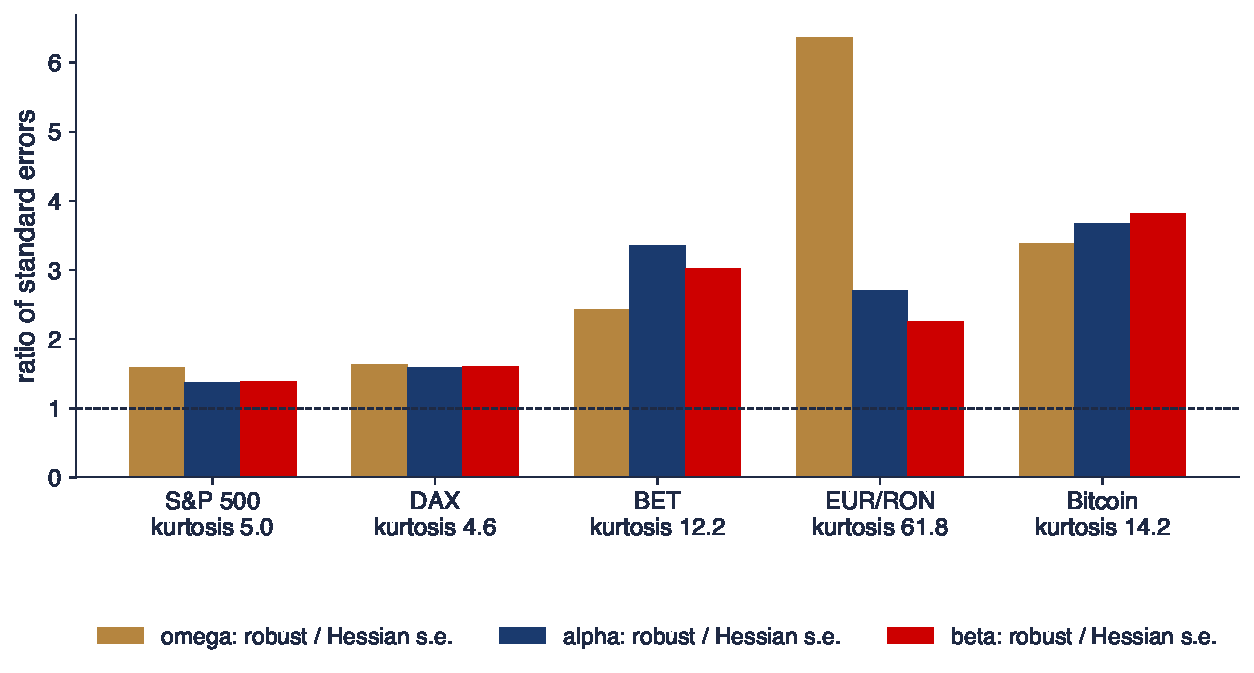
\includegraphics[width=0.97\textwidth,height=0.6\textheight,keepaspectratio]{ats_ch8_qmle_markets.pdf}
\end{center}
\vspace{-0.25cm}
\begin{itemize}
    \item Gaussian QML of GARCH(1,1), daily returns 2010--2026; bars: sandwich s.e. divided by Hessian s.e.; labels: kurtosis $\hat\kappa_\eta$ of the standardised residuals
\end{itemize}
\quantlet{ATS\_ch8\_qmle}{\qlurl{ATS_ch8_qmle}}
\end{frame}

\begin{frame}{Interpreting the five markets}
\itemsize{\small}
\begin{itemize}
    \item S\&P 500: $\hat\alpha = 0.154$ with s.e. 0.013 (Hessian) against 0.018 (sandwich); $\hat\kappa_\eta = 5.0$, theoretical factor 1.42
    \item BET: $\hat\kappa_\eta = 12.2$, the sandwich s.e. of $\hat\alpha$ is 3.36 times larger; EUR/RON (managed float): 2.71 times, $\hat\kappa_\eta = 61.8$
    \item The ratios track $\sqrt{(\hat\kappa_\eta - 1)/2}$ only roughly: in the data $\eta_t$ is not i.i.d., and the sandwich does not need it to be
    \item Student-$t$ ML raises the log-likelihood by 124.4 (S\&P 500) and 233.0 (BET), but is consistent only if the $t$ shape is right; QML needs only the variance equation
\end{itemize}
\end{frame}

\begin{frame}{Recap: QML for GARCH}
\itemsize{\small}
\begin{itemize}
    \item Gaussian QML is consistent if the variance equation is right, whatever the shape of the innovations
    \item Strict stationarity, not finite variance, is what the theory needs; IGARCH and even explosive GARCH are covered
    \item With fat tails, Hessian standard errors are too small by $\sqrt{(\kappa_\eta - 1)/2}$; use Bollerslev--Wooldridge
\end{itemize}
\end{frame}


%=============================================================================
\section{Long-run and short-run volatility}
%=============================================================================

\begin{frame}{GARCH with exogenous variables}
\itemsize{\small}
\begin{itemize}
    \item GARCH-X: yesterday's value of an observed variable enters the variance equation
    \[ \sigma^2_t = \omega + \alpha\varepsilon^2_{t-1} + \beta\sigma^2_{t-1} + \pi'x_{t-1} \]
    \begin{itemize}
        \item $x_{t-1}$: vector of exogenous variables known at the end of day $t-1$; $\pi$: their loadings ($\pi'x$: the weighted sum)
        \item positivity of $\sigma^2_t$: $x_{t-1} \ge 0$ and $\pi \ge 0$, or a specification in logs
    \end{itemize}
    \item Candidates for $x_t$: a realised measure (leads to HEAVY and Realized GARCH below), the VIX, a macro or policy-uncertainty index, trading volume
    \begin{itemize}
        \item QML theory carries over if $x_t$ is stationary and ergodic; its own dynamics need not be modelled for one-step forecasts
        \item multi-step forecasts need a model for $x_t$: this is exactly what Realized GARCH and HEAVY add
    \end{itemize}
    \item A slow variable (a monthly macro series) cannot enter a daily recursion at its own frequency: one needs a component structure (next slides)
\end{itemize}
\end{frame}

\begin{frame}{The component GARCH of Engle and Lee (1/2): the model}
\itemsize{\small}
\begin{itemize}
    \item \refEL: the variance is a slowly moving long-run level $q_t$ plus a transitory deviation from it
    \[ \sigma^2_t = q_t + \alpha(\varepsilon^2_{t-1} - q_{t-1}) + \beta(\sigma^2_{t-1} - q_{t-1}) \]
    \[ q_t = \omega + \rho q_{t-1} + \phi(\varepsilon^2_{t-1} - \sigma^2_{t-1}) \]
    \begin{itemize}
        \item $q_t$: long-run (permanent) component; $\rho$: its persistence, close to 1; $\omega$: its intercept
        \item $\sigma^2_t - q_t$: transitory component; $\alpha$, $\beta$: its reaction and persistence, with $\alpha + \beta < \rho$
        \item $\varepsilon^2_{t-1} - \sigma^2_{t-1}$: the variance surprise of yesterday (mean zero); $\phi$: how much of it moves the long-run level
    \end{itemize}
    \item Both components are driven by the same shock: the model is a restricted GARCH(2,2)
\end{itemize}
\end{frame}

\begin{frame}{The component GARCH of Engle and Lee (2/2): two speeds}
\itemsize{\small}
\begin{itemize}
    \item Half-life: the number of days after which half of a shock to a component has died out
    \[ \mathrm{HL}_q = \frac{\ln(1/2)}{\ln\rho}, \qquad \mathrm{HL}_{\sigma - q} = \frac{\ln(1/2)}{\ln(\alpha + \beta)} \]
    \begin{itemize}
        \item $\mathrm{HL}_q$: half-life of the long-run component; $\mathrm{HL}_{\sigma - q}$: half-life of the transitory component
        \item a persistence $\rho = 0.99$ gives about 69 days; $\alpha + \beta = 0.9$ gives about 6.6 days
        \item GARCH(1,1) forces a single half-life, $\ln 0.5/\ln(\alpha + \beta)$
    \end{itemize}
    \item Two exponentials approximate a slowly decaying (hyperbolic) autocorrelation of squared returns over a finite range of lags
    \begin{itemize}
        \item long memory proper: \atschlink{https://danpele.github.io/Advanced-Time-Series/EN/Courses/chapter10_long_memory_rough_volatility.pdf}{Chapter 10}
    \end{itemize}
\end{itemize}
\end{frame}

\begin{frame}{Component GARCH for the S\&P 500}
\itemsize{\footnotesize}
\begin{center}
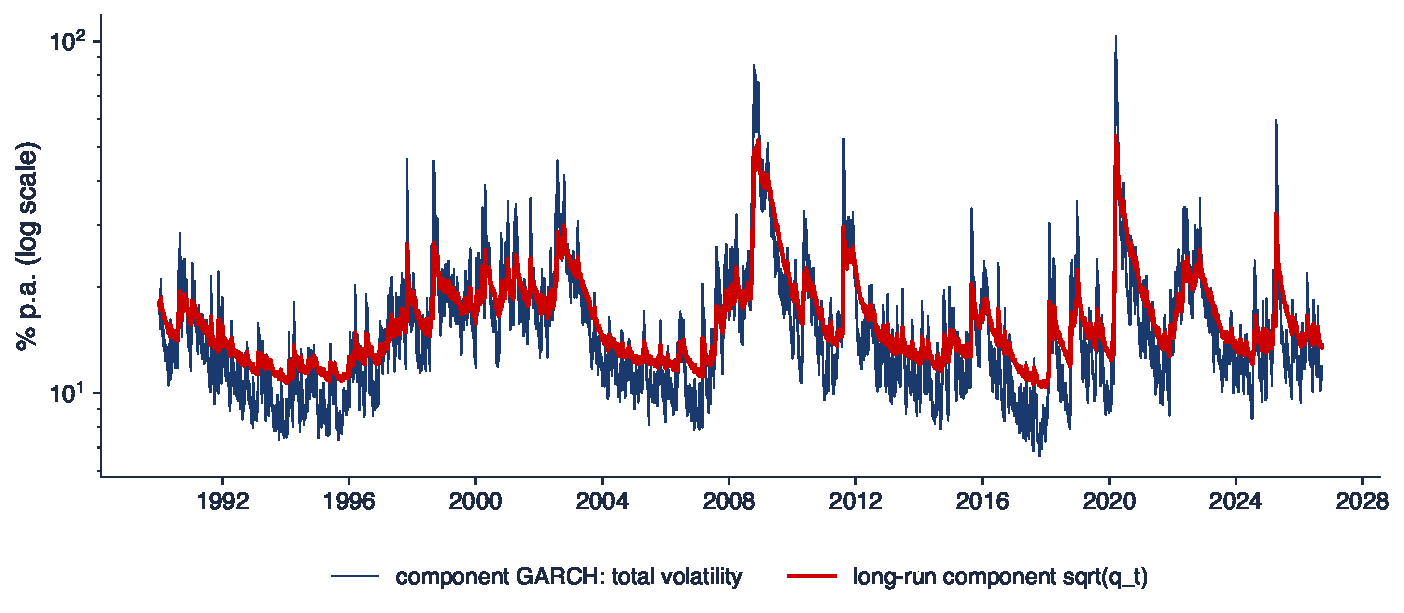
\includegraphics[width=0.97\textwidth,height=0.6\textheight,keepaspectratio]{ats_ch8_cgarch.pdf}
\end{center}
\vspace{-0.25cm}
\begin{itemize}
    \item Daily returns since 1990, $T = 9\,240$; Gaussian QML; annualised total volatility $\sqrt{252\sigma^2_t}$ and long-run component $\sqrt{252q_t}$
\end{itemize}
\quantlet{ATS\_ch8\_components}{\qlurl{ATS_ch8_components}}
\end{frame}

\begin{frame}{Interpreting the component model}
\itemsize{\small}
\begin{itemize}
    \item $\hat\rho = 0.995$, $\hat\phi = 0.026$; transitory part $\hat\alpha + \hat\beta = 0.950$: half-lives 150 days (long run) and 13.6 days (short run)
    \item GARCH(1,1) on the same data: persistence 0.983, one half-life of 41 days, a compromise between the two
    \item Quasi-LR statistic against GARCH(1,1): 44.1; under the null $\phi = 0$ the parameter $\rho$ is not identified (Davies problem), so the $\chi^2_2$ reference is only indicative
    \item After 2008, 2020 and 2025 the long-run level stays high for months while daily volatility has already fallen: this matters for horizons beyond a few weeks
\end{itemize}
\end{frame}

\begin{frame}{GARCH-MIDAS (1/3): a macro-driven long-run component}
\itemsize{\footnotesize}
\begin{columns}[T]
\begin{column}{0.3\textwidth}
\centering

\includegraphics[height=0.26\textheight]{ch8_ghysels_2019.jpg}\\[1mm]
\imgcap{Eric Ghysels, 2019}
\imgcredit{https://commons.wikimedia.org/wiki/File:EricGhysels.jpg}{Photo: Eghysels (2019); CC BY-SA 4.0; Wikimedia Commons}
\end{column}
\begin{column}{0.68\textwidth}
\begin{itemize}
    \item \refEGS: the daily variance is the product of a monthly level $\tau_t$ and a daily factor $g_{i,t}$
    \[ r_{i,t} = \mu + \sqrt{\tau_t\,g_{i,t}}\;\eta_{i,t} \]
    \begin{itemize}
        \item $r_{i,t}$: return of day $i$ of month $t$; $\mu$: mean return; $\eta_{i,t}$: i.i.d. shock with mean 0 and variance 1
    \end{itemize}
    \item Short run: a GARCH(1,1) with mean 1, re-scaled by $\tau_t$
    \[ g_{i,t} = (1 - \alpha - \beta) + \alpha\frac{(r_{i-1,t} - \mu)^2}{\tau_t} + \beta g_{i-1,t} \]
    \begin{itemize}
        \item $\alpha$, $\beta$: reaction and persistence of the daily component, as in GARCH(1,1)
    \end{itemize}
\end{itemize}
\end{column}
\end{columns}
\end{frame}

\begin{frame}{GARCH-MIDAS (2/3): the long-run component}
\itemsize{\small}
\begin{itemize}
    \item Long run: MIDAS (mixed-data sampling) regression of $\ln\tau_t$ on $K$ lags of a monthly variable
    \[ \ln\tau_t = m + \theta\sum_{k=1}^K\varphi_k(w)\,X_{t-k}, \qquad \varphi_k(w) \propto (1 - k/K)^{w - 1} \]
    \begin{itemize}
        \item $X_{t-k}$: the monthly driver $k$ months ago; $m$: intercept; $\theta$: effect of the driver (sign: pro- or countercyclical)
        \item $\varphi_k(w)$: beta lag weights, normalised to sum to 1 and restricted to decay \refGSV; $w \ge 1$: the larger $w$, the faster the decay; $w = 1$: equal weights
    \end{itemize}
    \item Choices of $X$
    \begin{itemize}
        \item realised variance of past months, in levels: $\tau_t = m + \theta\sum_k\varphi_k(w)\mathrm{RV}_{t-k}$, with $\mathrm{RV}_{t-k}$ the sum of squared daily returns of month $t-k$
        \item macro data: industrial production growth, PPI inflation
    \end{itemize}
\end{itemize}
\end{frame}

\begin{frame}{GARCH-MIDAS (3/3): identification, estimation and the variance ratio}
\itemsize{\small}
\begin{itemize}
    \item $\tau_t$ is constant within the month and $\E g_{i,t} = 1$: the split is identified by the different frequencies, without a filter for a latent variable
    \begin{itemize}
        \item Gaussian QML of all parameters $(\mu, \alpha, \beta, m, \theta, w)$ in one step; sandwich standard errors
    \end{itemize}
    \item Variance ratio: the share of the variation of log volatility explained by the long-run component
    \[ \mathrm{VR} = \frac{\Var(\ln\tau_t)}{\Var(\ln(\tau_t\,g_{i,t}))} \in [0, 1] \]
    \begin{itemize}
        \item VR close to 0: the long-run component is almost flat; close to 1: it carries most of the variation
        \item a macro variable can be significant ($\hat\theta \ne 0$) and still explain little of daily volatility (small VR)
    \end{itemize}
    \item Inference on $w$ is nonstandard when $\theta = 0$ ($w$ is then not identified) and at the boundary $w = 1$
    \item Extensions: two-sided weights, several regressors, a second (daily) component \refCK; forecasts beyond one month use only the long-run part
\end{itemize}
\end{frame}

\begin{frame}{Case study: Engle, Ghysels and Sohn (2013) on our data}
\itemsize{\small}
\begin{itemize}
    \item \textbf{Question} of \refEGS: does the stock market's long-run volatility move with macroeconomic fundamentals (output growth, inflation)?
    \begin{itemize}
        \item their sample of US stock returns is much longer than ours; their benchmark long-run component is a fixed-window realised variance
    \end{itemize}
    \item \textbf{Our replication}: S\&P 500 daily returns, common sample from 04.01.1993, $T = 8\,482$; $K = 36$ monthly lags; restricted beta weights
    \begin{itemize}
        \item three long-run drivers: monthly realised variance (sum of squared daily returns), industrial production growth (FRED INDPRO), PPI inflation (FRED WPSFD49207)
        \item all models against GARCH(1,1) on the same days; QML with sandwich standard errors
    \end{itemize}
    \item Extension for a project: Romanian industrial production and the BET (Seminar 8, B5); real-time vintages of the macro data
\end{itemize}
\end{frame}

\begin{frame}{GARCH-MIDAS for the S\&P 500}
\itemsize{\footnotesize}
\begin{center}
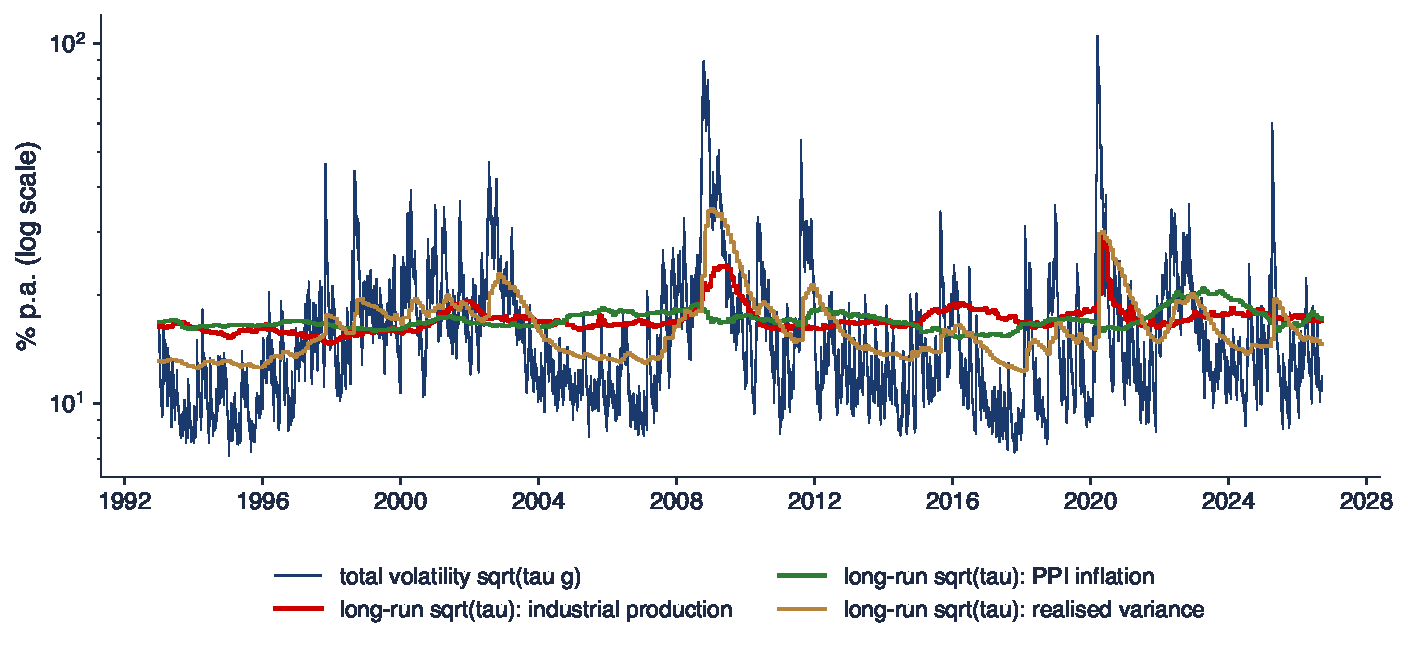
\includegraphics[width=0.97\textwidth,height=0.6\textheight,keepaspectratio]{ats_ch8_garch_midas.pdf}
\end{center}
\vspace{-0.25cm}
\begin{itemize}
    \item Annualised $\sqrt{252\tau_tg_{i,t}}$ of the industrial-production model and the long-run components $\sqrt{252\tau_t}$ of the three models
\end{itemize}
\quantlet{ATS\_ch8\_components}{\qlurl{ATS_ch8_components}}
\end{frame}

\begin{frame}{GARCH-MIDAS estimates}
\itemsize{\small}
\begin{center}
\scriptsize
\begin{tabular}{lcccccc}
\toprule
\textbf{Long-run driver} & $\hat\alpha$ & $\hat\beta$ & $\hat\theta$ (s.e.) & $\hat w$ & VR (\%) & BIC \\
\midrule
realised variance (levels) & 0.119 & 0.841 & 0.0225 (0.0058) & 5.939 & 25.1 & 22710.0 \\
industrial production growth & 0.110 & 0.870 & \ensuremath{-}0.551 (0.353) & 3.692 & 4.5 & 22732.5 \\
PPI inflation & 0.108 & 0.873 & 0.753 (1.260) & 1.000 & 2.2 & 22733.3 \\
GARCH(1,1) & & & & & & 22721.9 \\
\bottomrule
\end{tabular}
\end{center}
\begin{itemize}
    \item Same days for all models; BIC $= -2\ln L + k\ln T$ (lower is better); s.e.: Bollerslev--Wooldridge
\end{itemize}
\end{frame}

\begin{frame}{Interpreting GARCH-MIDAS}
\itemsize{\small}
\begin{itemize}
    \item Realised variance as the slow driver: $\hat\theta = 0.0225$ ($t = 3.86$), VR = 25.1\%, BIC below GARCH(1,1): a long-run component exists
    \item Industrial production: $\hat\theta = \ensuremath{-}0.551$ ($t = \ensuremath{-}1.56$), the countercyclical sign of \refEGS, but VR only 4.5\% and a higher BIC than GARCH(1,1)
    \item PPI inflation: $\hat w$ at the boundary 1 (flat weights) and $\hat\theta$ imprecise: no evidence in 1993--2026
    \item Replication verdict: the qualitative sign survives, the strength does not; macro effects need long samples with deep recessions, which is why the original study uses a much longer history
\end{itemize}
\end{frame}

\begin{frame}{Recap: Long-run components}
\itemsize{\small}
\begin{itemize}
    \item Volatility has at least two speeds; a single GARCH persistence averages them
    \item GARCH-MIDAS lets a monthly variable drive the long-run level; identification comes from the mixed frequencies
    \item Report VR and BIC next to $\hat\theta$: significance is not importance
\end{itemize}
\end{frame}


%=============================================================================
\section{Realised measures: theory, noise and kernels}
%=============================================================================

\begin{frame}{Prices as Itô semimartingales (1/2): the model}
\itemsize{\small}
\begin{itemize}
    \item Within day $t$, the log price moves by a drift, a Brownian part scaled by the spot volatility, and jumps
    \[ dX_s = \mu_s\,ds + \sigma_s\,dW_s + dJ_s, \qquad s \in [0, 1] \]
    \begin{itemize}
        \item $X_s$: log price at intraday time $s$ (the day is rescaled to $[0, 1]$); $\mu_s$: drift; $W_s$: standard Brownian motion
        \item $\sigma_s$: stochastic spot (instantaneous) volatility; $J_s$: a jump process with finitely many jumps per day, $\Delta J_s$: the jump at time $s$
    \end{itemize}
    \item Quadratic variation of the day: the diffusive part plus the squared jumps
    \[ \mathrm{QV}_t = \mathrm{IV}_t + \sum_{s \le 1}(\Delta J_s)^2, \qquad \mathrm{IV}_t = \int_0^1\sigma^2_s\,ds \]
    \begin{itemize}
        \item $\mathrm{IV}_t$: integrated variance, the average of the spot variance over the day
        \item without jumps and with $\sigma$ independent of $W$: $r_t | \mathrm{IV}_t \sim N(\int_0^1\mu_s\,ds, \mathrm{IV}_t)$, so IV is the variance that matters for the daily return $r_t$
    \end{itemize}
\end{itemize}
\end{frame}

\begin{frame}{Prices as Itô semimartingales (2/2): realised variance}
\itemsize{\small}
\begin{itemize}
    \item Realised variance: the sum of the $n$ squared intraday returns of the day
    \[ \mathrm{RV}_t = \sum_{i=1}^n r_{t,i}^2, \qquad r_{t,i} = X_{i/n} - X_{(i-1)/n} \]
    \begin{itemize}
        \item $n$: number of intraday intervals (78 five-minute returns in a 6.5-hour session); $r_{t,i}$: log return over the $i$-th interval
        \item $\mathrm{RV}_t \to \mathrm{QV}_t$ in probability as $n \to \infty$: RV measures the total (diffusive plus jump) variation
    \end{itemize}
    \item The drift does not matter in the limit: it is $O(1/n)$ per interval, while the Brownian part is $O(n^{-1/2})$
    \begin{itemize}
        \item volatility becomes observable \emph{ex post}, without a model \refABDL, \refBNSa
    \end{itemize}
\end{itemize}
\end{frame}

\begin{frame}{The central limit theorem for realised variance (1/2)}
\itemsize{\small}
\begin{itemize}
    \item \refBNSa: without jumps, the error of RV shrinks at rate $\sqrt n$ and is mixed normal
    \[ \sqrt n\,(\mathrm{RV}_t - \mathrm{IV}_t) \to MN(0, 2\,\mathrm{IQ}_t), \qquad \mathrm{IQ}_t = \int_0^1\sigma^4_s\,ds \]
    \begin{itemize}
        \item $\mathrm{IQ}_t$: integrated quarticity, the daily average of $\sigma^4_s$; it sets the size of the error
        \item $MN$ (mixed normal): normal given the path of $\sigma$, with a random variance $2\,\mathrm{IQ}_t$
        \item the convergence is \emph{stable} in law: one may divide by a random, consistently estimated $\sqrt{\mathrm{IQ}_t}$ and keep the limit
    \end{itemize}
    \item Rate $\sqrt n$: with $n = 78$ and volatility constant within the day, the relative error is about $\sqrt{2/78} \approx 16\%$
    \begin{itemize}
        \item the measurement error $\mathrm{RV}_t - \mathrm{IV}_t$ is heteroskedastic (it scales with $\mathrm{IQ}_t$): HARQ, below, is built on this fact
    \end{itemize}
\end{itemize}
\end{frame}

\begin{frame}{The central limit theorem for realised variance (2/2): feasible intervals}
\itemsize{\small}
\begin{itemize}
    \item Feasible version: estimate IQ by the realised quarticity RQ, then studentise
    \[ \widehat{\mathrm{IQ}}_t = \mathrm{RQ}_t = \frac n3\sum_{i=1}^n r_{t,i}^4, \qquad \frac{\mathrm{RV}_t - \mathrm{IV}_t}{\sqrt{\frac23\sum_i r_{t,i}^4}} \to N(0, 1) \]
    \begin{itemize}
        \item the factor $\frac n3$ makes RQ unbiased under constant volatility, because $\E Z^4 = 3$ for $Z \sim N(0, 1)$
        \item 95\% interval for $\mathrm{IV}_t$: $\mathrm{RV}_t \pm 1.96\sqrt{\frac23\sum_i r_{t,i}^4}$; it may contain negative values
    \end{itemize}
    \item Log version (delta method): an interval for $\ln\mathrm{IV}_t$
    \[ \ln\mathrm{RV}_t \pm 1.96\,\frac{\sqrt{\frac23\sum_i r_{t,i}^4}}{\mathrm{RV}_t} \]
    \begin{itemize}
        \item exponentiated, it never contains negative values and has better coverage in finite samples
    \end{itemize}
\end{itemize}
\end{frame}

\begin{frame}{A simulated market with a known truth}
\itemsize{\small}
\begin{itemize}
    \item One-second grid, $n = 23\,400$ seconds a day; the log spot variance is the sum of two Gaussian AR(1) factors
    \[ \ln\sigma^2_s = c + f^{(1)}_s + f^{(2)}_s \]
    \begin{itemize}
        \item $c$: constant fixing the mean; $f^{(1)}$: slow factor (half-life 60 days, stationary s.d. 0.75); $f^{(2)}$: fast factor (half-life 2 days, s.d. 0.45)
        \item mean IV = 1 (\%$^2$ a day), the mean of the S\&P 500 realised kernel in 2000--2022; leverage: correlation $-0.6$ between price shocks and shocks to the fast factor
    \end{itemize}
    \item Jumps: Poisson with 0.08 jumps a day, sizes $N(0, 0.8^2)$ (\%): jumps make about 5.6\% of quadratic variation
    \item Noise: we observe $Y_s = X_s + u_s$, with $u_s$ i.i.d. $N(0, \omega^2)$ and $\omega = 0.004\%$
    \begin{itemize}
        \item $Y_s$: observed log price; $X_s$: efficient log price; $u_s$: microstructure noise with standard deviation $\omega$; at one second, $2n\omega^2 = 0.75$ (next slides)
    \end{itemize}
    \item Each estimator below is compared with the true IV or QV of the same simulated day
\end{itemize}
\end{frame}

\begin{frame}{Coverage of the feasible CLT}
\itemsize{\footnotesize}
\begin{center}
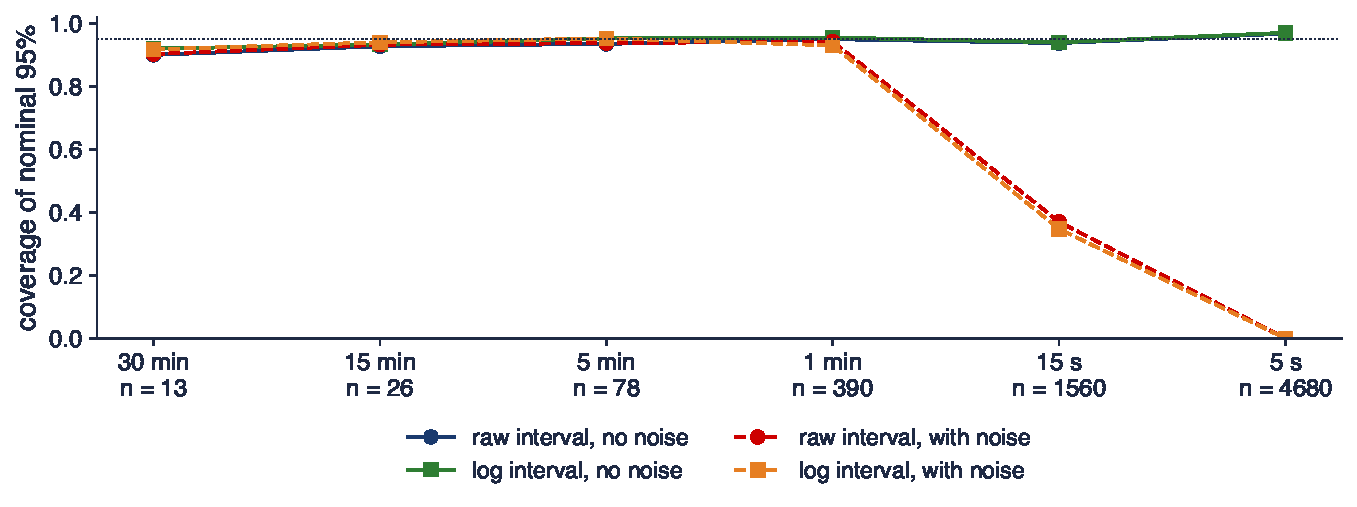
\includegraphics[width=0.97\textwidth,height=0.6\textheight,keepaspectratio]{ats_ch8_rv_clt.pdf}
\end{center}
\vspace{-0.25cm}
\begin{itemize}
    \item 400 simulated days without jumps; 95\% intervals for $\mathrm{IV}_t$ (raw and log) from returns sampled every 30 minutes to every 5 seconds, without and with noise
\end{itemize}
\quantlet{ATS\_ch8\_realised\_measures}{\qlurl{ATS_ch8_realised_measures}}
\end{frame}

\begin{frame}{Interpreting the CLT coverage}
\itemsize{\small}
\begin{itemize}
    \item Without noise, coverage approaches 95\% as $n$ grows: raw interval 90.0\% at $n = 13$ and 95.0\% at $n = 390$; the log interval is closer at small $n$ (92.0\%)
    \item With noise, coverage collapses once sampling is too fine: 37.0\% at 15 seconds and 0.0\% at 5 seconds; at 1 minute it is still 94.2\%
    \item The interval shrinks like $n^{-1/2}$ while the noise bias grows like $n$: the CLT is a statement about the efficient price, not about the observed one
    \item Practical rule: 5-minute returns for liquid assets unless a noise-robust estimator is used
\end{itemize}
\end{frame}

\begin{frame}{Where the realised measures come from}
\itemsize{\footnotesize}
\begin{columns}[T]
\begin{column}{0.36\textwidth}
\centering

\includegraphics[height=0.34\textheight]{ch8_barndorff_nielsen_2007.jpg}\\[1mm]
\imgcap{Ole E. Barndorff-Nielsen, 2007}
\imgcredit{https://commons.wikimedia.org/wiki/File:Ole-Barndorff-Nielsen.jpg}{Photo: Thomas Steiner (2007); CC BY-SA 2.5; Wikimedia Commons}
\end{column}
\begin{column}{0.62\textwidth}
\begin{itemize}
    \item \refOMI, version 0.3: daily RV, BV, realised kernels and open-to-close returns for 31 indices, 2000 to 25 February 2022, built from cleaned tick data
    \item its terms: free use if the library and its version are cited; the archived copy keeps the 2022 file available after the shutdown
    \item Bitcoin and Ether trade 24/7 and Binance publishes all one-minute and one-second prices: we compute RV, BV, RQ, tripower quarticity and a realised kernel for each UTC day, 2018--2026
    \item No free source covers equity intraday data after 2022: a project can rebuild them from a licensed feed
\end{itemize}
\end{column}
\end{columns}
\end{frame}

\begin{frame}{Realised volatility across markets}
\itemsize{\footnotesize}
\begin{center}
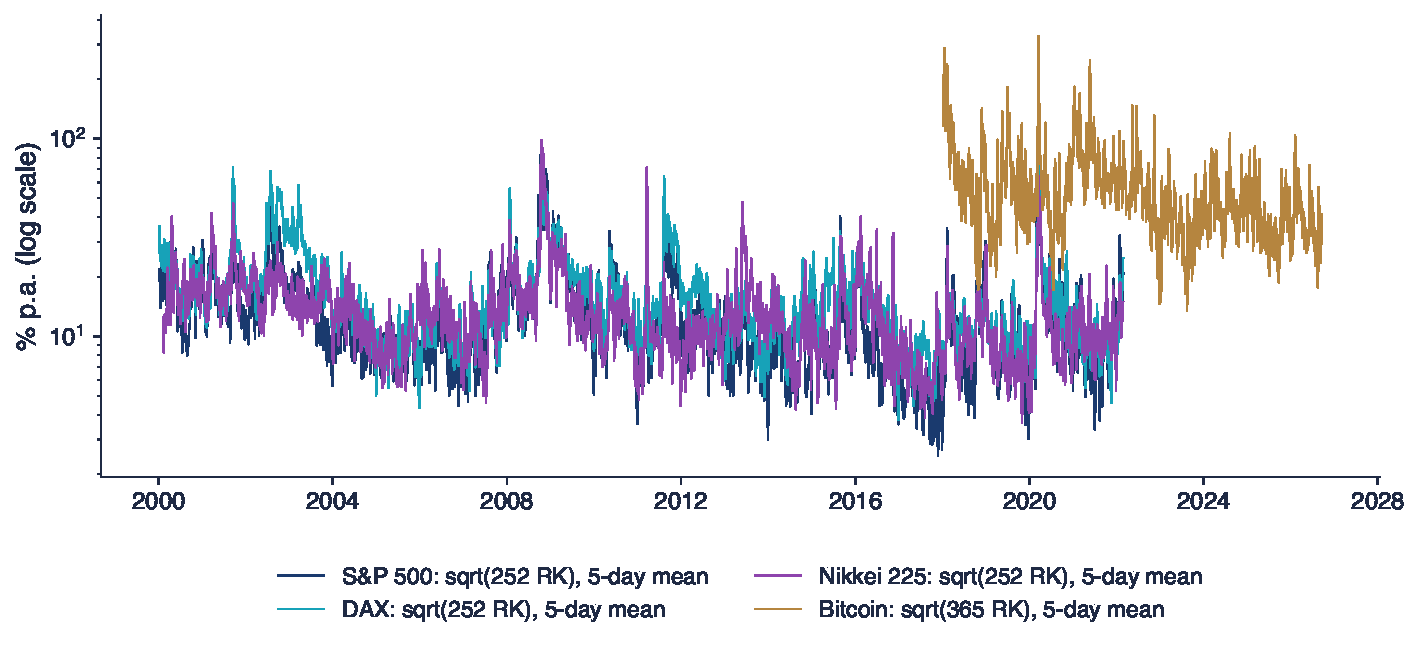
\includegraphics[width=0.97\textwidth,height=0.6\textheight,keepaspectratio]{ats_ch8_rk_overview.pdf}
\end{center}
\vspace{-0.25cm}
\begin{itemize}
    \item Annualised realised kernel, 5-day means: S\&P 500, DAX and Nikkei 225 (Oxford-Man, 2000--2022); Bitcoin (Binance one-minute prices, 2018--2026, 365 days a year)
\end{itemize}
\quantlet{ATS\_ch8\_realised\_measures}{\qlurl{ATS_ch8_realised_measures}}
\end{frame}

\begin{frame}{Interpreting the realised volatilities}
\itemsize{\small}
\begin{itemize}
    \item Average annualised volatility from the kernel: S\&P 500 16.2\%, DAX 19.5\%, Nikkei 16.6\%, Bitcoin 68.4\%
    \item The equity series move together (2002, 2008, 2011, 2020): a common long-run factor, the multivariate theme of the last section
    \item Open-to-close measures miss the overnight return: for daily risk one adds the squared overnight return or scales the measure
    \item Bitcoin has no overnight gap, but its daily volatility is three to four times higher and falls after 2023
\end{itemize}
\end{frame}

\begin{frame}{Microstructure noise (1/2): the bias of RV}
\itemsize{\small}
\begin{itemize}
    \item The observed log price is the efficient price plus a noise term
    \[ Y_{i/n} = X_{i/n} + u_i \]
    \begin{itemize}
        \item $u_i$: i.i.d. noise with variance $\omega^2$, independent of $X$; sources: bid--ask bounce, price discreteness, stale quotes
    \end{itemize}
    \item RV computed from the observed prices at $n$ intervals, $\mathrm{RV}^{(n)}_t$, is biased upwards, and the bias grows with $n$
    \[ \E(\mathrm{RV}^{(n)}_t | X) = \mathrm{IV}_t + 2n\omega^2, \qquad \Var(\mathrm{RV}^{(n)}_t | X) \approx 4n\,\E u^4 \]
    \begin{itemize}
        \item each observed return contains $u_i - u_{i-1}$, with variance $2\omega^2$; summed over $n$ returns this gives $2n\omega^2$
        \item RV diverges as $n \to \infty$: sampling as often as possible is not optimal
        \item derivation of the bias and of the variance: \atsapplink{atsapp2}{atssrc2}{Appendix}  % applink: the noise bias of realised variance
    \end{itemize}
\end{itemize}
\end{frame}

\begin{frame}{Microstructure noise (2/2): diagnostics}
\itemsize{\small}
\begin{itemize}
    \item Two consequences of i.i.d. noise
    \begin{itemize}
        \item $\hat\omega^2 = \mathrm{RV}^{(n)}_t/(2n)$ at the highest frequency estimates the noise variance, since $2n\omega^2$ dominates IV there
        \item returns of the observed price have first-order autocovariance $-\omega^2$: negative autocorrelation is the signature of i.i.d. noise
    \end{itemize}
    \item Signature plot: average $\mathrm{RV}^{(n)}$ against the sampling interval
    \begin{itemize}
        \item a flat region shows the intervals where noise no longer matters
    \end{itemize}
    \item Real noise is not i.i.d.: it is autocorrelated and correlated with the efficient price, especially in quote data \refHLc
\end{itemize}
\end{frame}

\begin{frame}{Optimal sparse sampling}
\itemsize{\small}
\begin{itemize}
    \item Mean square error (MSE) of $\mathrm{RV}^{(n)}$ as an estimator of IV: sampling variance falls, noise bias rises with $n$
    \[ \mathrm{MSE}(n) \approx \underbrace{\frac{2\,\mathrm{IQ}}{n}}_{\text{variance}} + \underbrace{(2n\omega^2)^2}_{\text{bias}^2} + 4n\,\E u^4 + \dots \]
    \item Minimising the first two terms gives the optimal number of intervals \refBR
    \[ n^* \approx \Big(\frac{\mathrm{IQ}}{4\omega^4}\Big)^{1/3} \]
    \begin{itemize}
        \item the optimal grid is coarser when noise ($\omega^2$) is large relative to volatility ($\mathrm{IQ}$)
        \item example (Seminar 8, A3): IV = IQ = 1, $\omega^2 = 1.6\times10^{-5}$ gives $n^* \approx 990$, a return every 24 seconds
    \end{itemize}
    \item The best sparse RV converges only at rate $n^{1/6}$ and discards most data: this motivates estimators that use all observations
    \item Subsampling: average the RV of the $K$ offset grids (starting at second $0, 1, \dots, K-1$); same bias, smaller variance
\end{itemize}
\end{frame}

\begin{frame}{Two scales and realised kernels (1/2)}
\itemsize{\small}
\begin{itemize}
    \item Two-scales RV \refZMA: the fast scale estimates the noise bias of the slow one and removes it
    \[ \mathrm{TSRV} = \overline{\mathrm{RV}}^{(K)} - \frac{\bar n}{n}\,\mathrm{RV}^{(n)}, \qquad \bar n = \frac{n - K + 1}{K} \]
    \begin{itemize}
        \item $\overline{\mathrm{RV}}^{(K)}$: subsampled RV on $K$ offset sparse grids (slow scale), each with about $\bar n$ returns; $\mathrm{RV}^{(n)}$: RV on all $n$ returns (fast scale)
        \item the bias of the slow scale is $2\bar n\omega^2 = \frac{\bar n}{n}\cdot 2n\omega^2$: the correction subtracts it; rate $n^{1/6}$
    \end{itemize}
    \item Pre-averaging \refJLMPV: average returns over blocks before squaring
    \begin{itemize}
        \item rate $n^{1/4}$, the optimal one in the presence of noise; in practice similar to the realised kernel
    \end{itemize}
\end{itemize}
\end{frame}

\begin{frame}{Two scales and realised kernels (2/2): the realised kernel}
\itemsize{\small}
\begin{itemize}
    \item Realised kernel \refBNHLSa: RV plus weighted realised autocovariances
    \[ \mathrm{RK}_t = \gamma_0 + \sum_{h=1}^H k\Big(\frac{h}{H+1}\Big)(\gamma_h + \gamma_{-h}), \qquad \gamma_h = \sum_i r_{t,i}\,r_{t,i-h} \]
    \begin{itemize}
        \item $\gamma_h$: realised autocovariance at lag $h$ ($\gamma_0 = \mathrm{RV}$); $H$: bandwidth, the number of lags used; $k(\cdot)$: weight function with $k(0) = 1$, $k(1) = 0$
        \item Parzen weights: $k(x) = 1 - 6x^2 + 6x^3$ for $x \le \frac12$ and $2(1-x)^3$ for $\frac12 < x \le 1$
        \item the negative $\gamma_1$ created by noise cancels the bias $2n\omega^2$: the same idea as HAC variance estimation (\atschlink{https://danpele.github.io/Advanced-Time-Series/EN/Courses/chapter0_refresher_inference.pdf}{Chapter 0})
    \end{itemize}
    \item Properties
    \begin{itemize}
        \item nonnegative by construction; rate $n^{1/5}$ with $H = c^*\xi^{4/5}n^{3/5}$, where $\xi^2 = \omega^2/\sqrt{\mathrm{IQ}}$ is the noise-to-signal ratio and $c^* = 3.51$ for Parzen \refBNHLSb
        \item it also corrects serially dependent noise of short range, of either sign
    \end{itemize}
\end{itemize}
\end{frame}

\begin{frame}{Estimators against the true quadratic variation}
\itemsize{\footnotesize}
\begin{center}
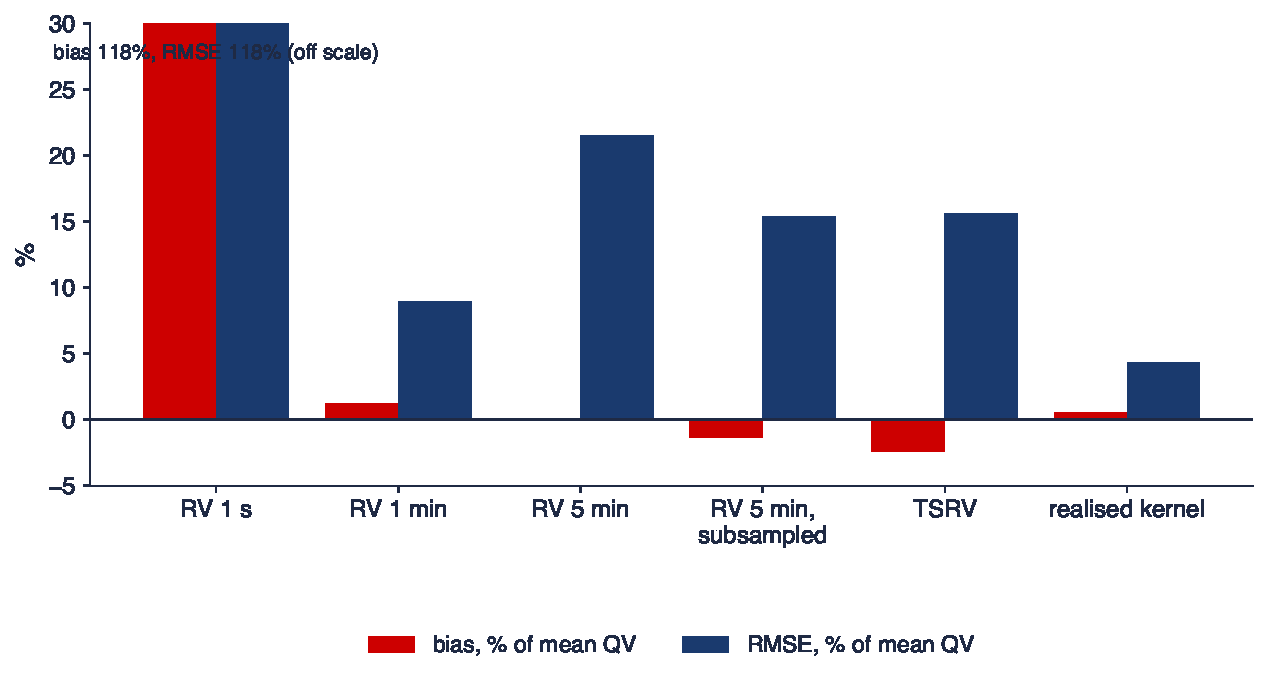
\includegraphics[width=0.97\textwidth,height=0.6\textheight,keepaspectratio]{ats_ch8_kernels.pdf}
\end{center}
\vspace{-0.25cm}
\begin{itemize}
    \item 300 simulated days with jumps and noise; bias and root mean square error relative to the mean QV; TSRV with $K = 300$ seconds; RK with the BNHLS bandwidth (median $H = 31$)
\end{itemize}
\quantlet{ATS\_ch8\_realised\_measures}{\qlurl{ATS_ch8_realised_measures}}
\end{frame}

\begin{frame}{Interpreting the estimator comparison}
\itemsize{\small}
\begin{itemize}
    \item RV at one second is dominated by noise: bias 117.8\% of QV; at one minute the bias is 1.2\% and the RMSE 8.9\%
    \item Five-minute RV is unbiased but noisy (RMSE 21.6\%); subsampling and TSRV reduce it to 15.4\% and 15.6\%
    \item The realised kernel uses all 23\,400 returns: bias 0.5\%, RMSE 4.4\%, the best of the six
    \item All estimators here target QV, jumps included; separating the jump part needs the next section
\end{itemize}
\end{frame}

\begin{frame}{Signature plot and Epps effect: Bitcoin and Ether}
\itemsize{\footnotesize}
\begin{center}
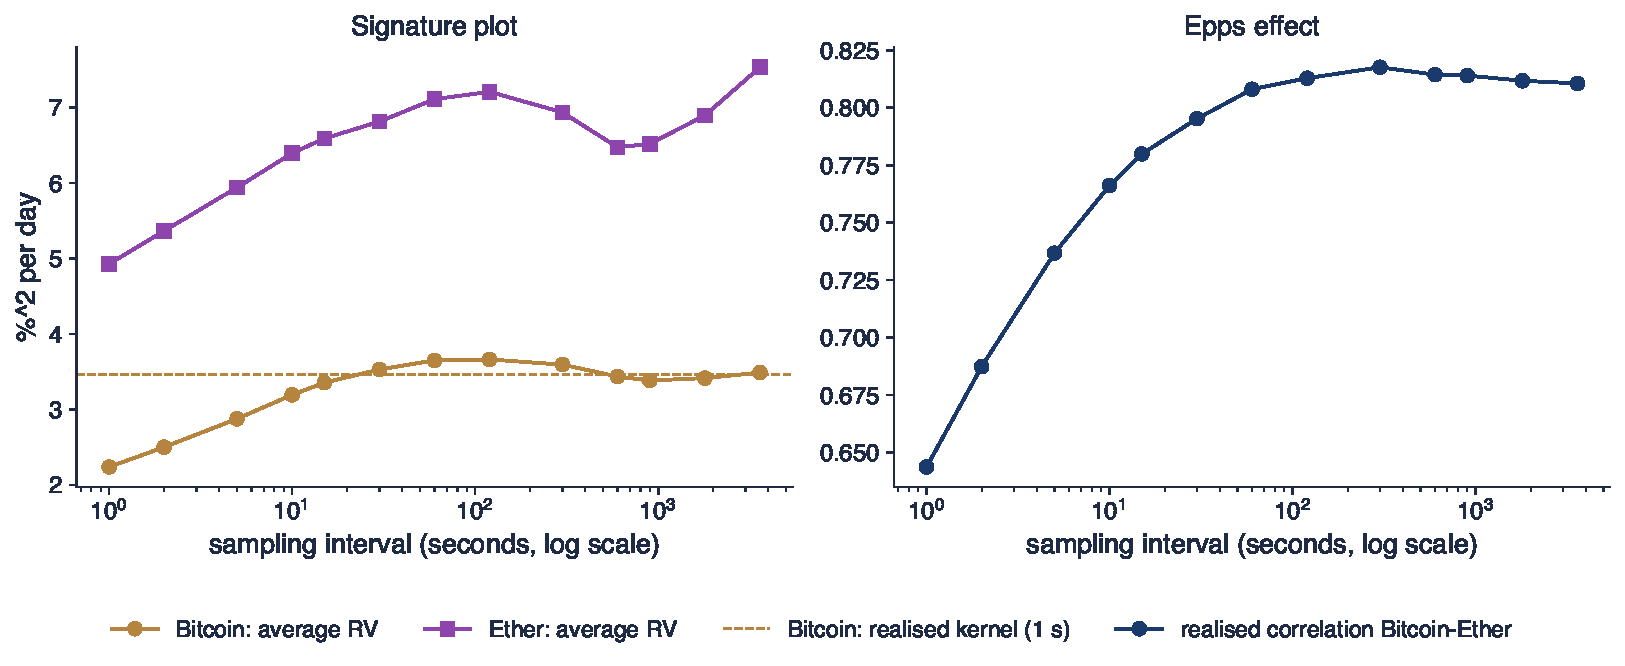
\includegraphics[width=0.97\textwidth,height=0.6\textheight,keepaspectratio]{ats_ch8_signature.pdf}
\end{center}
\vspace{-0.25cm}
\begin{itemize}
    \item Binance one-second prices, August 2026 (31 days); average daily RV by sampling interval (subsampled); realised correlation of the two coins by interval
\end{itemize}
\quantlet{ATS\_ch8\_realised\_measures}{\qlurl{ATS_ch8_realised_measures}}
\end{frame}

\begin{frame}{Interpreting the signature plot}
\itemsize{\small}
\begin{itemize}
    \item Bitcoin: RV is 2.24 at one second, 3.65 at one minute, 3.59 at five minutes: the signature \emph{rises}, the opposite of the i.i.d.-noise prediction
    \item Reason: 52\% of one-second returns are zero (no trade or the same price) and prices adjust gradually, so one-second returns are positively autocorrelated
    \item The realised kernel on one-second data (3.46, median $H = 22$) adds the positive autocovariances back and lands on the flat region of 1--30 minutes
    \item Epps effect \refEpp: realised correlation 0.64 at one second against 0.82 at five minutes; asynchronous trading biases covariances towards zero at high frequency
\end{itemize}
\end{frame}

\begin{frame}{Recap: Realised measures}
\itemsize{\small}
\begin{itemize}
    \item RV estimates QV with error $\sqrt{2\mathrm{IQ}/n}$; the log interval behaves better; stable convergence makes studentization valid
    \item Noise biases RV at high frequency; its sign and size are empirical: look at the signature plot first
    \item Realised kernels use all the data and correct short-range dependent noise; 5-minute RV remains a robust benchmark
\end{itemize}
\end{frame}


%=============================================================================
\section{Jumps: bipower variation and tests}
%=============================================================================

\begin{frame}{Bipower variation (1/2)}
\itemsize{\small}
\begin{itemize}
    \item \refBNSb: sum of products of adjacent absolute returns, rescaled
    \[ \mathrm{BV}_t = \mu_1^{-2}\,\frac{n}{n-1}\sum_{i=2}^n\lvert r_{t,i}\rvert\,\lvert r_{t,i-1}\rvert, \qquad \mu_1 = \E|Z| = \sqrt{2/\pi} \]
    \begin{itemize}
        \item $Z \sim N(0, 1)$; $\mu_1^{-2}$ makes $\mathrm{BV}_t$ consistent for $\mathrm{IV}_t$; $\frac{n}{n-1}$ corrects for the $n-1$ products
        \item $\mathrm{BV}_t \to \mathrm{IV}_t$ even with (finite-activity) jumps: a jump enters only two products, each multiplied by a return of order $n^{-1/2}$
    \end{itemize}
    \item Hence $\mathrm{RV}_t - \mathrm{BV}_t \to \sum_{s \le 1}(\Delta J_s)^2$: a nonparametric estimate of the jump variation of the day
\end{itemize}
\end{frame}

\begin{frame}{Bipower variation (2/2): related estimators}
\itemsize{\small}
\begin{itemize}
    \item Jump-robust quarticity: the tripower quarticity
    \[ \mathrm{TQ}_t = n\,\mu_{4/3}^{-3}\,\frac{n}{n-2}\sum_{i=3}^n\prod_{j=0}^2|r_{t,i-j}|^{4/3}, \qquad \mu_{4/3} = \E|Z|^{4/3} \]
    \begin{itemize}
        \item products of three adjacent absolute returns, each to the power $4/3$; $\mathrm{TQ}_t \to \mathrm{IQ}_t$ even with jumps (RQ does not)
    \end{itemize}
    \item Nearest-neighbour truncation (MedRV, MinRV) \refADS: smaller finite-sample bias from a jump and from zero returns
    \item Threshold (truncated) RV: drop the returns above $c\,n^{-\varpi}$
    \begin{itemize}
        \item $c > 0$: a constant (a multiple of the local volatility); $\varpi \in (0, \frac12)$: the threshold shrinks more slowly than a diffusive return, so only jumps are removed
    \end{itemize}
\end{itemize}
\end{frame}

\begin{frame}{Testing for jumps (1/2): the ratio statistic}
\itemsize{\small}
\begin{itemize}
    \item \refBNSc: without jumps, the difference RV $-$ BV is also mixed normal
    \[ \sqrt n(\mathrm{RV}_t - \mathrm{BV}_t) \to MN(0, \vartheta\,\mathrm{IQ}_t), \qquad \vartheta = \mu_1^{-4} + 2\mu_1^{-2} - 5 = \frac{\pi^2}{4} + \pi - 5 \approx 0.609 \]
    \begin{itemize}
        \item $\vartheta$: a constant that measures how much less efficient BV is than RV
    \end{itemize}
    \item Ratio statistic \refHT: the relative jump contribution, studentised
    \[ z_t = \frac{(\mathrm{RV}_t - \mathrm{BV}_t)/\mathrm{RV}_t}{\sqrt{\frac{\vartheta}{n}\max\big(1, \mathrm{TQ}_t/\mathrm{BV}_t^2\big)}} \to N(0, 1) \]
    \begin{itemize}
        \item one-sided test: reject ``no jump on day $t$'' for large $z_t$
        \item the ratio form and the max adjustment give the best size in their simulations; $\mathrm{TQ}_t/\mathrm{BV}_t^2 \ge 1$ by Jensen when volatility varies within the day
    \end{itemize}
\end{itemize}
\end{frame}

\begin{frame}{Testing for jumps (2/2): in practice}
\itemsize{\small}
\begin{itemize}
    \item A daily test answers ``was there a jump today?''; locating it within the day needs a test on each return standardised by local BV \refLM
    \item Multiple testing: at level $\alpha$ over $T$ days one expects $\alpha T$ false jump days
    \begin{itemize}
        \item use a small $\alpha$ (0.1\%) or a family-wise (FWER) or false-discovery-rate (FDR) correction (\atschlink{https://danpele.github.io/Advanced-Time-Series/EN/Courses/chapter1_forecast_evaluation.pdf}{Chapter 1})
    \end{itemize}
    \item Separating the continuous and jump parts of RV \refABD
    \[ J_t = \mathbb 1(z_t > z_{1-\alpha})\,(\mathrm{RV}_t - \mathrm{BV}_t), \qquad C_t = \mathrm{RV}_t - J_t \]
    \begin{itemize}
        \item $\mathbb 1(\cdot)$: indicator, 1 if the test rejects and 0 otherwise; $z_{1-\alpha}$: the $1-\alpha$ quantile of $N(0, 1)$
        \item $J_t$: jump part, nonzero only on significant days; $C_t$: continuous part
    \end{itemize}
\end{itemize}
\end{frame}

\begin{frame}{Size and power of the ratio test}
\itemsize{\footnotesize}
\begin{center}
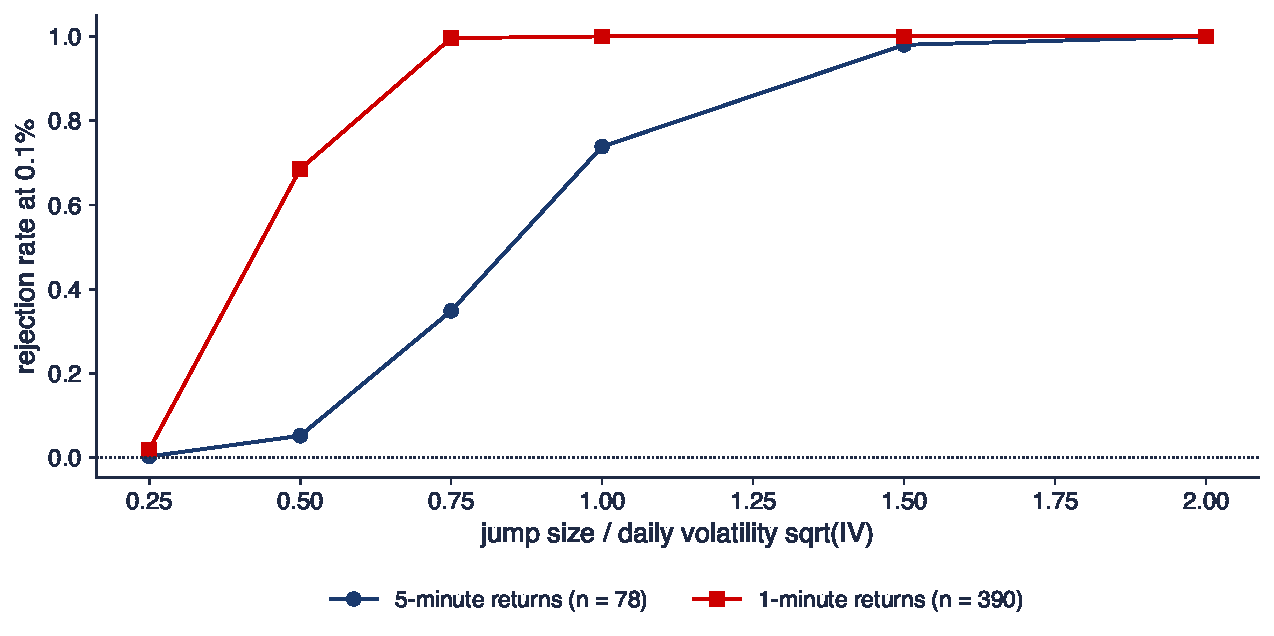
\includegraphics[width=0.97\textwidth,height=0.6\textheight,keepaspectratio]{ats_ch8_jump_power.pdf}
\end{center}
\vspace{-0.25cm}
\begin{itemize}
    \item 2\,000 simulated days (two-factor SV, no jumps), then one jump of size $c\sqrt{\mathrm{IV}_t}$ at a random time; one-sided test at 0.1\% with 5-minute and 1-minute returns
\end{itemize}
\quantlet{ATS\_ch8\_jumps}{\qlurl{ATS_ch8_jumps}}
\end{frame}

\begin{frame}{Interpreting the size and power}
\itemsize{\small}
\begin{itemize}
    \item Size without jumps: 0.0\% (5 minutes) and 0.2\% (1 minute) against the nominal 0.1\%; with i.i.d. noise of the calibrated size still 0.1\% at 1 minute
    \item Power for a jump of half a daily standard deviation: 5\% with 5-minute returns, 68\% with 1-minute returns; for one standard deviation 74\% and 100\%
    \item The power depends on $c\sqrt n$: small jumps are absorbed into the diffusion at coarse sampling (Seminar 8, A6 gives the detection threshold)
    \item The trade-off with noise is the same as for RV: finer sampling raises power until noise and zero returns distort the statistic
\end{itemize}
\end{frame}

\begin{frame}{Jump days of Bitcoin and Ether}
\itemsize{\footnotesize}
\begin{center}
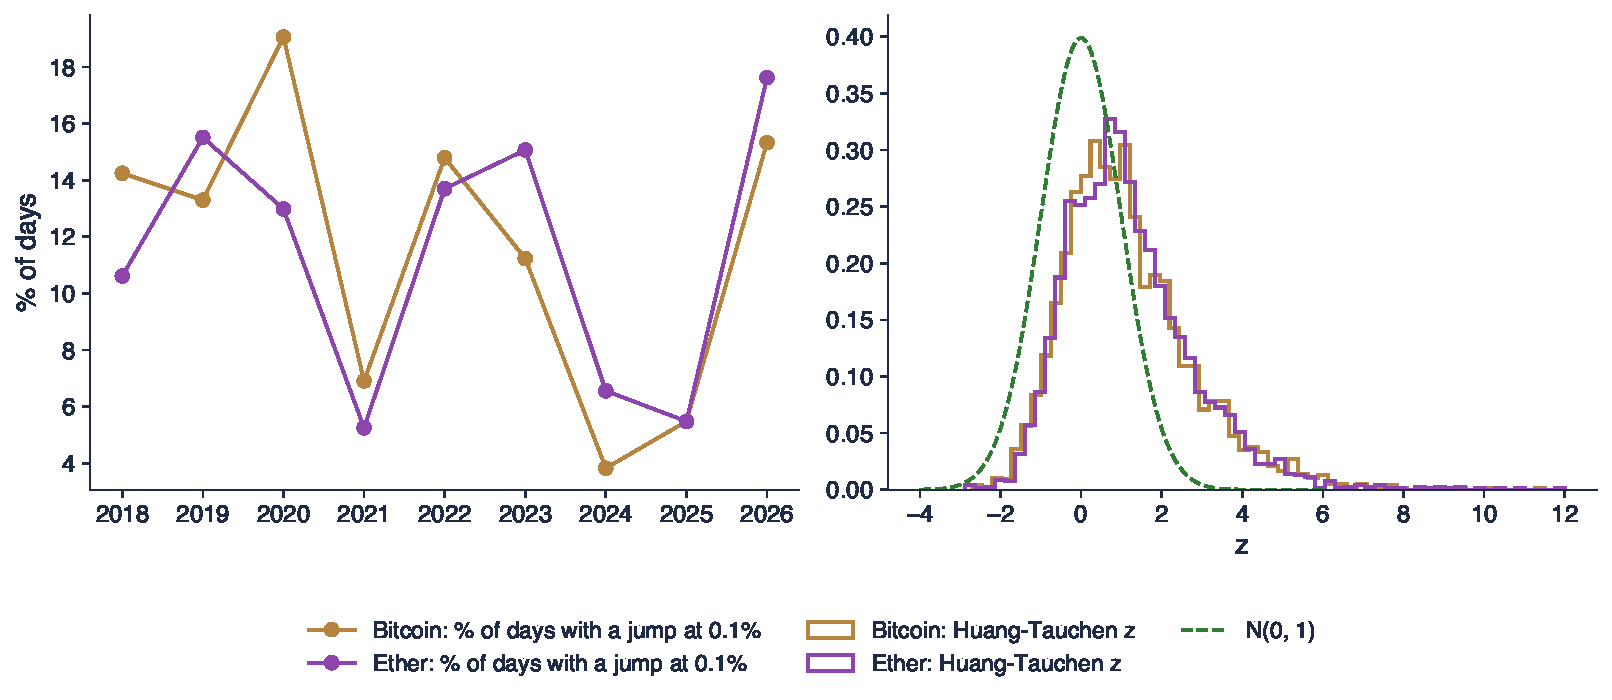
\includegraphics[width=0.97\textwidth,height=0.6\textheight,keepaspectratio]{ats_ch8_jumps_crypto.pdf}
\end{center}
\vspace{-0.25cm}
\begin{itemize}
    \item Huang--Tauchen test with 5-minute returns ($n = 288$ a UTC day), 2018--2026, $T = 3\,165$ days; left: share of jump days at 0.1\% by year; right: distribution of $z_t$ against $N(0, 1)$
\end{itemize}
\quantlet{ATS\_ch8\_jumps}{\qlurl{ATS_ch8_jumps}}
\end{frame}

\begin{frame}{Interpreting the crypto jump tests}
\itemsize{\small}
\begin{itemize}
    \item Bitcoin: 362 jump days (11.4\%) where about 3.2 false rejections are expected; Ether: 355 days (11.2\%)
    \item Yet the jumps are small: they make 3.0\% (Bitcoin) and 2.3\% (Ether) of total variation; the rest is continuous
    \item The whole distribution of $z_t$ is shifted (mean 1.16, not 0): besides jumps, 24-hour intraday seasonality, zero returns and flash moves violate the assumptions of the null
    \item Before calling a day a jump day: standardise returns by an intraday volatility pattern, check zero returns, and control the number of tests
\end{itemize}
\end{frame}

\begin{frame}{Recap: Jumps}
\itemsize{\small}
\begin{itemize}
    \item BV estimates the continuous part; RV $-$ BV the jump part; TQ makes the test robust to jumps in the quarticity
    \item The ratio test has good size in simulations; its power grows with $c\sqrt n$
    \item In real data the null is fragile: many rejections, little jump variation; treat jump counts as model-dependent
\end{itemize}
\end{frame}


%=============================================================================
\section{Forecasting realised variance: HAR and HARQ}
%=============================================================================

\begin{frame}{The HAR model of Corsi (1/2): the regression}
\itemsize{\small}
\begin{itemize}
    \item \refCor: tomorrow's RV is a linear function of the daily, weekly and monthly averages of past RV
    \[ \mathrm{RV}_{t+1} = \beta_0 + \beta_d\mathrm{RV}_t + \beta_w\mathrm{RV}^{(w)}_t + \beta_m\mathrm{RV}^{(m)}_t + u_{t+1} \]
    \[ \mathrm{RV}^{(w)}_t = \frac15\sum_{j=0}^4\mathrm{RV}_{t-j}, \qquad \mathrm{RV}^{(m)}_t = \frac1{22}\sum_{j=0}^{21}\mathrm{RV}_{t-j} \]
    \begin{itemize}
        \item $\mathrm{RV}^{(w)}_t$, $\mathrm{RV}^{(m)}_t$: averages over the last 5 trading days (a week) and the last 22 (a month)
        \item $\beta_d, \beta_w, \beta_m \ge 0$: weights of the three horizons; $\beta_0$: intercept; $u_{t+1}$: forecast error with mean zero
        \item $\beta_d + \beta_w + \beta_m$: the persistence; the closer to 1, the slower volatility returns to its mean
    \end{itemize}
    \item Heterogeneous market hypothesis: daily, weekly and monthly traders react to volatility at their own horizon
    \begin{itemize}
        \item the cascade produces slowly decaying autocorrelations
    \end{itemize}
\end{itemize}
\end{frame}

\begin{frame}{The HAR model of Corsi (2/2): estimation and variants}
\itemsize{\small}
\begin{itemize}
    \item Statistically, HAR is an AR(22) with 19 linear restrictions (step-shaped coefficients)
    \begin{itemize}
        \item short memory, but it mimics long memory over a month
    \end{itemize}
    \item OLS is consistent; the errors are heteroskedastic and, for multi-day targets, overlapping
    \begin{itemize}
        \item use Newey--West \refNW\ (HAC) standard errors
    \end{itemize}
    \item Variants
    \begin{itemize}
        \item log-HAR: the same regression on $\ln\mathrm{RV}$, with near-Gaussian errors; the forecast of RV is $\exp(\hat\mu + \frac12\hat\sigma^2_u)$, with $\hat\mu$ the fitted log value and $\hat\sigma^2_u$ the residual variance
        \item HAR on $\sqrt{\mathrm{RV}}$; $h$-day targets (the average RV over the next $h$ days)
    \end{itemize}
    \item Extensions: continuous and jump parts, HAR-CJ \refABD; positive and negative semivariances \refPS; implied volatility; leverage terms
\end{itemize}
\end{frame}

\begin{frame}{HAR as a restricted AR(22)}
\itemsize{\footnotesize}
\begin{center}
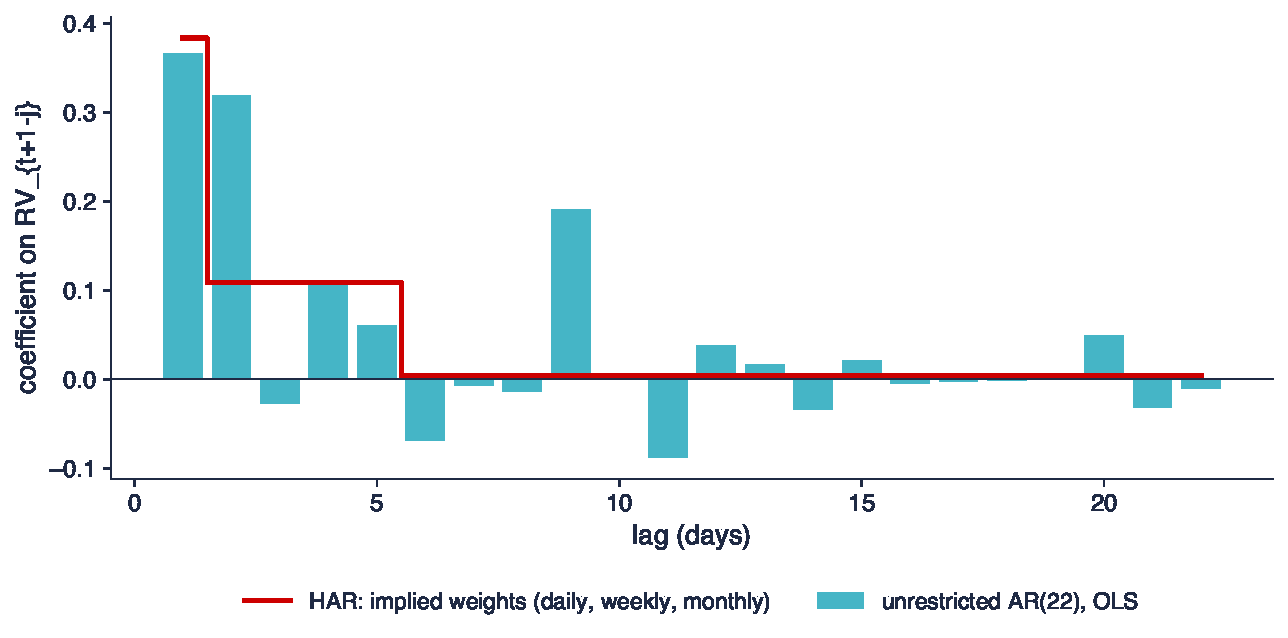
\includegraphics[width=0.97\textwidth,height=0.6\textheight,keepaspectratio]{ats_ch8_har_weights.pdf}
\end{center}
\vspace{-0.25cm}
\begin{itemize}
    \item S\&P 500 (Oxford-Man, 5-minute RV, 2000--2022, $T = 5\,530$): coefficients of an unrestricted AR(22) by OLS and the step weights implied by the HAR estimates
\end{itemize}
\quantlet{ATS\_ch8\_har}{\qlurl{ATS_ch8_har}}
\end{frame}

\begin{frame}{Interpreting the HAR estimates}
\itemsize{\small}
\begin{itemize}
    \item HAR: $\hat\beta_d = 0.275$ (0.104), $\hat\beta_w = 0.522$ (0.140), $\hat\beta_m = 0.094$ (0.078), Newey--West s.e.; $R^2 = 0.560$; persistence $\sum\hat\beta = 0.891$
    \item The AR(22) with 23 coefficients reaches $R^2 = 0.596$ in sample, with erratic coefficients; HAR captures the shape with 4
    \item Log-HAR: $\hat\beta_d = 0.393$, $\hat\beta_w = 0.399$, $\hat\beta_m = 0.153$, $R^2 = 0.719$ on $\ln\mathrm{RV}$; in logs the monthly component matters more
    \item In levels a few crisis days dominate OLS: large standard errors on $\beta_d$ and $\beta_m$; weighted least squares or logs give more stable estimates
\end{itemize}
\end{frame}

\begin{frame}{Forecasting design}
\itemsize{\small}
\begin{itemize}
    \item One day ahead, rolling window of 1\,000 days, re-estimated every day; target $\mathrm{RV}_{t+1}$
    \item Losses: MSE $= (\mathrm{RV} - f)^2$ and QLIKE, both robust to the noise in RV (see below)
    \[ \mathrm{QLIKE} = \frac{\mathrm{RV}}{f} - \ln\frac{\mathrm{RV}}{f} - 1 \ge 0 \]
    \begin{itemize}
        \item $f$: the variance forecast; QLIKE is 0 when $f = \mathrm{RV}$ and penalises under-prediction more than over-prediction
    \end{itemize}
    \item Insanity filter \refBPQ: a forecast outside the range of the in-sample RV is replaced by the in-sample mean
    \begin{itemize}
        \item linear HAR-type forecasts can be negative after a spike; QLIKE is then undefined
        \item the filter is part of the method and must be reported
    \end{itemize}
    \item Diebold--Mariano \refDM\ $t$-statistic of the loss differential against HAR
    \begin{itemize}
        \item Newey--West variance; negative = better than HAR, below $-1.96$ significant at 5\%; several models: the model confidence set \refHLN, \atschlink{https://danpele.github.io/Advanced-Time-Series/EN/Courses/chapter1_forecast_evaluation.pdf}{Chapter 1}
    \end{itemize}
    \item Models: HAR, HAR-CJ (continuous part and jump part, from BV), log-HAR; for Bitcoin and Ether also HARQ
\end{itemize}
\end{frame}

\begin{frame}{HAR extensions out of sample}
\itemsize{\footnotesize}
\begin{center}
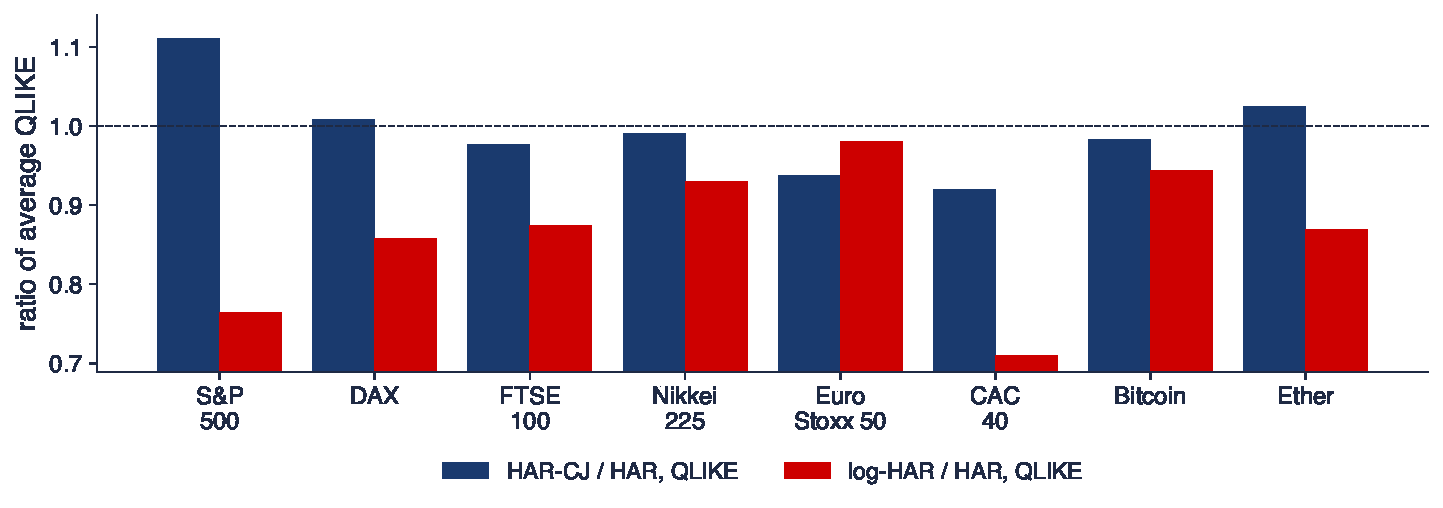
\includegraphics[width=0.97\textwidth,height=0.6\textheight,keepaspectratio]{ats_ch8_har_oos.pdf}
\end{center}
\vspace{-0.25cm}
\begin{itemize}
    \item Average QLIKE relative to HAR (below 1 = better), six Oxford-Man indices (2004--2022) and two cryptocurrencies (from 01.11.2020); 1\,000-day rolling window
\end{itemize}
\quantlet{ATS\_ch8\_har}{\qlurl{ATS_ch8_har}}
\end{frame}

\begin{frame}{Interpreting the out-of-sample HAR comparison}
\itemsize{\small}
\begin{itemize}
    \item Log-HAR beats HAR in QLIKE for 6 of 6 indices: S\&P 500 0.764 (DM \ensuremath{-}2.07), CAC 40 0.709 (DM \ensuremath{-}1.73), FTSE 0.874 (DM \ensuremath{-}5.08)
    \item HAR-CJ helps in 4 of 6 indices, but not for the S\&P 500 (1.110): separating jumps adds estimation noise when jumps are small
    \item The ranking depends on the loss: in MSE the gains of log-HAR are smaller (S\&P 500: 0.837); MSE weighs the crisis days most
    \item Six indices from one data vendor and one period: report all of them, not the best one (data snooping, \atschlink{https://danpele.github.io/Advanced-Time-Series/EN/Courses/chapter1_forecast_evaluation.pdf}{Chapter 1})
\end{itemize}
\end{frame}

\begin{frame}{HARQ (1/2): the measurement error of RV}
\itemsize{\small}
\begin{itemize}
    \item RV is the latent IV plus a measurement error whose variance changes every day
    \[ \mathrm{RV}_t = \mathrm{IV}_t + e_t, \qquad \Var(e_t | \mathrm{IQ}_t) \approx \frac{2\,\mathrm{IQ}_t}{n} \]
    \begin{itemize}
        \item $e_t$: measurement error of day $t$; on volatile days ($\mathrm{IQ}_t$ large) RV is less precise
    \end{itemize}
    \item Errors in variables: in an AR(1) for IV with coefficient $\phi$, the OLS slope on RV is attenuated (\atsapplink{atsapp3}{atssrc3}{Appendix})
    \[ \mathrm{plim}\,\hat\phi = \phi\lambda, \qquad \lambda = \frac{\Var(\mathrm{IV})}{\Var(\mathrm{IV}) + \E\Var(e)} \in (0, 1) \]
    \begin{itemize}
        \item $\lambda$: reliability ratio, the share of the variance of RV that is signal
        \item one constant $\beta_d$ is a compromise: too high on noisy days, too low on precise days
    \end{itemize}
\end{itemize}
\end{frame}

\begin{frame}{HARQ (2/2): a weight that depends on precision}
\itemsize{\small}
\begin{itemize}
    \item \refBPQ: the weight of yesterday's RV moves with its estimated precision
    \[ \mathrm{RV}_{t+1} = \beta_0 + \big(\beta_d + \beta_{dQ}\sqrt{\mathrm{RQ}_t}\big)\mathrm{RV}_t + \beta_w\mathrm{RV}^{(w)}_t + \beta_m\mathrm{RV}^{(m)}_t + u_{t+1} \]
    \begin{itemize}
        \item $\mathrm{RQ}_t$: realised quarticity, the estimate of $\mathrm{IQ}_t$; $\sqrt{\mathrm{RQ}_t}$ is proportional to the standard deviation of $e_t$
        \item $\beta_{dQ} < 0$ expected: the less precise yesterday's RV, the lower its weight
        \item $\sqrt{\mathrm{RQ}_t}$ is demeaned, so $\beta_d$ is the weight on a day of average precision
    \end{itemize}
    \item One extra parameter, still OLS
    \item The original paper: S\&P 500 futures and 27 Dow Jones stocks, gains over HAR in and out of sample
    \begin{itemize}
        \item our replication extends it to Bitcoin and Ether, 2018--2026, where RQ is available from our one-minute data
    \end{itemize}
\end{itemize}
\end{frame}

\begin{frame}{HARQ for Bitcoin: a weight that moves with precision}
\itemsize{\footnotesize}
\begin{center}
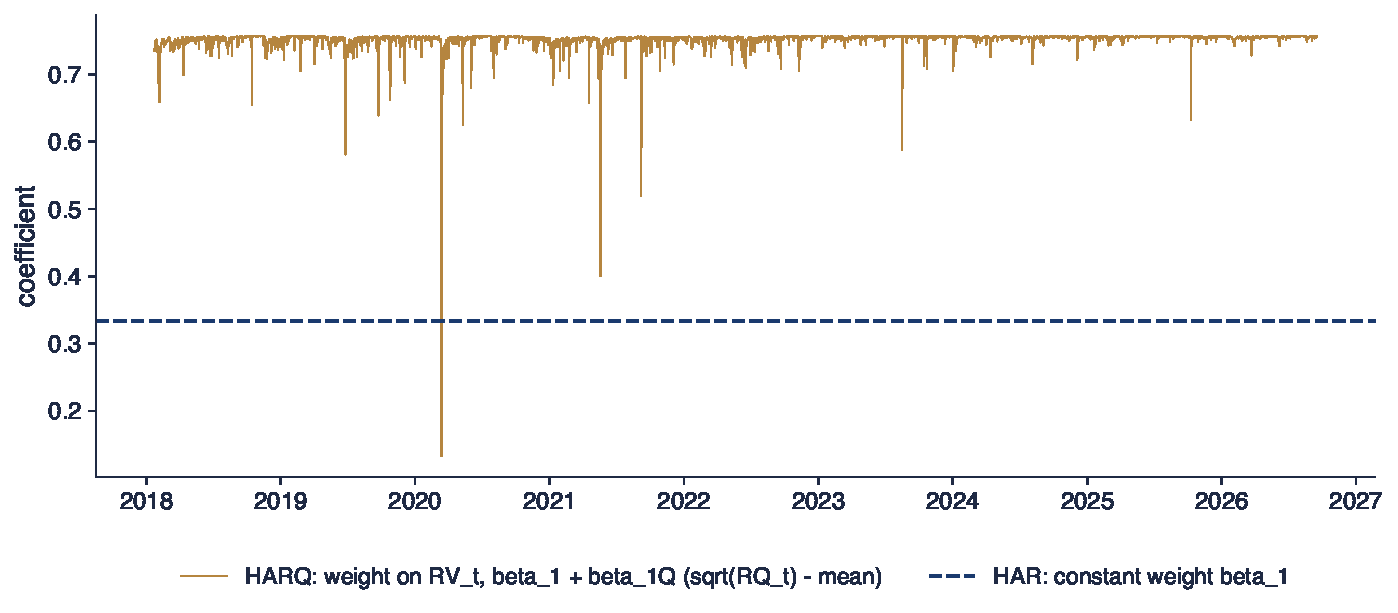
\includegraphics[width=0.97\textwidth,height=0.6\textheight,keepaspectratio]{ats_ch8_harq.pdf}
\end{center}
\vspace{-0.25cm}
\begin{itemize}
    \item Full-sample HARQ on Bitcoin 5-minute RV and RQ: daily weight $\hat\beta_d + \hat\beta_{dQ}(\sqrt{\mathrm{RQ}_t} - \overline{\sqrt{\mathrm{RQ}}})$ against the constant HAR weight
\end{itemize}
\quantlet{ATS\_ch8\_har}{\qlurl{ATS_ch8_har}}
\end{frame}

\begin{frame}{Interpreting HARQ}
\itemsize{\small}
\begin{itemize}
    \item $\hat\beta_{dQ} = \ensuremath{-}0.00021$ ($t = \ensuremath{-}2.7$, Newey--West): negative, as predicted; the daily weight at average precision is 0.752, against 0.334 in HAR
    \item On most days the weight is near 0.76; on the noisiest days it falls (1\% quantile 0.71, minimum 0.13): yesterday's RV is trusted only when it is precise
    \item Out of sample, QLIKE relative to HAR: Bitcoin 0.946 (DM \ensuremath{-}2.44), Ether 0.921 (DM \ensuremath{-}4.50): the gain of the original study carries over to crypto
    \item In MSE the picture differs (Bitcoin 1.163): MSE is dominated by a few extreme days, where HARQ shrinks the most; the AI mini-case checks how fragile the gain is
\end{itemize}
\end{frame}

\begin{frame}{Recap: HAR and HARQ}
\itemsize{\small}
\begin{itemize}
    \item HAR is a parsimonious restricted AR(22) estimated by OLS; logs stabilise it
    \item Out-of-sample gains are loss- and market-specific: report all series, the filter and DM tests
    \item HARQ lets the measurement error of RV set the weight of yesterday: one parameter, a robust gain in QLIKE
\end{itemize}
\end{frame}


%=============================================================================
\section{Realized GARCH and HEAVY}
%=============================================================================

\begin{frame}{Realized GARCH (1/2): the three equations}
\itemsize{\footnotesize}
\begin{itemize}
    \item \refHHS, log-linear form: a return equation, a GARCH equation driven by the realised measure, and a measurement equation
    \[ r_t = \sqrt{h_t}\,z_t, \qquad \ln h_t = \omega + \beta\ln h_{t-1} + \gamma\ln x_{t-1} \]
    \[ \ln x_t = \xi + \varphi\ln h_t + \tau(z_t) + u_t \]
    \begin{itemize}
        \item $h_t$: conditional variance of the return $r_t$; $z_t$: i.i.d. standardised shock; $x_t$: realised measure of day $t$ (here the realised kernel RK)
        \item $\beta$: persistence of $\ln h_t$; $\gamma$: weight of yesterday's realised measure (the news variable that replaces $\varepsilon^2_{t-1}$)
        \item $u_t$: measurement error, i.i.d. $N(0, \sigma^2_u)$, independent of $z_t$
    \end{itemize}
    \item Measurement equation: $x_t$ is a noisy, possibly biased signal of $h_t$
    \begin{itemize}
        \item $\varphi = 1$: $x_t$ proportional to $h_t$; $\xi$ absorbs the scale (open-to-close measure against close-to-close variance)
        \item leverage function $\tau(z) = \tau_1z + \tau_2(z^2 - 1)$: with $\tau_1 < 0$, negative returns raise the next realised measure (news impact, \atschlink{https://danpele.github.io/Time-Series-Analysis/EN/Courses/chapter5_conditional_volatility_garch.pdf}{TSA, Chapter 5})
    \end{itemize}
\end{itemize}
\end{frame}

\begin{frame}{Realized GARCH (2/2): reduced form and estimation}
\itemsize{\small}
\begin{itemize}
    \item Substituting the measurement equation into the GARCH equation: $\ln h_t$ is an AR(1)
    \[ \ln h_t = (\omega + \gamma\xi) + \pi\ln h_{t-1} + \gamma\big(\tau(z_{t-1}) + u_{t-1}\big), \qquad \pi = \beta + \varphi\gamma \]
    \begin{itemize}
        \item $\pi$: persistence of the log variance; multi-step forecasts follow, because $x_t$ has its own equation
    \end{itemize}
    \item Joint QML: the log-likelihood sums a return part and a measurement part
    \[ \ell = -\frac12\sum_t\Big[\underbrace{\ln h_t + z_t^2}_{r_t} + \underbrace{\ln\sigma^2_u + u_t^2/\sigma^2_u}_{x_t}\Big] \]
    \begin{itemize}
        \item comparison with GARCH only through the partial likelihood of $r_t$ (the first part), since GARCH does not model $x_t$
    \end{itemize}
\end{itemize}
\end{frame}

\begin{frame}{HEAVY and the family of realised-measure models}
\itemsize{\footnotesize}
\begin{itemize}
    \item HEAVY \refSS: two GARCH-type equations, one for the return variance and one for the mean of the realised measure
    \[ h_t = \Var(r_t | \mathcal F_{t-1}) = \omega + \alpha\mathrm{RM}_{t-1} + \beta h_{t-1} \]
    \[ \mu_t = \E(\mathrm{RM}_t | \mathcal F_{t-1}) = \omega_R + \alpha_R\mathrm{RM}_{t-1} + \beta_R\mu_{t-1} \]
    \begin{itemize}
        \item $\mathrm{RM}_t$: realised measure of day $t$; $(\omega, \alpha, \beta)$ and $(\omega_R, \alpha_R, \beta_R)$: the parameters of the two equations
        \item each equation is estimated separately by QML; momentum: after a shock, $h_t$ keeps rising while $\mu_t$ catches up
        \item when the realised measure is in the variance equation, the squared return usually adds nothing ($\varepsilon^2_{t-1}$ gets a zero coefficient)
    \end{itemize}
    \item Realized EGARCH \refHH: several realised measures and a richer leverage; score-driven versions exist for fat tails
    \item Compared with HAR: returns and realised measures are modelled jointly, so densities and VaR/ES forecasts are available (\atschlink{https://danpele.github.io/Advanced-Time-Series/EN/Courses/chapter9_var_es_backtesting.pdf}{Chapter 9})
\end{itemize}
\end{frame}

\begin{frame}{Case study: Realized GARCH for the S\&P 500}
\itemsize{\footnotesize}
\begin{center}
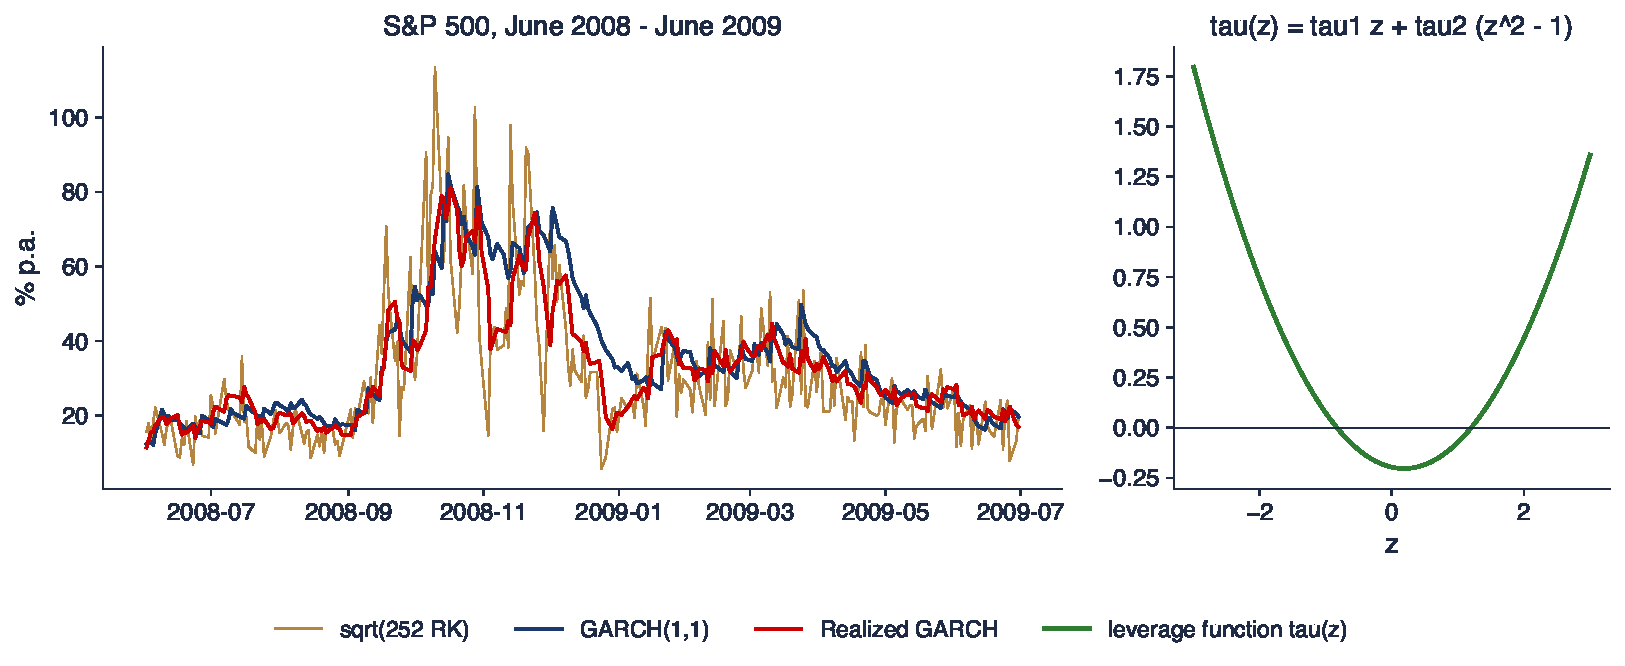
\includegraphics[width=0.97\textwidth,height=0.6\textheight,keepaspectratio]{ats_ch8_rgarch.pdf}
\end{center}
\vspace{-0.25cm}
\begin{itemize}
    \item Open-to-close returns and the Parzen realised kernel (Oxford-Man), 2000--2022, $T = 5\,552$, as in \refHHS; left: the 2008 crisis; right: the estimated leverage function
\end{itemize}
\quantlet{ATS\_ch8\_realized\_garch}{\qlurl{ATS_ch8_realized_garch}}
\end{frame}

\begin{frame}{Realized GARCH estimates}
\itemsize{\small}
\begin{center}
\footnotesize
\begin{tabular}{cccccccc}
\toprule
$\omega$ & $\beta$ & $\gamma$ & $\xi$ & $\varphi$ & $\tau_1$ & $\tau_2$ & $\sigma_u$ \\
\midrule
0.119 & 0.678 & 0.287 & \ensuremath{-}0.456 & 1.012 & \ensuremath{-}0.073 & 0.197 & 0.671 \\
(0.010) & (0.018) & (0.016) & (0.021) & (0.026) & (0.008) & (0.010) & (0.008) \\
\bottomrule
\end{tabular}
\end{center}
\begin{itemize}
    \item Bollerslev--Wooldridge s.e. in brackets; persistence $\hat\pi = \hat\beta + \hat\varphi\hat\gamma = 0.968$ (GARCH(1,1) on the same returns: 0.989)
    \item Partial log-likelihood of the returns: Realized GARCH \ensuremath{-}6899.7, HEAVY \ensuremath{-}6902.8, GJR \ensuremath{-}6998.8, GARCH(1,1) \ensuremath{-}7099.0
    \item HEAVY variance equation: $\hat\alpha = 0.377$ on $\mathrm{RK}_{t-1}$, $\hat\beta = 0.691$
\end{itemize}
\end{frame}

\begin{frame}{Interpreting Realized GARCH}
\itemsize{\small}
\begin{itemize}
    \item $\hat\varphi = 1.012$: the kernel is proportional to the conditional variance; $\hat\xi = \ensuremath{-}0.456$ with $\hat\sigma_u = 0.671$: on average the kernel lies below the conditional variance of the open-to-close return
    \item $\hat\gamma = 0.287$ is large and $\hat\beta = 0.678$ smaller than in GARCH: the realised measure brings information faster than squared returns (left panel, autumn 2008)
    \item Leverage: $\hat\tau_1 = \ensuremath{-}0.073$, $\hat\tau_2 = 0.197$: an asymmetric parabola, larger for negative $z$
    \item The gain in the partial likelihood over GARCH(1,1) (199.3 points) has the direction of the original paper; HEAVY is almost as good with three parameters
\end{itemize}
\end{frame}

\begin{frame}{Recap: Realised-measure GARCH}
\itemsize{\small}
\begin{itemize}
    \item A realised measure in the variance equation beats squared returns as the news variable
    \item Realized GARCH adds a measurement equation: multi-step forecasts, leverage and a joint likelihood
    \item Compare with GARCH only on the partial likelihood of returns
\end{itemize}
\end{frame}


%=============================================================================
\section{Evaluating volatility forecasts with a noisy target}
%=============================================================================

\begin{frame}{The proxy problem and robust losses (1/2)}
\itemsize{\small}
\begin{itemize}
    \item We never see $\sigma^2_t$: a forecast $h_t$ is compared with a proxy $\hat\sigma^2_t$ (squared return, RV, RK)
    \begin{itemize}
        \item the proxy is conditionally unbiased, $\E(\hat\sigma^2_t | \mathcal F_{t-1}) = \sigma^2_t$, but noisy
    \end{itemize}
    \item A loss $L$ is \emph{robust} \refPat\ if the ranking of forecasts by $\E L(\hat\sigma^2_t, h_t)$ equals the ranking by $\E L(\sigma^2_t, h_t)$, for every unbiased proxy \refHLb
    \item Necessary and sufficient condition: a Bregman form (\atschlink{https://danpele.github.io/Advanced-Time-Series/EN/Courses/chapter1_forecast_evaluation.pdf}{Chapter 1}, consistent scoring functions for the mean)
    \[ L(\hat\sigma^2, h) = \tilde C(h) + B(\hat\sigma^2) + C(h)(\hat\sigma^2 - h), \qquad C'(h) < 0 \]
    \begin{itemize}
        \item $C$: a decreasing function of the forecast; $\tilde C$: its antiderivative, $\tilde C' = C$; $B$: any function of the proxy alone (it does not affect the ranking)
    \end{itemize}
\end{itemize}
\end{frame}

\begin{frame}{The proxy problem and robust losses (2/2)}
\itemsize{\small}
\begin{itemize}
    \item Robust: MSE and QLIKE, the members of degree 2 and degree 0 of the homogeneous robust family
    \[ \mathrm{MSE} = (\hat\sigma^2 - h)^2, \qquad \mathrm{QLIKE} = \frac{\hat\sigma^2}{h} - \ln\frac{\hat\sigma^2}{h} - 1 \]
    \begin{itemize}
        \item degree: how the loss scales when proxy and forecast are multiplied by the same constant; QLIKE (degree 0) is scale-free and penalises under-prediction more
    \end{itemize}
    \item Not robust: MAE $= |\hat\sigma^2 - h|$, MSE on logs $(\ln\hat\sigma^2 - \ln h)^2$, MSE on standard deviations
    \begin{itemize}
        \item with a noisy proxy they reward forecasts that are biased downwards
    \end{itemize}
    \item Example: with $\hat\sigma^2 = r^2$, the MSE-log optimum is $h^* = \exp(\E\ln r^2) = 0.28\,\sigma^2$
    \begin{itemize}
        \item because $r^2 = \sigma^2\chi^2_1$ for a Gaussian return and $\E\ln\chi^2_1 = -1.27$: MSE-log prefers a forecast far below the truth
    \end{itemize}
\end{itemize}
\end{frame}

\begin{frame}{Robust and non-robust losses}
\itemsize{\footnotesize}
\begin{center}
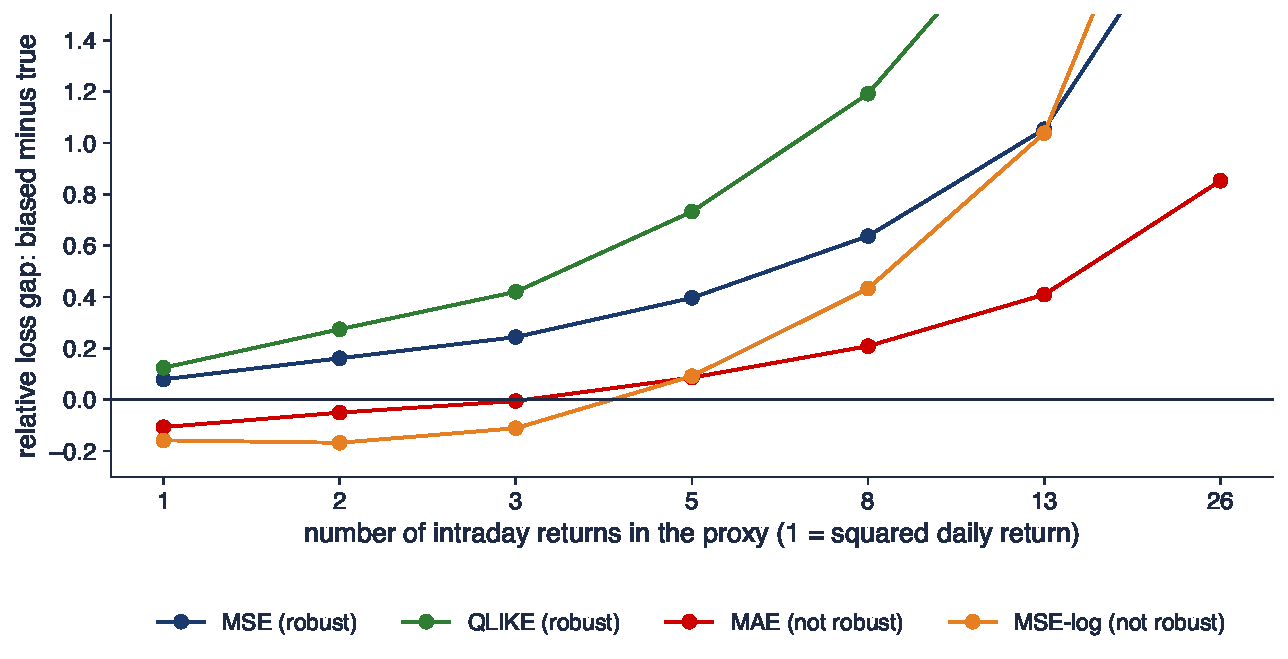
\includegraphics[width=0.97\textwidth,height=0.6\textheight,keepaspectratio]{ats_ch8_patton.pdf}
\end{center}
\vspace{-0.25cm}
\begin{itemize}
    \item True variance against a forecast biased down by the factor 0.6; proxy = RV from $n$ intraday returns ($n = 1$: squared daily return); relative gap of expected losses, above zero = the true variance wins
\end{itemize}
\quantlet{ATS\_ch8\_robust\_loss}{\qlurl{ATS_ch8_robust_loss}}
\end{frame}

\begin{frame}{Interpreting the robustness experiment}
\itemsize{\small}
\begin{itemize}
    \item With the squared return as proxy, MAE prefers the biased forecast (gap \ensuremath{-}10.7\%) and so does MSE-log (\ensuremath{-}15.8\%); MSE (7.9\%) and QLIKE (12.5\%) do not
    \item With $n = 5$ intraday returns all four losses rank correctly: a precise proxy makes non-robust losses ``almost robust 
efHLb
    \item The danger is largest exactly where realised measures are unavailable: daily data, emerging markets, long histories
    \item Rule: evaluate volatility forecasts with QLIKE (and MSE), against the best available proxy
\end{itemize}
\end{frame}

\begin{frame}{Seven forecasts of S\&P 500 volatility}
\itemsize{\footnotesize}
\begin{center}
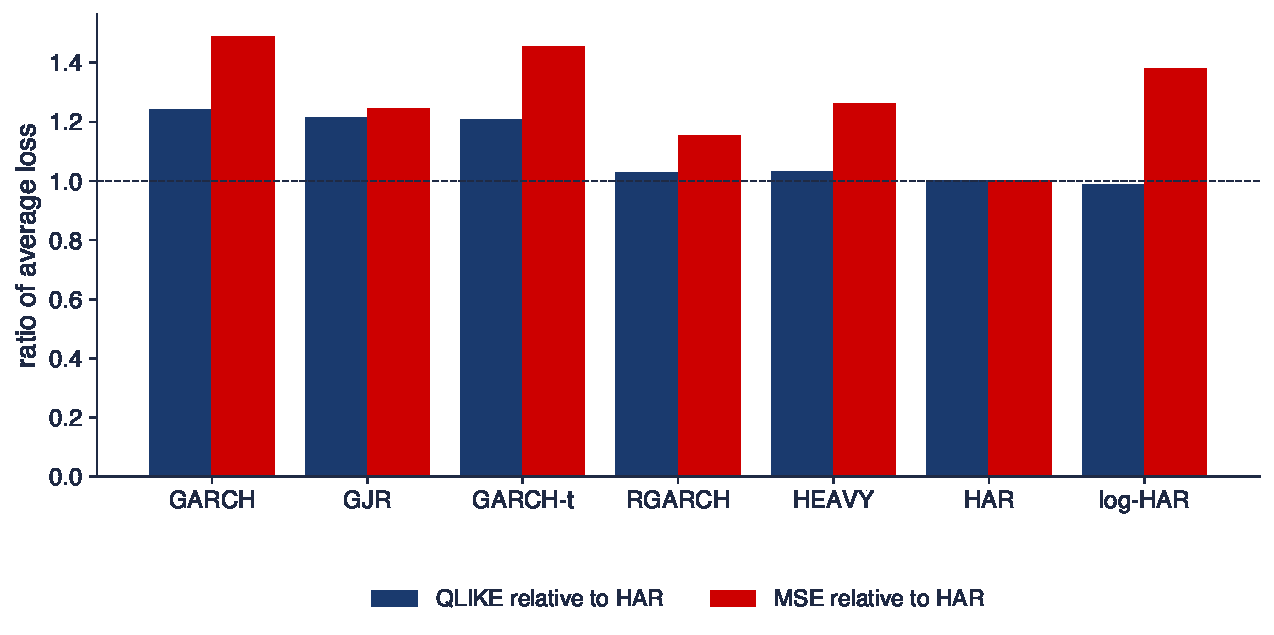
\includegraphics[width=0.97\textwidth,height=0.6\textheight,keepaspectratio]{ats_ch8_vol_oos.pdf}
\end{center}
\vspace{-0.25cm}
\begin{itemize}
    \item Open-to-close variance, one day ahead, 2016--2022 ($1\,537$ days); expanding window from 2000, parameters re-estimated every 250 days; proxy: realised kernel
\end{itemize}
\quantlet{ATS\_ch8\_robust\_loss}{\qlurl{ATS_ch8_robust_loss}}
\end{frame}

\begin{frame}{Interpreting the forecast comparison}
\itemsize{\small}
\begin{itemize}
    \item QLIKE: HAR 0.328, log-HAR 0.324, Realized GARCH 0.337, HEAVY 0.339, GARCH-$t$ 0.396, GJR 0.398, GARCH 0.407
    \item DM against HAR (QLIKE): GARCH 8.62, GJR 6.27, Realized GARCH 1.42, log-HAR \ensuremath{-}0.37: realised-measure models beat return-only models clearly; among them the differences are small
    \item In MSE, HAR (1.60) leads and the DM statistics are smaller: the 2020 crash dominates the squared errors
    \item One proxy (RK) for all models: the HAR family is fitted to that same measure, which favours it; a fair comparison also tries another proxy (RV, BV)
\end{itemize}
\end{frame}

\begin{frame}{Recap: Evaluation}
\itemsize{\small}
\begin{itemize}
    \item Only losses of the Patton class keep the ranking under a noisy unbiased proxy: MSE and QLIKE
    \item Realised-measure models beat return-only GARCH one day ahead; DM and the MCS of \atschlink{https://danpele.github.io/Advanced-Time-Series/EN/Courses/chapter1_forecast_evaluation.pdf}{Chapter 1} quantify by how much
    \item State the proxy, the loss, the window and the filter: each can change the ranking
\end{itemize}
\end{frame}


%=============================================================================
\section{Multivariate GARCH and large covariance matrices}
%=============================================================================

\begin{frame}{From one variance to a covariance matrix (1/2)}
\itemsize{\small}
\begin{itemize}
    \item The vector of $N$ return shocks is a matrix square root of the conditional covariance times a standardised vector
    \[ \varepsilon_t = H_t^{1/2}\eta_t, \qquad \eta_t \ \text{i.i.d.}\ (0, I_N) \]
    \begin{itemize}
        \item $H_t = \Var(\varepsilon_t | \mathcal F_{t-1})$: $N \times N$ conditional covariance matrix; $I_N$: identity matrix
        \item $H_t$ must be symmetric positive definite for every $t$ and every parameter value
    \end{itemize}
    \item VEC: every element of $H_t$ depends on all past squares and cross-products
    \[ \mathrm{vech}(H_t) = c + A\,\mathrm{vech}(\varepsilon_{t-1}\varepsilon_{t-1}') + B\,\mathrm{vech}(H_{t-1}) \]
    \begin{itemize}
        \item $\mathrm{vech}$: stacks the $N(N+1)/2$ distinct elements of a symmetric matrix; $c$: vector, $A$, $B$: square matrices of that size
        \item general, but positivity is hard to impose
    \end{itemize}
\end{itemize}
\end{frame}

\begin{frame}{From one variance to a covariance matrix (2/2): BEKK, CCC and DCC}
\itemsize{\small}
\begin{itemize}
    \item BEKK \refEK: quadratic forms guarantee positive definiteness
    \[ H_t = CC' + A'\varepsilon_{t-1}\varepsilon_{t-1}'A + B'H_{t-1}B \]
    \begin{itemize}
        \item $C$: lower-triangular $N \times N$; $A$, $B$: $N \times N$ matrices; diagonal and scalar versions restrict $A$, $B$
        \item identification: $(A, B)$ and $(-A, -B)$ give the same $H_t$; fix the sign of one element
    \end{itemize}
    \item CCC \refBolC\ and DCC \refEngD: variances from univariate GARCH, correlations modelled separately
    \[ H_t = D_tRD_t\ \ (\text{CCC}), \qquad H_t = D_tR_tD_t\ \ (\text{DCC}), \qquad D_t = \mathrm{diag}(\sigma_{1t}, \dots, \sigma_{Nt}) \]
    \begin{itemize}
        \item $\sigma_{it}$: conditional standard deviation of asset $i$ from its own GARCH; $R$: constant correlation matrix; $R_t$: time-varying correlation matrix
    \end{itemize}
\end{itemize}
\end{frame}

\begin{frame}{The curse of dimensionality in numbers}
\itemsize{\small}
\begin{center}
\footnotesize
\begin{tabular}{rrrrrr}
\toprule
$N$ & VEC & BEKK & diagonal BEKK & scalar BEKK & DCC \\
\midrule
2 & 21 & 11 & 7 & 5 & 9 \\
5 & 465 & 65 & 25 & 17 & 27 \\
10 & 6\,105 & 255 & 75 & 57 & 77 \\
25 & 211\,575 & 1\,575 & 375 & 327 & 377 \\
50 & 3\,252\,525 & 6\,275 & 1\,375 & 1\,277 & 1\,377 \\
100 & 51\,010\,050 & 25\,050 & 5\,250 & 5\,052 & 5\,252 \\
\bottomrule
\end{tabular}
\end{center}
\begin{itemize}
    \item Counts of free parameters of the (1,1) versions; DCC: $3N$ univariate GARCH parameters, 2 correlation parameters and the $N(N-1)/2$ elements of the target
    \item The DCC target is estimated by moments (correlation targeting), so the numerical search has only 2 parameters at any $N$; the price: $N(N-1)/2$ estimated correlations
\end{itemize}
\end{frame}

\begin{frame}{Asymptotic theory for multivariate GARCH}
\itemsize{\small}
\begin{itemize}
    \item Gaussian QML is the standard estimator; consistency and asymptotic normality: VEC and BEKK \refCL, \refHP; CCC with ARMA means \refLMc
    \item Conditions are stronger than in the univariate case (moments of order 6 or 8 for BEKK in early results); the sandwich of the univariate section carries over
    \item DCC is estimated in two steps \refES: (1) univariate GARCH for each series; (2) QML of the correlation part given the standardised residuals $z_t = D_t^{-1}\varepsilon_t$
    \begin{itemize}
        \item second-step standard errors must account for the first step (a GMM-type correction); naive second-step s.e. are too small
    \end{itemize}
    \item Large $N$: the full likelihood needs $R_t^{-1}$ and $|R_t|$ at each $t$ ($O(N^3)$) and the score is dominated by noise; composite likelihood over pairs \refPSSE\ avoids both
\end{itemize}
\end{frame}

\begin{frame}{DCC and its corrected version cDCC (1/2): DCC}
\itemsize{\footnotesize}
\begin{columns}[T]
\begin{column}{0.3\textwidth}
\centering
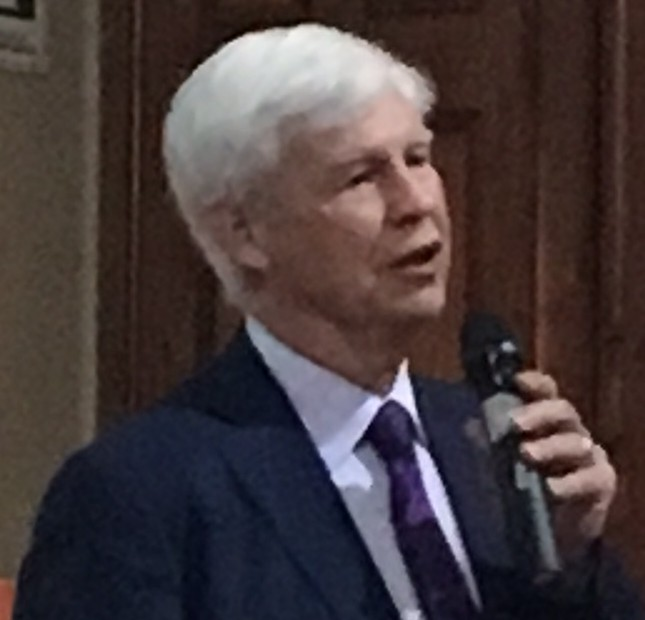
\includegraphics[height=0.3\textheight]{ch4_engle_2017.jpg}\\[1mm]
\imgcap{Robert F. Engle, 2017}
\imgcredit{https://commons.wikimedia.org/wiki/File:Robert_Engle_SantiagoWEAI2017.png}{Photo: Econterms (2017); CC BY-SA 4.0; Wikimedia Commons}
\end{column}
\begin{column}{0.68\textwidth}
\begin{itemize}
    \item DCC: a GARCH(1,1)-type recursion for a quasi-correlation matrix $Q_t$, rescaled into a correlation matrix
    \[ Q_t = (1 - a - b)S + a\,z_{t-1}z_{t-1}' + b\,Q_{t-1} \]
    \[ R_t = \mathrm{diag}(Q_t)^{-1/2}\,Q_t\,\mathrm{diag}(Q_t)^{-1/2} \]
    \begin{itemize}
        \item $z_t = D_t^{-1}\varepsilon_t$: standardised residuals of the univariate GARCH models; $S$: their sample correlation matrix (the target)
        \item $a \ge 0$: reaction of correlations to yesterday's co-movement; $b \ge 0$: persistence; $a + b < 1$
        \item $\mathrm{diag}(Q_t)$: the diagonal matrix of the diagonal elements of $Q_t$; the rescaling puts ones on the diagonal of $R_t$
    \end{itemize}
\end{itemize}
\end{column}
\end{columns}
\end{frame}

\begin{frame}{DCC and its corrected version cDCC (2/2): cDCC}
\itemsize{\small}
\begin{itemize}
    \item \refAie: the DCC target is estimated inconsistently
    \begin{itemize}
        \item $\E(z_tz_t' | \mathcal F_{t-1}) = R_t \ne Q_t$, so in general $\E Q_t \ne \E z_tz_t'$
        \item the moment estimator of $S$ is inconsistent, and so is $(\hat a, \hat b)$
    \end{itemize}
    \item cDCC: rescale the residuals by the diagonal of $Q_{t-1}$ before they enter the recursion
    \[ z^*_{t-1} = \mathrm{diag}(Q_{t-1})^{1/2}z_{t-1}, \qquad Q_t = (1 - a - b)S + a\,z^*_{t-1}z^{*\prime}_{t-1} + b\,Q_{t-1} \]
    \begin{itemize}
        \item then $\E(z^*_tz^{*\prime}_t | \mathcal F_{t-1}) = Q_t$, and $S = \E z^*_tz^{*\prime}_t$ is a valid target
        \item the cDCC target depends on $(a, b)$: it is estimated iteratively inside the likelihood
    \end{itemize}
\end{itemize}
\end{frame}

\begin{frame}{DCC against cDCC: a simulation}
\itemsize{\footnotesize}
\begin{center}
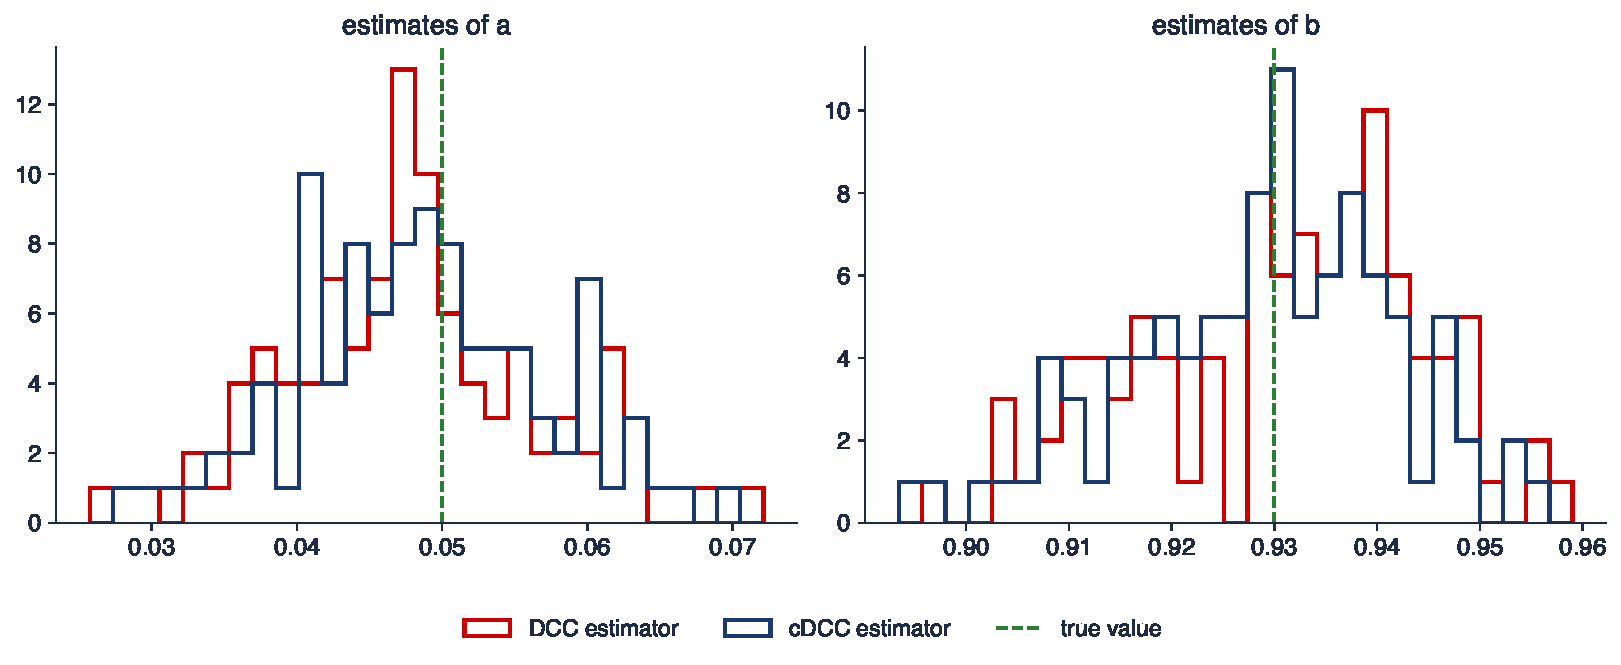
\includegraphics[width=0.97\textwidth,height=0.6\textheight,keepaspectratio]{ats_ch8_dcc_sim.pdf}
\end{center}
\vspace{-0.25cm}
\begin{itemize}
    \item Bivariate cDCC process with $a = 0.05$, $b = 0.93$, target correlation 0.5, unit variances; $T = 2\,000$, 100 replications; both estimators on each sample
\end{itemize}
\quantlet{ATS\_ch8\_mgarch}{\qlurl{ATS_ch8_mgarch}}
\end{frame}

\begin{frame}{Interpreting the DCC simulation}
\itemsize{\small}
\begin{itemize}
    \item Mean estimates: DCC $\hat a = 0.0478$, $\hat b = 0.9307$; cDCC $\hat a = 0.0486$, $\hat b = 0.9288$ (true 0.05 and 0.93)
    \item RMSE of $\hat a$: 0.0090 (DCC) and 0.0086 (cDCC); of $\hat b$: 0.0135 and 0.0129: the inconsistency is real but small at these persistence levels
    \item Sampling error dominates the bias with two thousand observations; the difference matters more for the target in large systems and for inference on $(a, b)$
    \item A proof of inconsistency does not tell you the size of the bias: simulate it in your own design before choosing an estimator
\end{itemize}
\end{frame}

\begin{frame}{Large covariance matrices: shrinkage and DCC-NL (1/2)}
\itemsize{\small}
\begin{itemize}
    \item With $N/T$ not small, the eigenvalues of a sample covariance $S$ are too dispersed
    \begin{itemize}
        \item $N$: number of assets; $T$: number of observations; the largest eigenvalues are too large, the smallest too small; the inverse $S^{-1}$ amplifies the error
    \end{itemize}
    \item Global minimum-variance (GMV) portfolio: the weights with the smallest variance that sum to 1
    \[ w = \frac{\Sigma^{-1}\mathbf 1}{\mathbf 1'\Sigma^{-1}\mathbf 1} \]
    \begin{itemize}
        \item $\Sigma$: covariance matrix of the returns; $\mathbf 1$: vector of ones
        \item it loads on the directions with the smallest, most underestimated eigenvalues
        \item it depends only on $\Sigma$, so its realised risk measures the quality of the covariance forecast without noise from expected returns
    \end{itemize}
\end{itemize}
\end{frame}

\begin{frame}{Large covariance matrices: shrinkage and DCC-NL (2/2)}
\itemsize{\small}
\begin{itemize}
    \item Linear shrinkage \refLWa: a weighted average of $S$ and a scaled identity
    \[ \hat\Sigma = \delta\,\mu I + (1 - \delta)\,S \]
    \begin{itemize}
        \item $\mu$: average eigenvalue of $S$; $\delta \in [0, 1]$: shrinkage intensity, estimated from the data (larger when $N/T$ is larger)
    \end{itemize}
    \item Nonlinear shrinkage \refLWb: keep the eigenvectors of $S$, replace each eigenvalue $\lambda_i$ by $d(\lambda_i)$
    \begin{itemize}
        \item $d(\cdot)$: an analytical kernel formula that pulls small eigenvalues up and large ones down, by different amounts
    \end{itemize}
    \item DCC-NL \refELW: in DCC, the target $S$ of the standardised residuals is itself a large sample covariance: replace it by its nonlinear shrinkage
    \begin{itemize}
        \item composite likelihood for $(a, b)$, univariate GARCH for the variances; evaluated by the out-of-sample s.d. of GMV portfolios
    \end{itemize}
\end{itemize}
\end{frame}

\begin{frame}{Case study: Engle, Ledoit and Wolf (2019) on US equities}
\itemsize{\footnotesize}
\begin{center}
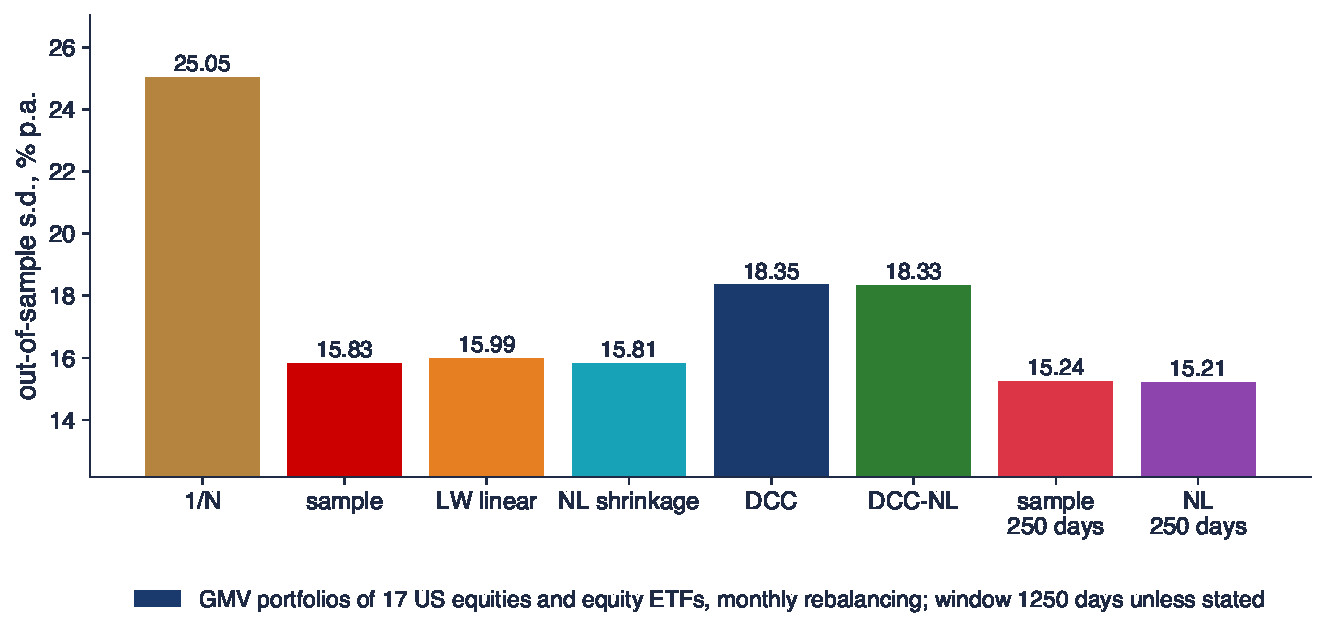
\includegraphics[width=0.97\textwidth,height=0.6\textheight,keepaspectratio]{ats_ch8_gmv.pdf}
\end{center}
\vspace{-0.25cm}
\begin{itemize}
    \item 17 assets: 14 US stocks and three equity ETFs (SPY, QQQ, RSP), which are portfolios of stocks; GMV weights rebalanced every 21 days from 23.05.2017 (112 rebalancings); window 1\,250 days, and 250 days for the last two bars; annualised out-of-sample s.d.
\end{itemize}
\quantlet{ATS\_ch8\_mgarch}{\qlurl{ATS_ch8_mgarch}}
\end{frame}

\begin{frame}{Interpreting the GMV comparison (1/2)}
\itemsize{\small}
\begin{itemize}
    \item Out-of-sample s.d. (\% p.a.): 1/N 25.05, sample 15.83, linear shrinkage 15.99, nonlinear shrinkage 15.81, DCC 18.35, DCC-NL 18.33
    \item With $N/T = 17/1\,250$ the sample covariance is already accurate
    \begin{itemize}
        \item nonlinear shrinkage changes little (15.81 against 15.83); DCC-NL is no better than DCC
    \end{itemize}
    \item Here the dynamics hurt: DCC gives 18.35 against 15.83
    \begin{itemize}
        \item DCC uses GARCH variances, with forecasts averaged over the 21-day holding period
        \item one-month-ahead variance forecasts of single stocks such as MSTR and TSLA are noisy, and GMV amplifies their errors
    \end{itemize}
\end{itemize}
\end{frame}

\begin{frame}{Interpreting the GMV comparison (2/2)}
\itemsize{\small}
\begin{itemize}
    \item A window of 250 days makes $N/T$ five times larger
    \begin{itemize}
        \item s.d. of the sample GMV 15.24, with nonlinear shrinkage 15.21: only 0.2\% lower
        \item yet the ETFs make the correlation matrix nearly singular (median condition number 1146)
        \item the shorter window itself lowers the risk: a crude form of time variation
    \end{itemize}
    \item The original study uses hundreds of stocks, where $N/T$ is large
    \begin{itemize}
        \item there the DCC-NL gains are substantial
        \item with our $N$ the lesson is when shrinkage matters, not how much it gains
    \end{itemize}
\end{itemize}
\end{frame}

\begin{frame}{Realised covariance}
\itemsize{\small}
\begin{itemize}
    \item The multivariate RV: the sum of outer products of the intraday return vectors
    \[ \mathrm{RCov}_t = \sum_{i=1}^n r_{t,i}\,r_{t,i}' \to \int_0^1\Sigma_s\,ds \]
    \begin{itemize}
        \item $r_{t,i}$: $N \times 1$ vector of intraday returns; $\Sigma_s$: spot covariance matrix; the limit adds the co-jumps (simultaneous jumps); with synchronous, noise-free prices it inherits the CLT of RV
    \end{itemize}
    \item Asynchronous trading: previous-tick prices create zero returns for the asset that has not traded; covariances shrink towards zero as the interval falls (the Epps effect)
    \begin{itemize}
        \item refresh-time sampling (all assets have traded) and the multivariate realised kernel \refBNHLSc: consistent and positive semi-definite
    \end{itemize}
    \item Forecasting: HAR on the elements of the Cholesky factor of $\mathrm{RCov}_t$ keeps forecasts positive definite \refCV; HEAVY and Realized GARCH have multivariate versions
    \item Evaluating covariance forecasts $H_t$ against a matrix proxy $\Sigma_t$: robust losses \refLRV
    \begin{itemize}
        \item matrix QLIKE $\ln|H_t| + \mathrm{tr}(H_t^{-1}\Sigma_t)$, with $|\cdot|$ the determinant and $\mathrm{tr}$ the trace; Frobenius MSE, the sum of squared element-wise errors
    \end{itemize}
\end{itemize}
\end{frame}

\begin{frame}{Bitcoin and Ether: realised and DCC correlation}
\itemsize{\footnotesize}
\begin{center}
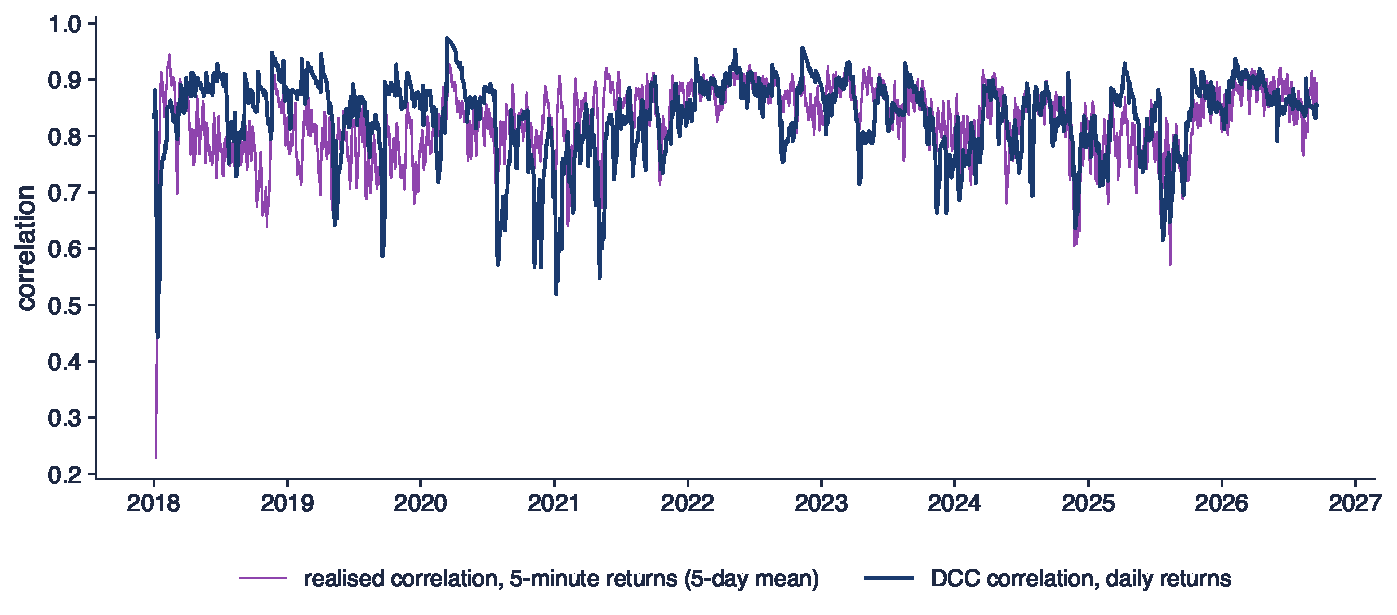
\includegraphics[width=0.97\textwidth,height=0.6\textheight,keepaspectratio]{ats_ch8_corr_crypto.pdf}
\end{center}
\vspace{-0.25cm}
\begin{itemize}
    \item Daily realised correlation from 5-minute returns (5-day means) and the DCC correlation of daily close-to-close (UTC) returns, 2018--2026
\end{itemize}
\quantlet{ATS\_ch8\_mgarch}{\qlurl{ATS_ch8_mgarch}}
\end{frame}

\begin{frame}{Interpreting the correlations}
\itemsize{\small}
\begin{itemize}
    \item Average realised correlation 0.83, average DCC correlation 0.83; correlation between the two series 0.26
    \item DCC uses one observation a day ($\hat a = 0.051$, $\hat b = 0.928$): it smooths and reacts with a lag; the realised measure moves daily and drops quickly in idiosyncratic episodes (5\% quantile 0.68)
    \item Combining both (a realised measure in the correlation equation) is the multivariate analogue of Realized GARCH
    \item Five-minute sampling sits on the flat part of the Epps curve for these two coins (signature slide): the realised correlation is not biased towards zero
\end{itemize}
\end{frame}

\begin{frame}{Recap: Multivariate}
\itemsize{\small}
\begin{itemize}
    \item BEKK guarantees positivity at a quadratic parameter cost; DCC separates variances and correlations and scales to large $N$
    \item cDCC fixes the inconsistency of the DCC target; in moderate designs the difference is small
    \item In high dimension, the target needs shrinkage (DCC-NL); evaluate with GMV risk or robust matrix losses
\end{itemize}
\end{frame}


%=============================================================================
\section{AI for scientific discovery}
%=============================================================================

\begin{frame}{An open question}
\itemsize{\small}
\begin{itemize}
    \item Does exploiting the measurement error of realised variance (HARQ) improve volatility forecasts robustly, or only under particular design choices?
    \begin{itemize}
        \item formal: the QLIKE ratio HARQ/HAR and its DM statistic across a pre-registered grid (window, filter, realised measure, asset); falsified if the ratio exceeds 1 or the DM test is insignificant for most cells
        \item the measure of precision (RQ) is itself noisy and fat-tailed, so the gain may be fragile
    \end{itemize}
    \item Why it matters: risk systems use one-day volatility forecasts every day; a small but robust gain is worth more than a large fragile one
    \begin{itemize}
        \item literature to start from: \refBPQ, \refCor, \refPat, \refHLb, \refHLN
    \end{itemize}
\end{itemize}
\end{frame}

\begin{frame}{The discovery loop with an AI assistant}
\itemsize{\footnotesize}
\begin{itemize}
    \item An AI assistant (an LLM such as Claude, ChatGPT, Gemini or Copilot) speeds up each step; Semantic Scholar and Elicit help with the literature
    \begin{itemize}
        \item \textbf{literature}: \aiprompt{List peer-reviewed papers since 2016 that test HARQ-type models out of sample on assets other than US equities; give DOIs.} Then check every DOI on Crossref
        \item \textbf{hypothesis}: \aiprompt{Under which data features (24/7 trading, jumps, zero returns) should the HARQ gain shrink or grow? Give testable predictions.}
        \item \textbf{code and replication}: ask for HAR and HARQ rolling forecasts, then reproduce a known number first (the Bitcoin QLIKE ratio of this lecture)
        \item \textbf{robustness and critique}: \aiprompt{Act as a hostile referee: which choices in a HARQ forecast comparison could produce a spurious gain?}
    \end{itemize}
    \item Report: what was asked, what was kept, what was rejected (AI\_USE.md, AI\_ERRORS.md)
\end{itemize}
\end{frame}

\begin{frame}{What the human checks}
\itemsize{\small}
\begin{itemize}
    \item Every reference exists and says what is claimed (DOI resolves, title matches, the result is in the paper)
    \item The forecast at $t$ uses only data up to $t$: windows, demeaning of RQ, the insanity filter and the bias correction of log forecasts are all computed in the estimation window
    \item The loss is robust (QLIKE, MSE) and the proxy is stated; DM statistics use HAC variances
    \item All cells of the grid are reported, not the best one; the number of comparisons is stated
    \item Realised measures are recomputed from raw prices and agree with an independent source on overlapping assets and dates
\end{itemize}
\end{frame}

\begin{frame}{Mini-case: twelve choices, one conclusion?}
\itemsize{\footnotesize}
\begin{center}
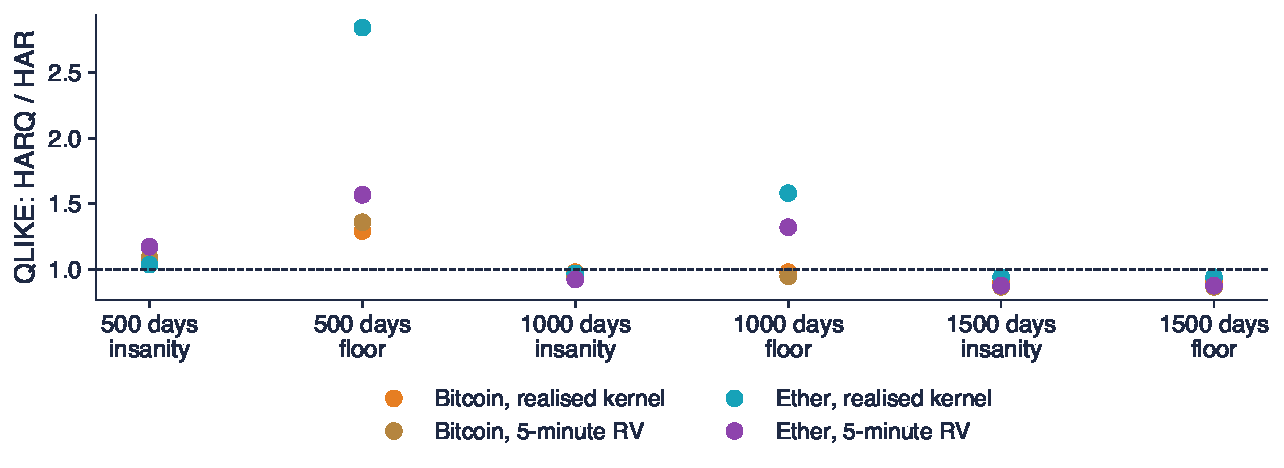
\includegraphics[width=0.97\textwidth,height=0.6\textheight,keepaspectratio]{ats_ch8_ai_case.pdf}
\end{center}
\vspace{-0.25cm}
\begin{itemize}
    \item QLIKE ratio HARQ/HAR for Bitcoin and Ether: window 500, 1\,000 or 1\,500 days; insanity filter or a floor at the smallest in-sample RV; target 5-minute RV or realised kernel
    \item Ratios from 0.865 to 2.844; HARQ better in 58\% of the 24 cells, significantly better (DM $< -1.96$) in 50\%, significantly worse in 12\%: an AI summary reporting one cell would hide most of this
\end{itemize}
\quantlet{ATS\_ch8\_ai\_robustness}{\qlurl{ATS_ch8_ai_robustness}}
\end{frame}

\begin{frame}{Project idea}
\itemsize{\small}
\begin{itemize}
    \item \textbf{Realised volatility of crypto-assets: does the equity toolkit transfer?}: replicate first, then extend
    \begin{itemize}
        \item replicate: HAR and HARQ of this lecture for Bitcoin (QLIKE ratio 0.946) and Realized GARCH for the S\&P 500 (persistence 0.968)
        \item extend: ten coins from the Binance archive; noise-robust measures from one-second data
        \item extend the tests: an intraday seasonality correction before jump tests; Realized GARCH with the realised kernel
        \item use the spot-ETF date (January 2024) as a natural break
        \item pre-register: assets, sample, measures, models, windows, losses, the DM/MCS tests and the robustness grid
    \end{itemize}
    \item Deliverables follow the course rules: repository, report, AI\_USE.md, AI\_ERRORS.md, oral defence
\end{itemize}
\end{frame}


%=============================================================================
\section{Wrap-up}
%=============================================================================

\begin{frame}{Key takeaways}
\itemsize{\small}
\begin{itemize}
    \item Gaussian QML needs only the variance equation; with fat tails, use sandwich standard errors
    \item Volatility has fast and slow components; macro drivers of the slow one need long samples and honest variance ratios
    \item Realised measures make volatility observable with a known error; noise and jumps decide the estimator
    \item HAR, HARQ and Realized GARCH beat return-only models one day ahead; evaluate with QLIKE or MSE
    \item In many dimensions the correlation target needs shrinkage (DCC-NL); whether the dynamics help must be checked out of sample
\end{itemize}
\end{frame}

\begin{frame}{Self-assessment}
\itemsize{\small}
\begin{columns}[T]
\begin{column}{0.58\textwidth}
\begin{block}{Questions}
\begin{itemize}
    \item Why are Hessian standard errors too small for GARCH when $\kappa_\eta > 3$?
    \item What does the variance ratio of GARCH-MIDAS measure?
    \item Why does stable convergence matter for the CLT of RV?
    \item Why can a signature plot rise at high frequency?
    \item Why is $\beta_{dQ}$ expected to be negative in HARQ?
    \item Which losses keep the ranking under a noisy proxy?
\end{itemize}
\end{block}
\end{column}
\begin{column}{0.38\textwidth}
\begin{block}{Next: \atschlink{https://danpele.github.io/Advanced-Time-Series/EN/Courses/chapter9_var_es_backtesting.pdf}{Chapter 9}}
\begin{itemize}
    \item VaR, ES and backtesting: elicitability, scoring and model risk
    \item From volatility forecasts to tail forecasts: VaR 1\% and ES 2.5\%, their scoring functions and backtests
\end{itemize}
\end{block}
\end{column}
\end{columns}
\end{frame}


%=============================================================================
\section{Appendix}
%=============================================================================

\begin{frame}{Appendix: the GARCH sandwich}
\hypertarget{atsapp1}{}\atsappback{atssrc1}{Back}
\itemsize{\small}
\begin{itemize}
    \item $\ell_t = -\frac12(\ln\sigma^2_t + \varepsilon^2_t/\sigma^2_t)$, $d_t = \sigma_t^{-2}\partial\sigma^2_t/\partial\theta$: $s_t = \frac12(\eta^2_t - 1)d_t$ at $\theta_0$
    \item $B = \E s_ts_t' = \frac14\E(\eta^2_t - 1)^2\,\E d_td_t' = \frac{\kappa_\eta - 1}{4}J$, because $\eta_t$ is independent of $d_t \in \mathcal F_{t-1}$
    \item $\partial s_t/\partial\theta' = -\frac12\eta^2_td_td_t' + \frac12(\eta^2_t - 1)\partial d_t/\partial\theta'$; the second term has mean zero, so $A = \frac12J$
    \item $A^{-1}B\,A^{-1} = 4J^{-1}\cdot\frac{\kappa_\eta - 1}{4}J\cdot J^{-1} = (\kappa_\eta - 1)J^{-1}$; Hessian only: $A^{-1} = 2J^{-1}$; OPG: $B^{-1} = \frac{4}{\kappa_\eta - 1}J^{-1}$
\end{itemize}
\end{frame}

\begin{frame}{Appendix: the noise bias of realised variance}
\hypertarget{atsapp2}{}\atsappback{atssrc2}{Back}
\itemsize{\small}
\begin{itemize}
    \item $\tilde r_i = Y_{i/n} - Y_{(i-1)/n} = r_i + u_i - u_{i-1}$, with $u$ i.i.d. $(0, \omega^2)$ independent of $X$
    \item $\sum_i\tilde r_i^2 = \sum_ir_i^2 + 2\sum_ir_i(u_i - u_{i-1}) + \sum_i(u_i - u_{i-1})^2$; the cross term has mean zero, the last has mean $2n\omega^2$
    \item $\Cov(\tilde r_i, \tilde r_{i-1}) = -\omega^2$: first-order negative autocorrelation; the realised kernel adds $2\gamma_1 \approx -2n\omega^2$ back and removes the bias
    \item Positively autocorrelated returns (gradual price adjustment, stale prices) give $\gamma_1 > 0$ and a signature plot that rises with the interval; the kernel corrects both signs
\end{itemize}
\end{frame}

\begin{frame}{Appendix: attenuation and HARQ}
\hypertarget{atsapp3}{}\atsappback{atssrc3}{Back}
\itemsize{\small}
\begin{itemize}
    \item $\mathrm{IV}_{t+1} = c + \phi\,\mathrm{IV}_t + v_{t+1}$, observed $\mathrm{RV}_t = \mathrm{IV}_t + e_t$, $e_t$ uncorrelated with $\mathrm{IV}_t$ and $v_{t+1}$
    \item OLS of $\mathrm{RV}_{t+1}$ on $\mathrm{RV}_t$: $\mathrm{plim}\,\hat\phi = \frac{\Cov(\mathrm{IV}_{t+1}, \mathrm{IV}_t)}{\Var(\mathrm{IV}_t) + \Var(e_t)} = \phi\lambda$, $\lambda = \frac{\Var(\mathrm{IV})}{\Var(\mathrm{IV}) + \E\Var(e_t)}$
    \item The best linear predictor given today's precision uses $\phi\lambda_t$, $\lambda_t = \frac{\Var(\mathrm{IV})}{\Var(\mathrm{IV}) + 2\mathrm{IQ}_t/n}$: decreasing in $\mathrm{IQ}_t$
    \item A first-order expansion in $\sqrt{\mathrm{IQ}_t}$ gives $\beta_d + \beta_{dQ}\sqrt{\mathrm{RQ}_t}$ with $\beta_{dQ} < 0$: the HARQ specification \refBPQ
\end{itemize}
\end{frame}


%=============================================================================
\section{References}
%=============================================================================

\begin{frame}{References (1/5)}
\itemsize{\tiny}
\begin{itemize}
    \item Aielli, G. P. (2013). Dynamic conditional correlation: On properties and estimation. \textit{Journal of Business \& Economic Statistics}, 31(3), 282--299. \href{https://doi.org/10.1080/07350015.2013.771027}{doi:10.1080/07350015.2013.771027}
    \item Andersen, T. G., \& Bollerslev, T. (1998). Answering the skeptics: Yes, standard volatility models do provide accurate forecasts. \textit{International Economic Review}, 39(4), 885--905. \href{https://doi.org/10.2307/2527343}{doi:10.2307/2527343}
    \item Andersen, T. G., Bollerslev, T., \& Diebold, F. X. (2007). Roughing it up: Including jump components in the measurement, modeling, and forecasting of return volatility. \textit{The Review of Economics and Statistics}, 89(4), 701--720. \href{https://doi.org/10.1162/rest.89.4.701}{doi:10.1162/rest.89.4.701}
    \item Andersen, T. G., Bollerslev, T., Diebold, F. X., \& Labys, P. (2003). Modeling and forecasting realized volatility. \textit{Econometrica}, 71(2), 579--625. \href{https://doi.org/10.1111/1468-0262.00418}{doi:10.1111/1468-0262.00418}
    \item Andersen, T. G., Dobrev, D., \& Schaumburg, E. (2012). Jump-robust volatility estimation using nearest neighbor truncation. \textit{Journal of Econometrics}, 169(1), 75--93. \href{https://doi.org/10.1016/j.jeconom.2012.01.011}{doi:10.1016/j.jeconom.2012.01.011}
    \item Bandi, F. M., \& Russell, J. R. (2008). Microstructure noise, realized variance, and optimal sampling. \textit{The Review of Economic Studies}, 75(2), 339--369. \href{https://doi.org/10.1111/j.1467-937X.2008.00474.x}{doi:10.1111/j.1467-937X.2008.00474.x}
    \item Barndorff-Nielsen, O. E., Hansen, P. R., Lunde, A., \& Shephard, N. (2008). Designing realized kernels to measure the ex post variation of equity prices in the presence of noise. \textit{Econometrica}, 76(6), 1481--1536. \href{https://doi.org/10.3982/ECTA6495}{doi:10.3982/ECTA6495}
    \item Barndorff-Nielsen, O. E., Hansen, P. R., Lunde, A., \& Shephard, N. (2009). Realized kernels in practice: Trades and quotes. \textit{The Econometrics Journal}, 12(3), C1--C32. \href{https://doi.org/10.1111/j.1368-423X.2008.00275.x}{doi:10.1111/j.1368-423X.2008.00275.x}
    \item Barndorff-Nielsen, O. E., Hansen, P. R., Lunde, A., \& Shephard, N. (2011). Multivariate realised kernels: Consistent positive semi-definite estimators of the covariation of equity prices with noise and non-synchronous trading. \textit{Journal of Econometrics}, 162(2), 149--169. \href{https://doi.org/10.1016/j.jeconom.2010.07.009}{doi:10.1016/j.jeconom.2010.07.009}
    \item Barndorff-Nielsen, O. E., \& Shephard, N. (2002). Econometric analysis of realized volatility and its use in estimating stochastic volatility models. \textit{Journal of the Royal Statistical Society: Series B}, 64(2), 253--280. \href{https://doi.org/10.1111/1467-9868.00336}{doi:10.1111/1467-9868.00336}
    \item Barndorff-Nielsen, O. E., \& Shephard, N. (2004). Power and bipower variation with stochastic volatility and jumps. \textit{Journal of Financial Econometrics}, 2(1), 1--37. \href{https://doi.org/10.1093/jjfinec/nbh001}{doi:10.1093/jjfinec/nbh001}
    \item Barndorff-Nielsen, O. E., \& Shephard, N. (2006). Econometrics of testing for jumps in financial economics using bipower variation. \textit{Journal of Financial Econometrics}, 4(1), 1--30. \href{https://doi.org/10.1093/jjfinec/nbi022}{doi:10.1093/jjfinec/nbi022}
\end{itemize}
\end{frame}

\begin{frame}{References (2/5)}
\itemsize{\tiny}
\begin{itemize}
    \item Berkes, I., Horváth, L., \& Kokoszka, P. (2003). GARCH processes: Structure and estimation. \textit{Bernoulli}, 9(2), 201--227. \href{https://doi.org/10.3150/bj/1068128975}{doi:10.3150/bj/1068128975}
    \item Bollerslev, T. (1986). Generalized autoregressive conditional heteroskedasticity. \textit{Journal of Econometrics}, 31(3), 307--327. \href{https://doi.org/10.1016/0304-4076(86)90063-1}{doi:10.1016/0304-4076(86)90063-1}
    \item Bollerslev, T. (1990). Modelling the coherence in short-run nominal exchange rates: A multivariate generalized ARCH model. \textit{The Review of Economics and Statistics}, 72(3), 498--505. \href{https://doi.org/10.2307/2109358}{doi:10.2307/2109358}
    \item Bollerslev, T., Patton, A. J., \& Quaedvlieg, R. (2016). Exploiting the errors: A simple approach for improved volatility forecasting. \textit{Journal of Econometrics}, 192(1), 1--18. \href{https://doi.org/10.1016/j.jeconom.2015.10.007}{doi:10.1016/j.jeconom.2015.10.007}
    \item Bollerslev, T., \& Wooldridge, J. M. (1992). Quasi-maximum likelihood estimation and inference in dynamic models with time-varying covariances. \textit{Econometric Reviews}, 11(2), 143--172. \href{https://doi.org/10.1080/07474939208800229}{doi:10.1080/07474939208800229}
    \item Chiriac, R., \& Voev, V. (2011). Modelling and forecasting multivariate realized volatility. \textit{Journal of Applied Econometrics}, 26(6), 922--947. \href{https://doi.org/10.1002/jae.1152}{doi:10.1002/jae.1152}
    \item Comte, F., \& Lieberman, O. (2003). Asymptotic theory for multivariate GARCH processes. \textit{Journal of Multivariate Analysis}, 84(1), 61--84. \href{https://doi.org/10.1016/S0047-259X(02)00009-X}{doi:10.1016/S0047-259X(02)00009-X}
    \item Conrad, C., \& Kleen, O. (2020). Two are better than one: Volatility forecasting using multiplicative component GARCH-MIDAS models. \textit{Journal of Applied Econometrics}, 35(1), 19--45. \href{https://doi.org/10.1002/jae.2742}{doi:10.1002/jae.2742}
    \item Corsi, F. (2009). A simple approximate long-memory model of realized volatility. \textit{Journal of Financial Econometrics}, 7(2), 174--196. \href{https://doi.org/10.1093/jjfinec/nbp001}{doi:10.1093/jjfinec/nbp001}
    \item Diebold, F. X., \& Mariano, R. S. (1995). Comparing predictive accuracy. \textit{Journal of Business \& Economic Statistics}, 13(3), 253--263. \href{https://doi.org/10.1080/07350015.1995.10524599}{doi:10.1080/07350015.1995.10524599}
    \item Engle, R. (2002). Dynamic conditional correlation: A simple class of multivariate generalized autoregressive conditional heteroskedasticity models. \textit{Journal of Business \& Economic Statistics}, 20(3), 339--350. \href{https://doi.org/10.1198/073500102288618487}{doi:10.1198/073500102288618487}
    \item Engle, R. F. (1982). Autoregressive conditional heteroscedasticity with estimates of the variance of United Kingdom inflation. \textit{Econometrica}, 50(4), 987--1007. \href{https://doi.org/10.2307/1912773}{doi:10.2307/1912773}
\end{itemize}
\end{frame}

\begin{frame}{References (3/5)}
\itemsize{\tiny}
\begin{itemize}
    \item Engle, R. F., Ghysels, E., \& Sohn, B. (2013). Stock market volatility and macroeconomic fundamentals. \textit{The Review of Economics and Statistics}, 95(3), 776--797. \href{https://doi.org/10.1162/REST_a_00300}{doi:10.1162/REST\_a\_00300}
    \item Engle, R. F., \& Kroner, K. F. (1995). Multivariate simultaneous generalized ARCH. \textit{Econometric Theory}, 11(1), 122--150. \href{https://doi.org/10.1017/S0266466600009063}{doi:10.1017/S0266466600009063}
    \item Engle, R. F., Ledoit, O., \& Wolf, M. (2019). Large dynamic covariance matrices. \textit{Journal of Business \& Economic Statistics}, 37(2), 363--375. \href{https://doi.org/10.1080/07350015.2017.1345683}{doi:10.1080/07350015.2017.1345683}
    \item Engle, R. F., \& Lee, G. G. J. (1999). A long-run and short-run component model of stock return volatility. In R. F. Engle \& H. White (Eds.), \textit{Cointegration, Causality, and Forecasting: A Festschrift in Honour of Clive W. J. Granger} (pp.\ 475--497). Oxford University Press. \href{https://doi.org/10.1093/oso/9780198296836.003.0020}{doi:10.1093/oso/9780198296836.003.0020}
    \item Engle, R. F., \& Sheppard, K. (2001). Theoretical and empirical properties of dynamic conditional correlation multivariate GARCH. \textit{NBER Working Paper} 8554. \href{https://doi.org/10.3386/w8554}{doi:10.3386/w8554}
    \item Epps, T. W. (1979). Comovements in stock prices in the very short run. \textit{Journal of the American Statistical Association}, 74(366), 291--298. \href{https://doi.org/10.1080/01621459.1979.10482508}{doi:10.1080/01621459.1979.10482508}
    \item Francq, C., \& Zakoïan, J.-M. (2004). Maximum likelihood estimation of pure GARCH and ARMA-GARCH processes. \textit{Bernoulli}, 10(4), 605--637. \href{https://doi.org/10.3150/bj/1093265632}{doi:10.3150/bj/1093265632}
    \item Francq, C., \& Zakoïan, J.-M. (2019). \textit{GARCH Models: Structure, Statistical Inference and Financial Applications} (2nd ed.). Wiley. \href{https://doi.org/10.1002/9781119313472}{doi:10.1002/9781119313472}
    \item Ghysels, E., Santa-Clara, P., \& Valkanov, R. (2006). Predicting volatility: Getting the most out of return data sampled at different frequencies. \textit{Journal of Econometrics}, 131(1--2), 59--95. \href{https://doi.org/10.1016/j.jeconom.2005.01.004}{doi:10.1016/j.jeconom.2005.01.004}
    \item Glosten, L. R., Jagannathan, R., \& Runkle, D. E. (1993). On the relation between the expected value and the volatility of the nominal excess return on stocks. \textit{The Journal of Finance}, 48(5), 1779--1801. \href{https://doi.org/10.1111/j.1540-6261.1993.tb05128.x}{doi:10.1111/j.1540-6261.1993.tb05128.x}
    \item Hafner, C. M., \& Preminger, A. (2009). On asymptotic theory for multivariate GARCH models. \textit{Journal of Multivariate Analysis}, 100(9), 2044--2054. \href{https://doi.org/10.1016/j.jmva.2009.03.011}{doi:10.1016/j.jmva.2009.03.011}
    \item Hamilton, J. D. (1994). \textit{Time Series Analysis}. Princeton University Press. \href{https://doi.org/10.2307/j.ctv14jx6sm}{doi:10.2307/j.ctv14jx6sm}
\end{itemize}
\end{frame}

\begin{frame}{References (4/5)}
\itemsize{\tiny}
\begin{itemize}
    \item Hansen, P. R., \& Huang, Z. (2016). Exponential GARCH modeling with realized measures of volatility. \textit{Journal of Business \& Economic Statistics}, 34(2), 269--287. \href{https://doi.org/10.1080/07350015.2015.1038543}{doi:10.1080/07350015.2015.1038543}
    \item Hansen, P. R., Huang, Z., \& Shek, H. H. (2012). Realized GARCH: A joint model for returns and realized measures of volatility. \textit{Journal of Applied Econometrics}, 27(6), 877--906. \href{https://doi.org/10.1002/jae.1234}{doi:10.1002/jae.1234}
    \item Hansen, P. R., \& Lunde, A. (2005). A forecast comparison of volatility models: Does anything beat a GARCH(1,1)? \textit{Journal of Applied Econometrics}, 20(7), 873--889. \href{https://doi.org/10.1002/jae.800}{doi:10.1002/jae.800}
    \item Hansen, P. R., \& Lunde, A. (2006a). Consistent ranking of volatility models. \textit{Journal of Econometrics}, 131(1--2), 97--121. \href{https://doi.org/10.1016/j.jeconom.2005.01.005}{doi:10.1016/j.jeconom.2005.01.005}
    \item Hansen, P. R., \& Lunde, A. (2006b). Realized variance and market microstructure noise. \textit{Journal of Business \& Economic Statistics}, 24(2), 127--161. \href{https://doi.org/10.1198/073500106000000071}{doi:10.1198/073500106000000071}
    \item Hansen, P. R., Lunde, A., \& Nason, J. M. (2011). The model confidence set. \textit{Econometrica}, 79(2), 453--497. \href{https://doi.org/10.3982/ECTA5771}{doi:10.3982/ECTA5771}
    \item Heber, G., Lunde, A., Shephard, N., \& Sheppard, K. (2009). \textit{Oxford-Man Institute's realized library}, version 0.3. Oxford-Man Institute, University of Oxford (discontinued in 2022; copy of 28 February 2022 preserved by the Internet Archive). \href{https://web.archive.org/web/2021/https://realized.oxford-man.ox.ac.uk/terms-and-conditions}{web.archive.org}
    \item Huang, X., \& Tauchen, G. (2005). The relative contribution of jumps to total price variance. \textit{Journal of Financial Econometrics}, 3(4), 456--499. \href{https://doi.org/10.1093/jjfinec/nbi025}{doi:10.1093/jjfinec/nbi025}
    \item Jacod, J., Li, Y., Mykland, P. A., Podolskij, M., \& Vetter, M. (2009). Microstructure noise in the continuous case: The pre-averaging approach. \textit{Stochastic Processes and their Applications}, 119(7), 2249--2276. \href{https://doi.org/10.1016/j.spa.2008.11.004}{doi:10.1016/j.spa.2008.11.004}
    \item Jensen, S. T., \& Rahbek, A. (2004). Asymptotic inference for nonstationary GARCH. \textit{Econometric Theory}, 20(6), 1203--1226. \href{https://doi.org/10.1017/S0266466604206065}{doi:10.1017/S0266466604206065}
    \item Laurent, S., Rombouts, J. V. K., \& Violante, F. (2012). On the forecasting accuracy of multivariate GARCH models. \textit{Journal of Applied Econometrics}, 27(6), 934--955. \href{https://doi.org/10.1002/jae.1248}{doi:10.1002/jae.1248}
    \item Ledoit, O., \& Wolf, M. (2004). A well-conditioned estimator for large-dimensional covariance matrices. \textit{Journal of Multivariate Analysis}, 88(2), 365--411. \href{https://doi.org/10.1016/S0047-259X(03)00096-4}{doi:10.1016/S0047-259X(03)00096-4}
\end{itemize}
\end{frame}

\begin{frame}{References (5/5)}
\itemsize{\tiny}
\begin{itemize}
    \item Ledoit, O., \& Wolf, M. (2020). Analytical nonlinear shrinkage of large-dimensional covariance matrices. \textit{The Annals of Statistics}, 48(5), 3043--3065. \href{https://doi.org/10.1214/19-AOS1921}{doi:10.1214/19-AOS1921}
    \item Lee, S. S., \& Mykland, P. A. (2008). Jumps in financial markets: A new nonparametric test and jump dynamics. \textit{The Review of Financial Studies}, 21(6), 2535--2563. \href{https://doi.org/10.1093/rfs/hhm056}{doi:10.1093/rfs/hhm056}
    \item Lee, S.-W., \& Hansen, B. E. (1994). Asymptotic theory for the GARCH(1,1) quasi-maximum likelihood estimator. \textit{Econometric Theory}, 10(1), 29--52. \href{https://doi.org/10.1017/S0266466600008215}{doi:10.1017/S0266466600008215}
    \item Ling, S., \& McAleer, M. (2003). Asymptotic theory for a vector ARMA-GARCH model. \textit{Econometric Theory}, 19(2), 280--310. \href{https://doi.org/10.1017/S0266466603192092}{doi:10.1017/S0266466603192092}
    \item Lumsdaine, R. L. (1996). Consistency and asymptotic normality of the quasi-maximum likelihood estimator in IGARCH(1,1) and covariance stationary GARCH(1,1) models. \textit{Econometrica}, 64(3), 575--596. \href{https://doi.org/10.2307/2171862}{doi:10.2307/2171862}
    \item Newey, W. K., \& West, K. D. (1987). A simple, positive semi-definite, heteroskedasticity and autocorrelation consistent covariance matrix. \textit{Econometrica}, 55(3), 703--708. \href{https://doi.org/10.2307/1913610}{doi:10.2307/1913610}
    \item Pakel, C., Shephard, N., Sheppard, K., \& Engle, R. F. (2021). Fitting vast dimensional time-varying covariance models. \textit{Journal of Business \& Economic Statistics}, 39(3), 652--668. \href{https://doi.org/10.1080/07350015.2020.1713795}{doi:10.1080/07350015.2020.1713795}
    \item Patton, A. J. (2011). Volatility forecast comparison using imperfect volatility proxies. \textit{Journal of Econometrics}, 160(1), 246--256. \href{https://doi.org/10.1016/j.jeconom.2010.03.034}{doi:10.1016/j.jeconom.2010.03.034}
    \item Patton, A. J., \& Sheppard, K. (2015). Good volatility, bad volatility: Signed jumps and the persistence of volatility. \textit{The Review of Economics and Statistics}, 97(3), 683--697. \href{https://doi.org/10.1162/REST_a_00503}{doi:10.1162/REST\_a\_00503}
    \item Petropoulos, F., Apiletti, D., Assimakopoulos, V., Babai, M. Z., et al.\ (2022). Forecasting: Theory and practice. \textit{International Journal of Forecasting}, 38(3), 705--871. \href{https://doi.org/10.1016/j.ijforecast.2021.11.001}{doi:10.1016/j.ijforecast.2021.11.001}
    \item Shephard, N., \& Sheppard, K. (2010). Realising the future: Forecasting with high-frequency-based volatility (HEAVY) models. \textit{Journal of Applied Econometrics}, 25(2), 197--231. \href{https://doi.org/10.1002/jae.1158}{doi:10.1002/jae.1158}
    \item Zhang, L., Mykland, P. A., \& Aït-Sahalia, Y. (2005). A tale of two time scales: Determining integrated volatility with noisy high-frequency data. \textit{Journal of the American Statistical Association}, 100(472), 1394--1411. \href{https://doi.org/10.1198/016214505000000169}{doi:10.1198/016214505000000169}
\end{itemize}
\end{frame}

\end{document}
